\documentclass[12pt,a4paper]{report}
\usepackage{fullpage}
\usepackage[utf8x]{vietnam}
\usepackage[fontsize=13pt]{scrextend}
\usepackage{graphicx}%Thư viện chèn ảnh
\usepackage[unicode]{hyperref}
\usepackage{tikz}
\usepackage{newtxmath}%Time New Roman
\usepackage{float} %Set vị trí chèn ảnh
\usepackage{array}
\usepackage{indentfirst} %Thư viện thụt đầu dòng
\usepackage{multirow}
\usepackage{longtable}
\usepackage{tocloft}
\usepackage{enumerate}

\renewcommand{\baselinestretch}{1.2} %Giãn dòng 1.2
\setlength{\parskip}{6pt} %Spacing after
\setlength{\parindent}{1cm} %Set khoảng cách thụt đầu dòng mỗi đoạn
\usepackage{titlesec}%Thư viện set up các kiểu chữ
\setcounter{secnumdepth}{4}

\usepackage{calc}

\usepackage{lipsum} 

\renewcommand{\contentsname}{MỤC LỤC}
\renewcommand{\listfigurename}{DANH MỤC HÌNH VẼ}
\renewcommand{\listtablename}{DANH MỤC BẢNG BIỂU}

\titlespacing*{\section}{0pt}{0pt}{15pt} %Heading 1
\titleformat*{\section}{\fontsize{16pt}{0pt}\selectfont \bfseries \centering}

\titlespacing*{\subsection}{0pt}{10pt}{0pt} %Heading 2
\titleformat*{\subsection}{\fontsize{14pt}{0pt}\selectfont \bfseries}

\titlespacing*{\subsubsection}{0pt}{10pt}{0pt} %Heading 3
\titleformat*{\subsubsection}{\fontsize{13pt}{0pt}\selectfont \bfseries \itshape}

\titlespacing*{\paragraph}{0pt}{10pt}{0pt} %Heading 4
\titleformat*{\paragraph}{\fontsize{13pt}{0pt}\selectfont \bfseries}

\renewcommand{\figurename}{\fontsize{12pt}{0pt}\selectfont Hình}
\renewcommand{\thefigure}{\thesection.\arabic{figure}}
\usepackage{caption}
\captionsetup[figure]{labelsep=space}

\renewcommand{\tablename}{\fontsize{12pt}{0pt}\selectfont Bảng}
\renewcommand{\thetable}{\thesection.\arabic{table}}
\captionsetup[table]{labelsep=space}

\usepackage{tabularx}
\newcolumntype{s}{>{\hsize=.4\hsize}X}
\newcolumntype{a}{>{\hsize=1.2\hsize}X}
\usepackage{indentfirst}
\setlength{\parindent}{20pt}
\hypersetup{
    colorlinks=true,
    linkcolor=black,
    filecolor=magenta,      
    urlcolor=cyan,
}

\title{\textbf{BÁO CÁO CUỐI KỲ}\\
\textbf{GIAO THỨC VÀ MẠNG MÁY TÍNH}\\
\vspace{15pt}
\textbf{
THIẾT KẾ HỆ THỐNG MẠNG DOANH NGHIỆP CÓ HAI CHI NHÁNH}\\
}
\author{}
\date{}

\begin{document}


\begin{center} 
\large TỔNG LIÊN ĐOÀN LAO ĐỘNG VIỆT NAM
\\ \textbf{TRƯỜNG ĐẠI HỌC TÔN ĐỨC THẮNG} 
\\ \textbf{KHOA CÔNG NGHỆ THÔNG TIN} 
\large
\end{center}

\begin{center}
\includegraphics[width=4cm]{img/TDT\_logo.png}
\end{center}
\vfill

\begingroup
\let\newpage\relax
\maketitle
\thispagestyle{empty}
\endgroup

\begin{flushright}
\textit{Người hướng dẫn}:
\textbf{TS. TRƯƠNG ĐÌNH TÚ }\\
\vspace{5pt}
\textit{Người thực hiện}:
\textbf{NGÔ HỮU LỄ – 51800571}\\
\vspace{5pt}
\textbf{PHẠM NHẬT ANH  – 51900646}\\
\vspace{5pt}
\textit{Khóa}:
\textbf{22, 23}\\
\vspace{5pt}
\begin{center} 
\large \textbf{THÀNH PHỐ HỒ CHÍ MINH, NĂM 2023}
\large
\end{center}
\end{flushright}
\vfill
\cleardoublepage


\section*{LỜI CẢM ƠN}
\phantomsection
\thispagestyle{empty}
\hspace*{0.25cm}Đầu tiên, nhóm em xin gửi lời cảm ơn đến Khoa Công nghệ thông tin trường đại học Tôn Đức Thắng đã tạo điều kiện cho chúng em được tham gia học tập môn học này. Ngoài ra khoa còn tạo điều kiện để chúng em có cơ hội hoàn thành môn học một cách tốt nhất.\\
\hspace*{1cm}Tiếp theo, nhóm em xin gửi lời cảm ơn đến thầy Trương Đình Tú đã hướng dẫn, chỉ dạy chúng em trong suốt quá trình học và hoàn thành bài báo cáo này. Và bên cạnh đó, chúng em cũng xin cảm ơn đến thầy cô giảng viên tại trường, đặt biệt là  các giảng viên trong trong khoa Công Nghệ Thông Tin đã dạy chúng em nhiều kiến thức cơ bản, thiết yếu và trang bị cho chúng em một lượng tri thức trong suốt quá trình học cũng như trong quá trình làm bài báo cáo.\\
\hspace*{1cm}Cuối cùng nhóm em xin chúc khoa Công nghệ thông tin trường đại học Tôn Đức Thắng và thầy Trương Đình Tú có thật nhiều sức khỏe để có thể góp phần cống hiến cho sự phát triển khoa Công nghệ thông tin trường đại học Tôn Đức Thắng cũng như truyền đạt thật nhiều kiến thức đến sinh viên chúng em.\\
\hspace*{1cm}Chúng em xin chân thành cảm ơn!
\cleardoublepage


\section*{ĐỒ ÁN ĐƯỢC HOÀN THÀNH\\
TẠI TRƯỜNG ĐẠI HỌC TÔN ĐỨC THẮNG}
\thispagestyle{empty}
\hspace*{0.25cm}Chúng tôi xin cam đoan đây là báo cáo nghiên cứu của riêng tôi và được sự hướng dẫn khoa học của thầy Trương Đình Tú. Các nội dung nghiên cứu, kết quả trong đề tài này là trung thực và chưa công bố dưới bất kỳ hình thức nào trước đây. Những số liệu trong các bảng biểu phục vụ cho việc phân tích, nhận xét, đánh giá được chính tác giả thu thập từ các nguồn khác nhau có ghi rõ trong phần tài liệu tham khảo.\\
\hspace*{1cm}Ngoài ra, trong đồ án còn sử dụng một số nhận xét, đánh giá cũng như số liệu của các tác giả khác, cơ quan tổ chức khác đều có trích dẫn và chú thích nguồn gốc.\\
\textbf{\hspace*{1cm}Nếu phát hiện có bất kỳ sự gian lận nào chúng tôi xin hoàn toàn chịu trách nhiệm về nội dung đồ án của mình.} Trường đại học Tôn Đức Thắng không liên quan đến những vi phạm tác quyền, bản quyền do chúng tôi gây ra trong quá trình thực hiện (nếu có).
\begin{flushright}
\textit{TP. Hồ Chí Minh, ngày 5 tháng 4 năm 2023}\\[0.25cm]   
\textit{Tác giả \hspace*{3.5cm}}      \\[0.25cm]
	\textit{(ký tên và ghi rõ họ tên)\hspace*{2cm}} \\[2cm]
	\textit{Ngô Hữu Lễ\hspace*{3.cm}} \\[2cm]
	\textit{Phạm Nhật Anh\hspace*{2.5cm}} \\[0.5cm]
\end{flushright}
\cleardoublepage


\vspace*{1cm}
\addtocontents{toc}{\protect\thispagestyle{empty}}
\tableofcontents %Tạo mục lục tự động
\thispagestyle{empty}
\cleardoublepage


\pagenumbering{roman}
\section*{DANH MỤC CHỮ VIẾT TẮT}
\addcontentsline{toc}{section}{\numberline{} DANH MỤC CHỮ VIẾT TẮT}
\hspace*{0.25cm}WLAN  \hspace*{1cm}Wireless Local Area Network\\
\hspace*{1cm}VLAN     \hspace*{1cm}Virtual Local Area Network\\
\hspace*{1cm}WLC      \hspace*{1.25cm}Wireless Lan Controller\\
\hspace*{1cm}DNS      \hspace*{1.45cm}Domain Name System \\
\hspace*{1cm}HTTP     \hspace*{1.25cm}Hypertext Transfer Protocol\\
\hspace*{1cm}IP       \hspace*{2cm}Internet Protocol \\
\hspace*{1cm}OSPF     \hspace*{1.25cm}Open Shortest Path First   \\
\hspace*{1cm}HSRP     \hspace*{1.25cm}Hot Standby Router Protocol  \\
\hspace*{1cm}DHCP     \hspace*{1.25cm}Dynamic Host Configuration Protocol\\
\hspace*{1cm}ACL      \hspace*{1.5cm}Access Control List \\
\hspace*{1cm}FTP      \hspace*{1.5cm}File Transfer Protocol  \\
\hspace*{1cm}STP      \hspace*{1.5cm}Spanning Tree Protocol \\
\hspace*{1cm}NTP      \hspace*{1.5cm}Network Time Protocol \\
\hspace*{1cm}VC       \hspace*{1.5cm}Virtual Circuit\\
\hspace*{1cm}PVC      \hspace*{1.5cm}Permanent Virtual Circuit \\
\cleardoublepage


{\let\oldnumberline\numberline
\renewcommand{\numberline}{\figurename~\oldnumberline}
\listoffigures} %Tạo danh mục hình vẽ tự động
\addcontentsline{toc}{section}{\numberline{} DANH MỤC HÌNH VẼ}
\cleardoublepage


{\let\oldnumberline\numberline
\renewcommand{\numberline}{\tablename~\oldnumberline}
\listoftables}%Tạo danh mục hình bảng biểu
\addcontentsline{toc}{section}{\numberline{} DANH MỤC BẢNG BIỂU}
\cleardoublepage


\section*{TÓM TẮT}
\addcontentsline{toc}{section}{\numberline{} TÓM TẮT}
\hspace*{1cm}Mô hình hệ thống mạng máy tính được thiết kế cho một Doanh nghiệp, cụ thể cho công ty du lịch có trụ sở chính ở TPHCM và hai chi nhánh, một tại Đà Nẵng và một tại Hà Nội. Thiết kế mạng được phân chia thành ba khu riêng biệt, với trụ sở chính bao gồm đầy đủ các phòng chức năng, trong khi hai chi nhánh khác chỉ có một số phòng chức năng cần thiết.\\
\hspace*{1cm}Trụ sở chính ở TPHCM được triển khai cho các văn phòng sau:
\begin{itemize}
\item Tầng 1 bao gồm khu lễ tân và nơi phục vụ khách hàng.
\item Tầng 2 bao gồm các phòng kinh doanh, phòng kế toán, phòng nhân sự.
 \item Tầng 3 bao gồm các phòng kỹ thuật, phòng marketing online. 
\item Tầng 4 bao gồm các phòng giám đốc, phó giám đốc, phòng hành chính.
\end{itemize}
\hspace*{1cm}Chi nhánh ở Đà Nẵng và Hà Nội đều có 2 tầng (1-2).
\begin{itemize}
\item Tầng 1 bao gồm các phòng tiếp tân, phòng hành chính.
\item Tầng 2 bao gồm các phòng kinh doanh, phòng kỹ thuật.
\end{itemize}
\hspace*{1cm}Khu vực Server được cấu hình IP tĩnh. Dựa vào quy mô văn phòng mà triển khai phân vùng địa chỉ IP thông qua kĩ thuật chia VLSM đảm bảo tiết kiệm và có khả năng mở rộng. Mỗi phòng chức năng sẽ gán với một VLAN để dễ quản trị. Mọi client đều được cấp phát IPv4 và IPv6 động và tĩnh thông qua Switch Layer 3.\\
\hspace*{1cm}Mỗi chi nhánh sẽ được lắp đặt một Light Access Point tại các tầng 1 để phát mạng không dây. Các tầng chức năng sẽ được cấp các account được cấp riêng để kết nối tới mạng.\\
\hspace*{1cm}Toàn bộ Switch được bảo mật thông qua port security. Trên các Router, cài đặt các lớp bảo mật và cơ chế Access List kết hợp với Firewall. Áp dụng các phương pháp bảo mật đã được học để bảo vệ hệ thống của Doanh nghiệp.
\cleardoublepage



\pagenumbering{arabic} 
\section*{CHƯƠNG 1 - GIỚI THIỆU VÀ KHẢO SÁT}
\addcontentsline{toc}{section}{\numberline{}CHƯƠNG 1 - GIỚI THIỆU VÀ KHẢO SÁT}

\setcounter{section}{1}
\setcounter{subsection}{0}
\setcounter{figure}{0}
\setcounter{table}{0}
\subsection{Giới thiệu đề tài}
%\hspace*{1cm}
Hệ thống mạng máy tính là yếu tố then chốt cho sự phát triển kinh doanh. Công nghệ ngày càng tiên tiến đòi hỏi hệ thống mạng máy tính phải đảm nhiệm nhiều chức năng như liên lạc, chia sẻ tài liệu, quản lý dữ liệu và tăng hiệu suất làm việc.\\
\hspace*{1cm}Bao gồm quá trình lên kế hoạch và triển khai một hệ thống mạng máy tính trong doanh nghiệp để kết nối các thiết bị, người dùng và tài nguyên mạng, và cung cấp một môi trường an toàn và bảo mật để truyền tải dữ liệu và thông tin giữa các thành viên trong doanh nghiệp. Một hệ thống mạng máy tính hiệu quả sẽ giúp tăng năng suất làm việc, tối ưu hóa tài nguyên mạng và giảm thiểu các rủi ro an ninh mạng. Quá trình thiết kế mạng máy tính cho doanh nghiệp thường bao gồm việc phân tích yêu cầu, thiết kế mô hình mạng, lựa chọn và cấu hình thiết bị mạng, triển khai và kiểm tra hệ thống.\\
\hspace*{1cm}Đề tài “Thiết kế và triển khai hệ thống mạng máy tính cho một Doanh nghiệp có trụ sở chính ở TPHCM và 2 chi nhánh (Một ở Đà Nẵng và một ở Hà Nội)” sẽ giúp doanh nghiệp xây dựng một hệ thống mạng máy tính hiệu quả, phù hợp với nhu cầu kinh doanh và bảo mật thông tin.
\subsection{Mô tả đề tài}
\hspace*{0.25cm}Một Doanh nghiệp có 1 trụ sở chính ở TPHCM và 2 chi nhánh bao gồm 1 chi nhánh nằm ở Đà Nẵng và 1 chi nhánh nằm ở Hà Nội.  \\
\hspace*{1cm}Trụ sở chính ở TPHCM gồm có:
\begin{itemize}
\item Phòng ban tiếp tân và nơi phục vụ khách hàng.
\item Phòng kinh doanh.
\item Phòng kế toán.
\item Phòng nhân sự.
\item Phòng kỹ thuật.
\item Phòng marketing online.
\item Phòng hành chính, phòng giám đốc, phó giám đốc.
\end{itemize}
\hspace*{1cm}Hai chi nhánh ở Đà Nẵng và Hà Nội có các phòng tiếp tân, phòng hành chính, phòng kinh doanh, phòng kỹ thuật và nơi phục vụ khách hàng.\\
\hspace*{1cm}Thiết kế một mạng cho công ty để phân chia các nhóm làm việc thành các VLAN khác nhau. Tạo một website riêng cho công ti và cho phép nhân viên liên lạc với nhau qua email.\\
\hspace*{1cm}Cần phải đảm bảo những điều sau: Kết nối các máy tính thành một mạng nội bộ và chia sẻ dữ liệu. Bảo vệ an ninh và an toàn mạng. Thiết kế gọn gàng để đảm bảo tính thẩm mỹ, dễ dàng di chuyển, lắp đặt và bảo trì hệ thống. Có thể nâng cấp và thiết lập khi cần thiết bằng cách truy cập từ xa. Có thêm Access Point cho khách sử dụng wifi công cộng, còn lại sẽ là mạng nội bộ. \\
\hspace*{1cm}Để đáp ứng các yêu cầu trên, nhóm em dùng Access Point để khách có thể kết nối wifi với độ bảo mật là PSK. Các phòng chức năng, nhóm em sẽ dùng cùng lúc mạng VLAN và WLAN. Nhóm em sẽ phân chia VLAN thành 20 VLAN tương ứng với 20 chức năng trong doanh nghiệp, bên cạnh đó nhóm em sẽ tạo thêm 3 VLAN để quản lý các Lightweight Access Point ở 3 trụ sở. \\
\hspace*{1cm}Nhóm em sẽ đặt một máy chủ DHCP và cấp một địa chỉ động cho các VALN này. Cấu hình mạng không dây với WPA2 Enterprise để bảo đảm tính bảo mật cho công ty. Ngoài ra, nhóm em còn dùng tường lửa để ngăn chặn truy cập internet bên ngoài vào mạng nội bộ. Access List cấu hình cho phép các host thuộc phòng kỹ thuật và Admin được phép telnet/SSH vào thiết bị Router, ngoài ra khách hàng ngoài công ty chỉ được phép sử dụng dịch vụ truy cập website. Trên các switch của các chi nhánh thông qua port kết nối đến switch Distribution sẽ được cấu hình DHCP Snooping để ngăn chặn tấn công DHCP. \\
\hspace*{1cm}Các trụ sở sẽ được chia 10 IP cho VLAN tiếp tân, 50 IP cho VLAN hành chính, 6 IP cho VLAN phó giám đốc, 6 IP cho VLAN giám đốc, 10 IP cho VLAN kế toán, 50 IP cho VLAN kinh doanh, 40 IP cho VLAN nhân sự, 20 IP cho VLAN kỹ thuật, 50 IP cho VLAN marketing, 10 IP cho VLAN  tiếp tân và 25 IP cho VLAN kinh doanh ở Đà Nẵng, 10 IP cho VLAN kỹ thuật ở Đà Nẵng, 20 IP cho VLAN hành chính Đà Nẵng, 10 IP cho VLAN tiếp tân và 25 IP cho VLAN kinh doanh ở Hà Nội, 10 IP cho VLAN kỹ thuật ở Hà Nội, 20 IP cho VLAN hành chính Hà Nội, 10 IP cho vlan WLC\_TPHCM, 10 IP của WLC\_DN, 10 IP của WLC\_HN. Để bảo đảm đường truyền, nhóm em cấu hình thêm ethernet channel, spanning tree, HSRP để backup phòng khi các dây nối bị đứt sẽ có các dây khác dự phòng , đảm bảo gói tin luôn được truyền đi.
\subsection{Khảo sát thực tế}
\begin{table}[H]
\centering
\begin{tabular}{|c |c |c |c |c |c|} 
 \hline
 STT & Thiết bị & Mã thiết bị & Số lượng & Giá tiền &Tổng  \\ [0.5ex] 
 \hline\hline
        1 & Router & ISR4221/K9 & 6 & 38.280.786 & 229.684.716\\
        2 & Tường lửa ASA & 5508-K9 & 4 & 84.273.990& 337.095.960\\
        3 & Multilayer Switch &	WS-C3650-48TS-S &	12 &	86.100.000 &	1.033.200.000\\
        4 & Switch Access &	WS-C2960+24PC-S	&18	&16.600.000	& 298.800.000\\
        5 & Light Access Point&	3702I-C-K9 &	15&	12.700.000	& 190.500.000\\
        6 & Wireless Lan Control &	AIR-CT2504-25-K9&	3&	56.827.000 &	170.481.000\\
        7 & Server&	Server HP&	14&	163.350.000 &	2.286.900.000\\ 
\hline Tổng& \multicolumn{5}{|c|} {4.546.661.676 VND}\\[1ex] 
 \hline
\end{tabular}
\caption{Các thiết bị được sử dụng trong mô hình}
\label{table:1}
\end{table}
\newpage


\section*{CHƯƠNG 2 - MÔ HÌNH HỆ THỐNG}
\addcontentsline{toc}{section}{\numberline{} CHƯƠNG 2 - MÔ HÌNH HỆ THỐNG}
\setcounter{section}{2}
\setcounter{subsection}{0}
\setcounter{figure}{0}
\setcounter{table}{0}
\subsection{Sơ đồ luận lý}
\begin{figure}[H]
    \centering
    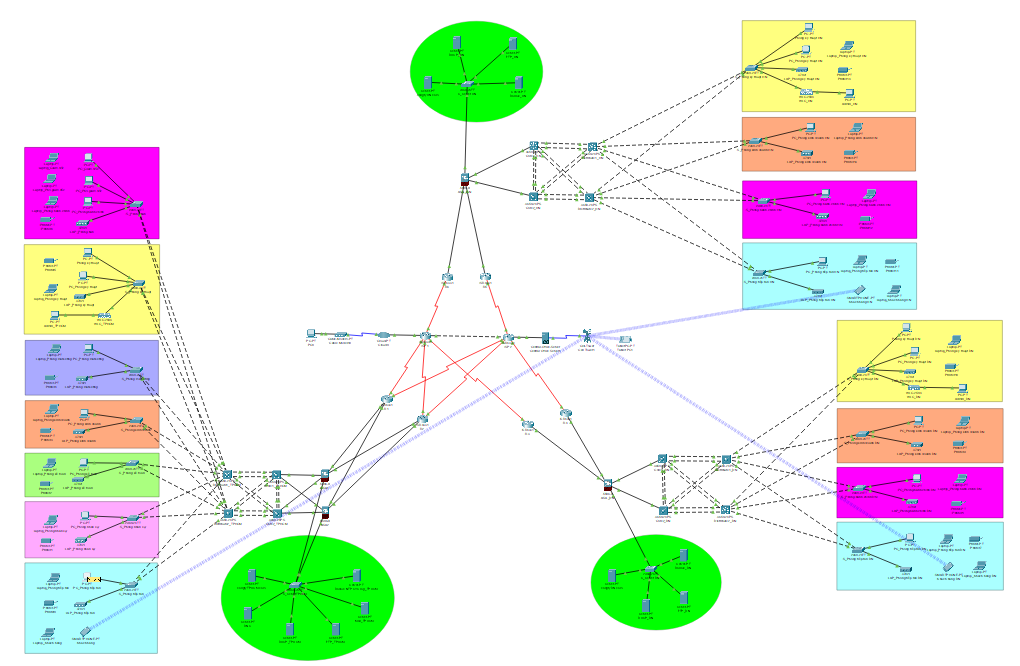
\includegraphics[width=16cm, height=12cm]{img/logic.png}
    \caption{Sơ đồ luận lý}
    \label{hinh21}
\end{figure}
\subsection{Sơ đồ vật lý}
\begin{figure}[H]
    \centering
    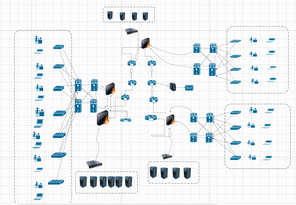
\includegraphics[width=16cm, height=12cm]{img/physical.png}
    \caption{Sơ đồ vật lý}
    \label{hinh22 }
\end{figure}
\subsection{Sơ đồ lắp đặt tủ Rack}
\begin{figure}[H]
    \centering
    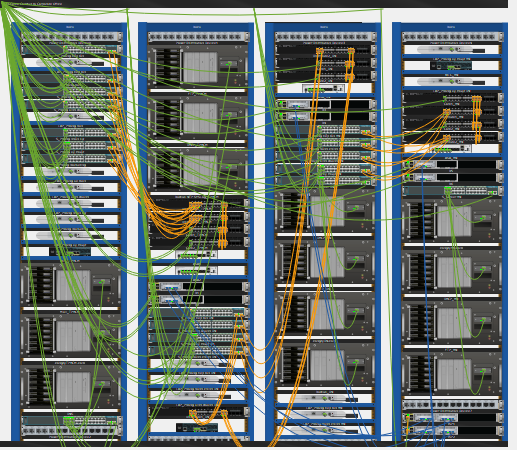
\includegraphics[width=16cm, height=14cm]{img/rack.png}
    \caption{Sơ đồ tủ Rack}
    \label{hinh23}
\end{figure}
\newpage


\section*{CHƯƠNG 3 - THÔNG TIN CÀI ĐẶT CẤU HÌNH HỆ THỐNG}
\addcontentsline{toc}{section}{\numberline{} CHƯƠNG 3 - THÔNG TIN CÀI ĐẶT CẤU HÌNH HỆ THỐNG}
\setcounter{section}{3}
\setcounter{subsection}{0}
\setcounter{figure}{0}
\setcounter{table}{0}
\subsection{Thông tin kết nối port trong hệ thống}
\begin{center}
\def\arraystretch{2.1}\begin{longtable}{|p{0.3\textwidth}|p{0.14\textwidth}|p{0.15\textwidth}|p{0.12\textwidth}|p{0.15 \textwidth}|}


\hline \textbf{Source to destination }    &      \textbf{Sources Interface }    &      \textbf{Destination Interface }    &    \textbf{Protocol } &     \textbf{Trunking/ vlan }\\ \hline
\endfirsthead



\hline \textbf{Source to destination } &  \textbf{Sources Interface } &  \textbf{Destination Interface } &  \textbf{Protocol } &  \textbf{Trunking/ vlan} \\ \hline
\endhead


\endfoot


\endlastfoot


\hline  S\_ServerTPHCM  to  congtyTPHCM\.com  &  Fa0/1  &  Fa0  &  Ethernet  &   \\
\hline  S\_ServerTPHCM  to  DNS  &  Fa0/2  &  Fa0  &  Ethernet  &   \\
\hline  S\_ServerTPHCM  to  DHCP\_TPHCM  &  Fa0/3  &  Fa0  &  Ethernet  &   \\
\hline  S\_ServerTPHCM  to  FTP\_TPHCM  &  Fa0/4  &  Fa0  &  Ethernet  &   \\
\hline  S\_ServerTPHCM  to  Mail\_TPHCM  &  Fa0/5  &  Fa0  &  Ethernet  &   \\
\hline  S\_ServerTPHCM  to  Radius NTP SYSLog\_TPHCM  &  Fa0/6  &  Fa0  &  Ethernet  &   \\
\hline  ASA1  to  S\_ServerTPHCM  &  G1/3  &  G0/1  &  Ethernet  &   \\
\hline  ASA1  to  R1  &  G1/4  &  G0/0/0  &  Ethernet  &   \\
\hline  ASA1  to  R2  &  G1/5  &  G0/0/0  &  Ethernet  &   \\
\hline  ASA1  to  Core1\_TPHCM  &  G1/1  &  G1/0/1  &  Ethernet  &   \\
\hline  ASA1  to  Core2\_TPHCM  &  G1/2  &  G1/0/2  &  Ethernet  &   \\
\hline  ASA2  to  S\_ServerTPHCM  &  G1/3  &  G0/2  &  Ethernet  &   \\
\hline  ASA2  to  R1  &  G1/4  &  G0/0/1  &  Ethernet  &   \\
\hline  ASA2  to  R2  &  G1/5  &  G0/0/1  &  Ethernet  &   \\
\hline  ASA2  to  Core1\_TPHCM  &  G1/2  &  G1/0/2  &  Ethernet  &   \\
\hline  ASA2  to  Core2\_TPHCM  &  G1/1  &  G1/0/1  &  Ethernet  &   \\
\hline  Core1\_TPHCM  to  Core2\_TPHCM  &  G1/0/19  &  G1/0/19  &  Ethernet  &  Port - Channel \\
\hline  Core1\_TPHCM  to  Core2\_TPHCM  &  G1/0/20  &  G1/0/20  &  Ethernet  &  Port - Channel \\
\hline  Core1\_TPHCM  to  Distribute1\_TPHCM  &  G1/0/23  &  G1/0/23  &  Ethernet  &  Port - Channel \\
\hline  Core1\_TPHCM  to  Distribute1\_TPHCM  &  G1/0/24  &  G1/0/24  &  Ethernet  &  Port - Channel \\
\hline  Core1\_TPHCM  to  Distribute2\_TPHCM  &  G1/0/21  &  G1/0/21  &  Ethernet  &  Port - Channel \\
\hline  Core1\_TPHCM  to  Distribute2\_TPHCM  &  G1/0/22  &  G1/0/22  &  Ethernet  &  Port - Channel \\
\hline  Core2\_TPHCM  to  Distribute1\_TPHCM  &  G1/0/21  &  G1/0/21  &  Ethernet  &  Port - Channel \\
\hline  Core2\_TPHCM  to  Distribute1\_TPHCM  &  G1/0/22  &  G1/0/22  &  Ethernet  &  Port - Channel \\
\hline  Core2\_TPHCM  to  Distribute2\_TPHCM  &  G1/0/23  &  G1/0/23  &  Ethernet  &  Port - Channel \\
\hline  Core2\_TPHCM  to  Distribute2\_TPHCM  &  G1/0/24  &  G1/0/24  &  Ethernet  &  Port - Channel \\
\hline  Distribute1\_TPHCM  to  S\_Phòng lễ Tân  &  G1/0/1  &  G0/1  &  Ethernet  &  TRUNKING \\
\hline  Distribute1\_TPHCM  to  S\_Phòng nhân sự  &  G1/0/2  &  G0/1  &  Ethernet  &  TRUNKING \\
\hline  Distribute1\_TPHCM  to  S\_Phòng kế toán  &  G1/0/3  &  G0/1  &  Ethernet  &  TRUNKING \\
\hline  Distribute1\_TPHCM  to  S\_Phòng kinh doanh  &  G1/0/4  &  G0/1  &  Ethernet  &  TRUNKING \\
\hline  Distribute1\_TPHCM  to  S\_Phòng marketing  &  G1/0/5  &  G0/1  &  Ethernet  &  TRUNKING \\
\hline  Distribute1\_TPHCM  to  S\_Phòng kỹ thuật  &  G1/0/6  &  G0/1  &  Ethernet  &  TRUNKING \\
\hline  Distribute1\_TPHCM  to  S\_Phòng ban  &  G1/0/7  &  G0/1  &  Ethernet  &  TRUNKING \\
\hline  Distribute2\_TPHCM  to  S\_Phòng tiếp tân  &  G1/0/1  &  G0/2  &  Ethernet  &  TRUNKING \\
\hline  Distribute2\_TPHCM  to  S\_Phòng nhân sự  &  G1/0/2  &  G0/2  &  Ethernet  &  TRUNKING \\
\hline  Distribute2\_TPHCM  to  S\_Phòng kế toán  &  G1/0/3  &  G0/2  &  Ethernet  &  TRUNKING \\
\hline  Distribute2\_TPHCM  to  S\_Phòng kinh doanh  &  G1/0/4  &  G0/2  &  Ethernet  &  TRUNKING \\
\hline  Distribute2\_TPHCM  to  S\_Phòng marketing  &  G1/0/5  &  G0/2  &  Ethernet  &  TRUNKING \\
\hline  Distribute2\_TPHCM  to  S\_Phòng kỹ thuật  &  G1/0/6  &  G0/2  &  Ethernet  &  TRUNKING \\
\hline  Distribute2\_TPHCM  to  S\_Phòng ban  &  G1/0/7  &  G0/2  &  Ethernet  &  TRUNKING \\
\hline  S\_Phòng tiếp tân  to  PC\_Phòng tiếp tân  &  Fa0/1  &  Fa0  &  Ethernet  &  VLAN \\
\hline  S\_Phòng nhân sự  to  PC\_Phòng nhân sự  &  Fa0/1  &  Fa0  &  Ethernet  &  VLAN \\
\hline  S\_Phòng kế toán  to  PC\_Phòng kế toán  &  Fa0/1  &  Fa0  &  Ethernet  &  VLAN \\
\hline  S\_Phòng kinh doanh  to  PC\_Phòng kinh doanh  &  Fa0/1  &  Fa0  &  Ethernet  &  VLAN \\
\hline  S\_Phòng marketing  to  PC\_Phòng marketing  &  Fa0/1  &  Fa0  &  Ethernet  &  VLAN \\
\hline  S\_Phòng kỹ thuật  to  Phòng kỹ thuật  &  Fa0/4  &  Fa0  &  Ethernet  &  VLAN \\
\hline  S\_Phòng kỹ thuật  to  PC\_Phòng kỹ thuật  &  Fa0/1  &  Fa0  &  Ethernet  &  VLAN \\
\hline  S\_Phòng kỹ thuật  to  WLC\_TPHCM  &  Fa0/3  &  G1  &  Ethernet  &  VLAN \\
\hline  WLC\_TPHCM  to  Admin\_TPHCM  &  G2  &  Fa0  &  Ethernet  &   \\
\hline  S\_Phòng ban  to  PC\_Giám đốc  &  Fa0/1  &  Fa0  &  Ethernet  &  VLAN \\
\hline  S\_Phòng ban  to  PC\_Phó giám đốc  &  Fa0/2  &  Fa0  &  Ethernet  &  VLAN \\
\hline  S\_Phòng ban  to  PC\_Phòng hành chính  &  Fa0/3  &  Fa0  &  Ethernet  &  VLAN \\
\hline  LAP\_Phòng tiếp tân  to  S\_Phòng tiếp tân  &  G0  &  Fa0/2  &  Ethernet  &  TRUNKING \\
\hline  LAP\_Phòng nhân sự  to  S\_Phòng nhân sự  &  G0  &  Fa0/2  &  Ethernet  &  TRUNKING \\
\hline  LAP\_Phòng kế toán  to  S\_Phòng kế toán  &  G0  &  Fa0/2  &  Ethernet  &  TRUNKING \\
\hline  LAP\_Phòng kinh doanh  to  S\_Phòng kinh doanh  &  G0  &  Fa0/2  &  Ethernet  &  TRUNKING \\
\hline  LAP\_Phòng marketing  to  S\_Phòng marketing  &  G0  &  Fa0/2  &  Ethernet  &  TRUNKING \\
\hline  LAP\_Phòng kỹ thuật  to  S\_Phòng kỹ thuật  &  G0  &  Fa0/2  &  Ethernet  &  TRUNKING \\
\hline  LAP\_Phòng ban  to  S\_Phòng ban  &  G0  &  Fa0/4  &  Ethernet  &  TRUNKING \\
\hline  LAP\_Phòng tiếp tân  to  Laptop\_Phòng tiếp tân  &    &    &  Wireless  &   \\
\hline  LAP\_Phòng tiếp tân  to  Laptop\_Khách hàng  &    &    &  Wireless  &   \\
\hline  LAP\_Phòng tiếp tân  to  Khách hàng  &    &    &  Wireless  &   \\
\hline  LAP\_Phòng tiếp tân  to  Printer0  &    &    &  Wireless  &   \\
\hline  LAP\_Phòng nhân sự  to  Laptop\_Phòng nhân sự  &    &    &  Wireless  &   \\
\hline  LAP\_Phòng nhân sự  to  Printer1  &    &    &  Wireless  &   \\
\hline  LAP\_Phòng kế toán  to  Laptop\_Phòng kế toán  &    &    &  Wireless  &   \\
\hline  LAP\_Phòng kế toán  to  Printer2  &    &    &  Wireless  &   \\
\hline  LAP\_Phòng kinh doanh  to  Laptop\_Phòng kinh doanh  &    &    &  Wireless  &   \\
\hline  LAP\_Phòng kinh doanh  to  Printer3  &    &    &  Wireless  &   \\
\hline  LAP\_Phòng marketing  to  Laptop\_Phòng marketing  &    &    &  Wireless  &   \\
\hline  LAP\_Phòng marketing  to  Printer4  &    &    &  Wireless  &   \\
\hline  LAP\_Phòng kỹ thuật  to  Laptop\_Phòng kỹ thuật  &    &    &  Wireless  &   \\
\hline  LAP\_Phòng kỹ thuật  to  Printer5  &    &    &  Wireless  &   \\
\hline  LAP\_Phòng ban  to  Laptop\_Giám đốc  &    &    &  Wireless  &   \\
\hline  LAP\_Phòng ban  to  Laptop\_Phó giám đốc  &    &    &  Wireless  &   \\
\hline  LAP\_Phòng ban  to  Laptop\_Phòng hành chính  &    &    &  Wireless  &   \\
\hline  LAP\_Phòng ban  to  Printer6  &    &    &  Wireless  &   \\
\hline  ISP1  to  R1  &  S0/1/0  &  S0/1/0  &    &   \\
\hline  ISP1  to  R3  &  S0/1/1  &  S0/1/0  &    &   \\
\hline  ISP1  to  R5  &  S0/2/0  &  S0/1/0  &    &   \\
\hline  ISP1  to  Cloud0  &  G0/0/1  &  Eth6  &  Ethernet  &   \\
\hline  ISP1  to  ISP2  &  G0/0/0  &  G0/0/0  &  Ethernet  &   \\
\hline  ISP2  to  R2  &  S0/1/0  &  S0/1/0  &    &   \\
\hline  ISP2  to  R4  &  S0/1/1  &  S0/1/0  &    &   \\
\hline  ISP2  to  R6  &  S0/2/0  &  S0/1/0  &    &   \\
\hline  ISP2  to  Central Office Server1  &  G0/0/1  &  Backbone  &  Ethernet  &   \\
\hline  Cable Modem0  to  Cloud0  &  Port0  &  Coaxial7  &    &   \\
\hline  Cable Modem0  to  PC0  &  Port1  &  Fa0  &  Ethernet  &   \\
\hline  S\_Server DN  to  congtyDN\.com  &  Fa0/1  &  Fa0  &  Ethernet  &   \\
\hline  S\_Server DN  to  DHCP\_DN  &  Fa0/2  &  Fa0  &  Ethernet  &   \\
\hline  S\_Server DN  to  FTP\_DN  &  Fa0/3  &  Fa0  &  Ethernet  &   \\
\hline  S\_Server DN  to  Radius\_DN  &  Fa0/4  &  Fa0  &  Ethernet  &   \\
\hline  ASA\_DN  to  S\_Server DN  &  G1/5  &  G0/1  &  Ethernet  &   \\
\hline  ASA\_DN  to  R3  &  G1/3  &  G0/0/0  &  Ethernet  &   \\
\hline  ASA\_DN  to  R4  &  G1/4  &  G0/0/0  &  Ethernet  &   \\
\hline  ASA\_DN  to  Core1\_DN  &  G1/1  &  G1/0/1  &  Ethernet  &   \\
\hline  ASA\_DN  to  Core2\_DN  &  G1/2  &  G1/0/1  &  Ethernet  &   \\
\hline  Core1\_DN  to  Core2\_DN  &  G1/0/19  &  G1/0/19  &  Ethernet  &  Port - Channel \\
\hline  Core1\_DN  to  Core2\_DN  &  G1/0/20  &  G1/0/20  &  Ethernet  &  Port - Channel \\
\hline  Core1\_DN  to  Distribute1\_DN  &  G1/0/23  &  G1/0/23  &  Ethernet  &  Port - Channel \\
\hline  Core1\_DN  to  Distribute1\_DN  &  G1/0/24  &  G1/0/24  &  Ethernet  &  Port - Channel \\
\hline  Core1\_DN  to  Distribute2\_DN  &  G1/0/21  &  G1/0/21  &  Ethernet  &  Port - Channel \\
\hline  Core1\_DN  to  Distribute2\_DN  &  G1/0/22  &  G1/0/22  &  Ethernet  &  Port - Channel \\
\hline  Core2\_DN  to  Distribute1\_DN  &  G1/0/21  &  G1/0/21  &  Ethernet  &  Port - Channel \\
\hline  Core2\_DN  to  Distribute1\_DN  &  G1/0/22  &  G1/0/22  &  Ethernet  &  Port - Channel \\
\hline  Core2\_DN  to  Distribute2\_DN  &  G1/0/23  &  G1/0/23  &  Ethernet  &  Port - Channel \\
\hline  Core2\_DN  to  Distribute2\_DN  &  G1/0/24  &  G1/0/24  &  Ethernet  &  Port - Channel \\
\hline  Distribute1\_DN  to  S\_Phòng tiếp tân DN  &  G1/0/1  &  G0/1  &  Ethernet  &  TRUNKING \\
\hline  Distribute1\_DN  to  S\_Phòng hành chính DN  &  G1/0/2  &  G0/1  &  Ethernet  &  TRUNKING \\
\hline  Distribute1\_DN  to  S\_Phòng kinh doanh DN  &  G1/0/3  &  G0/1  &  Ethernet  &  TRUNKING \\
\hline  Distribute1\_DN  to  S\_Phòng kỹ thuật DN  &  G1/0/4  &  G0/1  &  Ethernet  &  TRUNKING \\
\hline  Distribute2\_DN  to  S\_Phòng tiếp tân DN  &  G1/0/1  &  G0/2  &  Ethernet  &  TRUNKING \\
\hline  Distribute2\_DN  to  S\_Phòng hành chính DN  &  G1/0/2  &  G0/2  &  Ethernet  &  TRUNKING \\
\hline  Distribute2\_DN  to  S\_Phòng kinh doanh DN  &  G1/0/3  &  G0/2  &  Ethernet  &  TRUNKING \\
\hline  Distribute2\_DN  to  S\_Phòng kỹ thuật DN  &  G1/0/4  &  G0/2  &  Ethernet  &  TRUNKING \\
\hline  S\_Phòng tiếp tân DN  to  PC\_Phòng tiếp tân DN  &  Fa0/1  &  Fa0  &  Ethernet  &  VLAN \\
\hline  S\_Phòng hành chính DN  to  PC\_Phòng hành chính DN  &  Fa0/1  &  Fa0  &  Ethernet  &  VLAN \\
\hline  S\_Phòng kinh doanh DN  to  PC\_Phòng kinh doanh DN  &  Fa0/1  &  Fa0  &  Ethernet  &  VLAN \\
\hline  S\_Phòng kỹ thuật DN  to  Phòng kỹ thuật DN  &  Fa0/1  &  Fa0  &  Ethernet  &  VLAN \\
\hline  S\_Phòng kỹ thuật DN  to  PC\_Phòng kỹ thuật DN  &  Fa0/2  &  Fa0  &  Ethernet  &  VLAN \\
\hline  S\_Phòng kỹ thuật DN  to  WLC\_DN  &  Fa0/4  &  G1  &  Ethernet  &  VLAN \\
\hline  WLC\_DN  to  Admin\_DN  &  G2  &  Fa0  &  Ethernet  &   \\
\hline  LAP\_Phòng tiếp tân DN  to  Laptop\_Phòng tiếp tân DN  &    &    &  Wireless  &   \\
\hline  LAP\_Phòng tiếp tân DN  to  Laptop\_Khách hàng DN  &    &    &  Wireless  &   \\
\hline  LAP\_Phòng tiếp tân DN  to  Khách hàng DN  &    &    &  Wireless  &   \\
\hline  LAP\_Phòng tiếp tân DN  to  Printer7  &    &    &  Wireless  &   \\
\hline  LAP\_Phòng hành chính DN  to  Laptop\_Phòng hành chính DN  &    &    &  Wireless  &   \\
\hline  LAP\_Phòng hành chính DN  to  Printer8  &    &    &  Wireless  &   \\
\hline  LAP\_Phòng kinh doanh DN  to  Laptop\_Phòng kinh doanh DN  &    &    &  Wireless  &   \\
\hline  LAP\_Phòng kinh doanh DN  to  Printer9  &    &    &  Wireless  &   \\
\hline  LAP\_Phòng kỹ thuật DN  to  Laptop\_Phòng kỹ thuật DN  &    &    &  Wireless  &   \\
\hline  LAP\_Phòng kỹ thuật DN  to  Printer10  &    &    &  Wireless  &   \\
\hline  S\_Server HN  to  congtyHN\.com  &  Fa0/1  &  Fa0  &  Ethernet  &   \\
\hline  S\_Server HN  to  DHCP\_HN  &  Fa0/2  &  Fa0  &  Ethernet  &   \\
\hline  S\_Server HN  to  FTP\_HN  &  Fa0/3  &  Fa0  &  Ethernet  &   \\
\hline  S\_Server HN  to  Radius\_HN  &  Fa0/4  &  Fa0  &  Ethernet  &   \\
\hline  ASA\_HN  to  S\_Server HN  &  G1/5  &  G0/1  &  Ethernet  &   \\
\hline  ASA\_HN  to  R5  &  G1/3  &  G0/0/0  &  Ethernet  &   \\
\hline  ASA\_HN  to  R6  &  G1/4  &  G0/0/0  &  Ethernet  &   \\
\hline  ASA\_HN  to  Core1\_HN  &  G1/1  &  G1/0/1  &  Ethernet  &   \\
\hline  ASA\_HN  to  Core2\_HN  &  G1/2  &  G1/0/1  &  Ethernet  &   \\
\hline  Core1\_HN  to  Core2\_HN  &  G1/0/19  &  G1/0/19  &  Ethernet  &  Port - Channel \\
\hline  Core1\_HN  to  Core2\_HN  &  G1/0/20  &  G1/0/20  &  Ethernet  &  Port - Channel \\
\hline  Core1\_HN  to  Distribute1\_HN  &  G1/0/23  &  G1/0/23  &  Ethernet  &  Port - Channel \\
\hline  Core1\_HN  to  Distribute1\_HN  &  G1/0/24  &  G1/0/24  &  Ethernet  &  Port - Channel \\
\hline  Core1\_HN  to  Distribute2\_HN  &  G1/0/21  &  G1/0/21  &  Ethernet  &  Port - Channel \\
\hline  Core1\_HN  to  Distribute2\_HN  &  G1/0/22  &  G1/0/22  &  Ethernet  &  Port - Channel \\
\hline  Core2\_HN  to  Distribute1\_HN  &  G1/0/21  &  G1/0/21  &  Ethernet  &  Port - Channel \\
\hline  Core2\_HN  to  Distribute1\_HN  &  G1/0/22  &  G1/0/22  &  Ethernet  &  Port - Channel \\
\hline  Core2\_HN  to  Distribute2\_HN  &  G1/0/23  &  G1/0/23  &  Ethernet  &  Port - Channel \\
\hline  Core2\_HN  to  Distribute2\_HN  &  G1/0/24  &  G1/0/24  &  Ethernet  &  Port - Channel \\
\hline  Distribute1\_HN  to  S\_Phòng tiếp tân HN  &  G1/0/1  &  G0/1  &  Ethernet  &  TRUNKING \\
\hline  Distribute1\_HN  to  S\_Phòng hành chính HN  &  G1/0/2  &  G0/1  &  Ethernet  &  TRUNKING \\
\hline  Distribute1\_HN  to  S\_Phòng kinh doanh HN  &  G1/0/3  &  G0/1  &  Ethernet  &  TRUNKING \\
\hline  Distribute1\_HN  to  S\_Phòng kỹ thuật HN  &  G1/0/4  &  G0/1  &  Ethernet  &  TRUNKING \\
\hline  Distribute2\_HN  to  S\_Phòng tiếp tân HN  &  G1/0/1  &  G0/2  &  Ethernet  &  TRUNKING \\
\hline  Distribute2\_HN  to  S\_Phòng hành chính HN  &  G1/0/2  &  G0/2  &  Ethernet  &  TRUNKING \\
\hline  Distribute2\_HN  to  S\_Phòng kinh doanh HN  &  G1/0/3  &  G0/2  &  Ethernet  &  TRUNKING \\
\hline  Distribute2\_HN  to  S\_Phòng kỹ thuật HN  &  G1/0/4  &  G0/2  &  Ethernet  &  TRUNKING \\
\hline  S\_Phòng tiếp tân HN  to  PC\_Phòng tiếp tân HN  &  Fa0/1  &  Fa0  &  Ethernet  &   \\
\hline  S\_Phòng hành chính HN  to  PC\_Phòng hành chính HN  &  Fa0/1  &  Fa0  &  Ethernet  &   \\
\hline  S\_Phòng kinh doanh HN  to  PC\_Phòng kinh doanh HN  &  Fa0/1  &  Fa0  &  Ethernet  &   \\
\hline  S\_Phòng kỹ thuật HN  to  Phòng kỹ thuật HN  &  Fa0/1  &  Fa0  &  Ethernet  &   \\
\hline  S\_Phòng kỹ thuật HN  to  PC\_Phòng kỹ thuật HN  &  Fa0/2  &  Fa0  &  Ethernet  &   \\
\hline  S\_Phòng kỹ thuật HN  to  WLC\_HN  &  Fa0/4  &  G1  &  Ethernet  &   \\
\hline  WLC\_HN  to  Admin\_HN  &  G2  &  Fa0  &  Ethernet  &   \\
\hline  LAP\_Phòng tiếp tân HN  to  Laptop\_Phòng tiếp tân HN  &    &    &  Wireless  &   \\
\hline  LAP\_Phòng tiếp tân HN  to  Laptop\_Khách hàng HN  &    &    &  Wireless  &   \\
\hline  LAP\_Phòng tiếp tân HN  to  Khách hàng HN  &    &    &  Wireless  &   \\
\hline  LAP\_Phòng tiếp tân HN  to  Printer11  &    &    &  Wireless  &   \\
\hline  LAP\_Phòng hành chính HN  to  Laptop\_Phòng hành chính HN  &    &    &  Wireless  &   \\
\hline  LAP\_Phòng hành chính HN  to  Printer12  &    &    &  Wireless  &   \\
\hline  LAP\_Phòng kinh doanh HN  to  Laptop\_Phòng kinh doanh HN  &    &    &  Wireless  &   \\
\hline  LAP\_Phòng kinh doanh HN  to  Printer13  &    &    &  Wireless  &   \\
\hline  LAP\_Phòng kỹ thuật HN  to  Laptop\_Phòng kỹ thuật HN  &    &    &  Wireless  &   \\
\hline  LAP\_Phòng kỹ thuật HN  to  Printer14  &    &    &  Wireless  &   \\
\hline


    \caption{Thông tin kết nối port trong hệ thống}
    \label{hinh31}
\end{longtable}

\end{center}



\subsection{Thông tin VLAN, Interface VLAN trong hệ thống}
\begin{center}
\def\arraystretch{2.1}\begin{longtable}{|p{0.05\textwidth}|p{0.17\textwidth}|p{0.08\textwidth}|p{0.1\textwidth}|p{0.06\textwidth}|p{0.16\textwidth}|p{0.28\textwidth}|}


\hline \textbf{STT } &  \textbf{VLAN Name } &  \textbf{VLAN ID } &  \textbf{Phòng Ban } &  \textbf{Mask} &  \textbf{Default gateway } &  \textbf{Ipv6} \\ \hline
\endfirsthead


\endhead


\endfoot


\endlastfoot

\hline  1  &  TIEPTAN  &  10  &  Tiếp tân  &  /28  &  192.168.10.1  &  2001:db8:acad:a::1/64 \\
\hline  2  &  NHANSU  &  11  &  Nhân sự  &  /25  &  192.168.11.1  &  2001:db8:acad:b::1/64 \\
\hline  3  &  KETOAN  &  12  &  Kế toán  &  /28  &  192.168.12.1  &  2001:db8:acad:c::1/64 \\
\hline  4  &  KINH DOANH  &  13  &  Kinh doanh  &  /25  &  192.168.13.1  &  2001:db8:acad:d::1/64 \\
\hline  5  &  MARKETING  &  14  &  Marketing  &  /26  &  192.168.14.1  &  2001:db8:acad:e::1/64 \\
\hline  6  &  KYTHUAT  &  15  &  Kỹ thuật  &  /27  &  192.168.15.1  &  2001:db8:acad:f::1/64 \\
\hline  7  &  HANH CHINH  &  16  &  Hành chính  &  /26  &  192.168.16.1  &  2001:db8:acad:16::1/64 \\
\hline  8  &  GIAMDOC  &  17  &  Giám đốc  &  /29  &  192.168.17.1  &  2001:db8:acad:17::1/64 \\
\hline  9  &  PHOGIAM DOC  &  18  &  Phó giám đốc  &  /29  &  192.168.18.1  &  2001:db8:acad:18::1/64 \\
\hline  10  &  KHACH HANG  &  100  &  Khách hàng  &  /24  &  200.200.100.1  &  2001:db8:acad:100::1/64 \\
\hline  11  &  TIEPTAN \_DN  &  19  &  Tiếp tân  &  /29  &  192.168.19.1  &  2001:db8:acad:19::1/64 \\
\hline  12  &  HANH CHINH \_DN  &  20  &  Hành chính  &  /27  &  192.168.20.1  &  2001:db8:acad:20::1/64 \\
\hline  13  &  KINH DOANH \_DN  &  21  &  Kinh doanh  &  /26  &  192.168.21.1  &  2001:db8:acad:21::1/64 \\
\hline  14  &  KYTHUAT \_DN  &  22  &  Kỹ thuật  &  /28  &  192.168.22.1  &  2001:db8:acad:22::1/64 \\
\hline  15  &  KHACH HANG \_DN  &  150  &  Khách hàng  &  /24  &  200.200.150.1  &  2001:db8:acad:150::1/64 \\
\hline  16  &  TIEPTAN \_HN  &  23  &  Tiếp tân  &  /29  &  192.168.23.1  &  2001:db8:acad:23::1/64 \\
\hline  17  &  HANH CHINH \_HN  &  24  &  Hành chính  &  /27  &  192.168.24.1  &  2001:db8:acad:24::1/64 \\
\hline  18  &  KINH DOANH \_HN  &  25  &  Kinh doanh  &  /26  &  192.168.25.1  &  2001:db8:acad:25::1/64 \\
\hline  19  &  KYTHUAT \_HN  &  26  &  Kỹ thuật  &  /28  &  192.168.26.1  &  2001:db8:acad:26::1/64 \\
\hline  20  &  KHACH HANG \_HN  &  200  &  Khách hàng  &  /24  &  200.200.200.1  &  2001:db8:acad:200::1/64 \\
 
 
\hline
   \caption{Thông tin VLAN, interface VLAN trong hệ thống}
    \label{hinh33}\\
\end{longtable}
   
\end{center}



\subsection{Thông tin thiết kế quy hoạch địa chỉ IP Planning}
\begin{center}
    \def\arraystretch{2.1}\begin{longtable}{|p{0.04\textwidth}|p{0.1\textwidth}|p{0.09\textwidth}|p{0.185\textwidth}|p{0.04\textwidth}|p{0.175\textwidth}|p{0.30\textwidth}|}
    
    
    \hline \textbf{ST T} &\textbf{DE- VICES} & \textbf{INTER FACE} &  \textbf{IPv4 ADDRESS} &  \textbf{Ma- sk} &\textbf{NET} & \textbf{IPV6}\\ \hline 
    
    \endfirsthead
    
    
    
    \hline \textbf{ST T} &\textbf{DE- VICES} & \textbf{INTER FACE} &  \textbf{IPv4 ADDRESS} &  \textbf{Ma- sk} &\textbf{NET} & \textbf{IPV6}\\ \hline 
    
    \endhead
    
       
    \endfoot
    
    
    \endlastfoot
        \hline  \multicolumn{7}{|c|}{I/Router biên và internet} \\
        \hline  1  &  ISP1  &  G0/0/0  &  209.100.100.100  &  /24  &  209.100.100.0  &  2001:db8:acad:227::1/64 \\
\hline  2  &  ISP1  &  G0/0/1  &  209.165.200.100  &  /24  &  209.165.200.0  &  2001:db8:acad:228::1/64 \\
\hline  3  &  ISP1  &  S0/1/0  &  209.165.100.1  &  /30  &  209.165.100.0  &  2001:db8:acad:209::1/64 \\
\hline  4  &  ISP1  &  S0/1/1  &  209.165.100.9  &  /30  &  209.165.100.8  &  2001:db8:acad:210::1/64 \\
\hline  5  &  ISP1  &  S0/2/0  &  209.165.100.21  &  /30  &  209.165.100.20  &  2001:db8:acad:214::1/64 \\
\hline  6  &  ISP1  &  S0/2/1  &  209.165.100.30  &  /30  &  209.165.100.28  &  2001:db8:acad:225::1/64 \\
\hline  7  &  ISP2  &  G0/0/0  &  209.100.100.200  &  /24  &  209.100.100.0  &  2001:db8:acad:227::2/64 \\
\hline  8  &  ISP2  &  G0/0/1  &  209.100.200.200  &  /24  &  209.100.200.0  &  2001:db8:acad:229::1/64 \\
\hline  9  &  ISP2  &  S0/1/0  &  209.165.100.5  &  /30  &  209.165.100.4  &  2001:db8:acad:211::1/64 \\
\hline  10  &  ISP2  &  S0/1/1  &  209.165.100.13  &  /30  &  209.165.100.12  &  2001:db8:acad:212::1/64 \\
\hline  11  &  ISP2  &  S0/2/0  &  209.165.100.17  &  /30  &  209.165.100.16  &  2001:db8:acad:213::1/64 \\
\hline  12  &  ISP2  &  S0/2/1  &  209.165.100.26  &  /30  &  209.165.100.24  &  2001:db8:acad:226::1/64 \\
\hline  13  &  R1  &  G0/0/0  &  172.16.0.89  &  /30  &  172.16.0.88  &  2001:db8:acad:172::1/64 \\
\hline  14  &  R1  &  G0/0/1  &  172.16.0.73  &  /30  &  172.16.0.72  &  2001:db8:acad:177::1/64 \\
\hline  15  &  R1  &  S0/1/0  &  209.165.100.2  &  /30  &  209.165.100.0  &  2001:db8:acad:209::2/64 \\
\hline  16  &  R1  &  S0/1/1  &  209.165.100.25  &  /30  &  209.165.100.24  &  2001:db8:acad:226::2/64 \\
\hline  17  &  R2  &  G0/0/0  &  172.16.0.5  &  /30  &  172.16.0.4  &  2001:db8:acad:173::1/64 \\
\hline  18  &  R2  &  G0/0/1  &  172.16.0.77  &  /30  &  172.16.0.76  &  2001:db8:acad:178::1/64 \\
\hline  19  &  R2  &  S0/1/0  &  209.165.100.6  &  /30  &  209.165.100.4  &  2001:db8:acad:211::2/64 \\
\hline  20  &  R2  &  S0/1/1  &  209.165.100.29  &  /30  &  209.165.100.28  &  2001:db8:acad:225::2/64 \\
\hline  21  &  R3  &  G0/0/0  &  172.16.0.33  &  /30  &  172.16.0.32  &  2001:db8:acad:186::1/64 \\
\hline  22  &  R3  &  S0/1/0  &  209.165.100.10  &  /30  &  209.165.100.8  &  2001:db8:acad:210::2/64 \\
\hline  23  &  R4  &  G0/0/0  &  172.16.0.37  &  /30  &  172.16.0.36  &  2001:db8:acad:187::1/64 \\
\hline  24  &  R4  &  S0/1/0  &  209.165.100.14  &  /30  &  209.165.100.12  &  2001:db8:acad:212::2/64 \\
\hline  25  &  R5  &  G0/0/0  &  172.16.0.93  &  /30  &  172.16.0.92  &  2001:db8:acad:217::1/64 \\
\hline  26  &  R5  &  S0/1/0  &  209.165.100.18  &  /30  &  209.165.100.16  &  2001:db8:acad:213::2/64 \\
\hline  27  &  R6  &  G0/0/0  &  172.16.0.97  &  /30  &  172.16.0.96  &  2001:db8:acad:218::1/64 \\
\hline  28  &  R6  &  S0/1/0  &  209.165.100.22  &  /30  &  209.165.100.20  &  2001:db8:acad:214::2/64 \\
\hline  29  &  PC0  &  Fa0  &  209.165.200.200  &  /24  &  209.165.200.0  &  <not set> \\
			
        \hline  \multicolumn{7}{|c|}{II/TPHCM} \\
        \hline  1  &  ASA1  &  G1/1  &  172.16.0.9  &  /30  &  172.16.0.8  &  2001:db8:acad:174::1/64 \\
\hline  2  &  ASA1  &  G1/2  &  172.16.0.13  &  /30  &  172.16.0.12  &  2001:db8:acad:175::1/64 \\
\hline  3  &  ASA1  &  G1/3  &  10.10.10.1  &  /28  &  10.10.10.0  &  2001:db8:badc:a::1/64 \\
\hline  4  &  ASA1  &  G1/4  &  172.16.0.90  &  /30  &  172.16.0.88  &  2001:db8:acad:172::2/64 \\
\hline  5  &  ASA1  &  G1/5  &  172.16.0.6  &  /30  &  172.16.0.4  &  2001:db8:acad:173::2/64 \\
\hline  6  &  ASA2  &  G1/1  &  172.16.0.81  &  /30  &  172.16.0.80  &  2001:db8:acad:180::1/64 \\
\hline  7  &  ASA2  &  G1/2  &  172.16.0.85  &  /30  &  172.16.0.84  &  2001:db8:acad:179::1/64 \\
\hline  8  &  ASA2  &  G1/3  &  10.10.10.8  &  /28  &  10.10.10.0  &  2001:db8:badc:a::1/64 \\
\hline  9  &  ASA2  &  G1/4  &  172.16.0.74  &  /30  &  172.16.0.72  &  2001:db8:acad:177::2/64 \\
\hline  10  &  ASA2  &  G1/5  &  172.16.0.78  &  /30  &  172.16.0.76  &  2001:db8:acad:178::2/64 \\
\hline  11  &  congty TPHCM .com  &  Fa0  &  10.10.10.2  &  /28  &  10.10.10.0  &  2001:db8:badc:a::2/64 \\
\hline  12  &  DNS  &  Fa0  &  10.10.10.3  &  /28  &  10.10.10.0  &  2001:db8:badc:a::3/64 \\
\hline  13  &  DHCP \_TP HCM  &  Fa0  &  10.10.10.4  &  /28  &  10.10.10.0  &  2001:db8:badc:a::4/64 \\
\hline  14  &  FTP \_TP HCM  &  Fa0  &  10.10.10.5  &  /28  &  10.10.10.0  &  2001:db8:badc:a::5/64 \\
\hline  15  &  Mail \_TP HCM  &  Fa0  &  10.10.10.6  &  /28  &  10.10.10.0  &  2001:db8:badc:a::6/64 \\
\hline  16  &  Radius NTP SYSLog \_TP HCM  &  Fa0  &  10.10.10.7  &  /28  &  10.10.10.0  &  2001:db8:badc:a::7/64 \\
\hline  17  &  Core1 \_TP HCM  &  G1/0/1  &  172.16.0.10  &  /30  &  172.16.0.8  &  2001:db8:acad:174::2/64 \\
\hline  18  &  Core1 \_TP HCM  &  G1/0/2  &  172.16.0.86  &  /30  &  172.16.0.84  &  2001:db8:acad:179::2/64 \\
\hline  19  &  Core1 \_TP HCM  &  G1/0/19-20(Port 1)  &  172.16.0.65  &  /30  &  172.16.0.64  &  2001:db8:acad:185::1/64 \\
\hline  20  &  Core1 \_TP HCM  &  G1/0/23-24(Port 2)  &  172.16.0.17  &  /30  &  172.16.0.16  &  2001:db8:acad:181::1/64 \\
\hline  21  &  Core1 \_TP HCM  &  G1/0/21-22(Port 3)  &  172.16.0.21  &  /30  &  172.16.0.20  &  2001:db8:acad:182::1/64 \\
\hline  22  &  Core2 \_TP HCM  &  G1/0/1  &  172.16.0.82  &  /30  &  172.16.0.80  &  2001:db8:acad:180::2/64 \\
\hline  23  &  Core2 \_TP HCM  &  G1/0/2  &  172.16.0.14  &  /30  &  172.16.0.12  &  2001:db8:acad:175::2/64 \\
\hline  24  &  Core2 \_TP HCM  &  G1/0/19-20(Port 1)  &  172.16.0.66  &  /30  &  172.16.0.64  &  2001:db8:acad:185::2/64 \\
\hline  25  &  Core2 \_TP HCM  &  G1/0/23-24(Port 2)  &  172.16.0.29  &  /30  &  172.16.0.28  &  2001:db8:acad:184::1/64 \\
\hline  26  &  Core2 \_TP HCM  &  G1/0/21-22(Port 3)  &  172.16.0.25  &  /30  &  172.16.0.24  &  2001:db8:acad:183::1/64 \\
\hline  27  &  Distri- bute1 \_TP HCM  &  G1/0/23-24(Port 2)  &  172.16.0.18  &  /30  &  172.16.0.16  &  2001:db8:acad:181::2/64 \\
\hline  28  &  Distri- bute1 \_TP HCM  &  G1/0/21-22(Port 3)  &  172.16.0.26  &  /30  &  172.16.0.24  &  2001:db8:acad:183::2/64 \\
\hline  29  &  Distri- bute1 \_TP HCM  &  G1/0/1-7  &    \multicolumn{4}{|c|}{Trunking/Passive Interface} \\
\hline  30  &  Distri- bute2 \_TP HCM  &  G1/0/23-24(Port 2)  &  172.16.0.30  &  /30  &  172.16.0.28  &  2001:db8:acad:184::2/64 \\
\hline  31  &  Distri- bute2 \_TP HCM  &  G1/0/21-22(Port 3)  &  172.16.0.22  &  /30  &  172.16.0.20  &  2001:db8:acad:182::2/64 \\
\hline  32  &  Distri- bute2 \_TP HCM  &  G1/0/1-7  &    \multicolumn{4}{|c|}{Trunking/Passive Interface} \\
		
        \hline  \multicolumn{7}{|c|}{III/Đà Nẵng} \\
        \hline \multirow{5}{*}{1} &  ASA \_DN  &  G1/1  &  172.16.0.41  &  /30  &  172.16.0.40  &  2001:db8:acad:188::1/64 \\\cline{3-7}		                          &    &  G1/2  &  172.16.0.45  &  /30  &  172.16.0.44  &  2001:db8:acad:189::1/64\\\cline{3-7}	                          		                          &    &  G1/3  &  172.16.0.34  &  /30  &  172.16.0.32  &  2001:db8:acad:186::2/64\\\cline{3-7}                                             		                          &    &  G1/3  &  172.16.0.34  &  /30  &  172.16.0.32  &  2001:db8:acad:186::2/64\\\cline{3-7}                 		                          &    &  G1/5  &  10.10.11.1  &  /28  &  10.10.11.0  &  2001:db8:badc:b::1/64\\\cline{3-7}
        
        \hline  2  &  congty DN.com  &  Fa0  &  10.10.11.2  &  /28  &  10.10.11.0  &  2001:db8:badc:b::2/64 \\
\hline  3  &  DHCP \_DN  &  Fa0  &  10.10.11.3  &  /28  &  10.10.11.0  &  2001:db8:badc:b::3/64 \\
\hline  4  &  FTP \_DN  &  Fa0  &  10.10.11.4  &  /28  &  10.10.11.0  &  2001:db8:badc:b::4/64 \\
\hline  5  &  Radius \_DN  &  Fa0  &  10.10.11.5  &  /28  &  10.10.11.0  &  2001:db8:badc:b::5/64 \\

\hline  \multirow{4}{*}{6}  &  Core1 \_DN  &  G1/0/1  &  172.16.0.42  &  /30  &  172.16.0.40  &  2001:db8:acad:188::2/64 \\\cline{3-7}
&    &  G1/0/19-20(Port 1)  &  172.16.0.69  &  /30  &  172.16.0.68  &  2001:db8:acad:194::1/64 \\\cline{3-7}
&    &  G1/0/23-24(Port 2)  &  172.16.0.49  &  /30  &  172.16.0.48  &  2001:db8:acad:190::1/64 \\\cline{3-7}
&    &  G1/0/21-22(Port 3)  &  172.16.0.53  &  /30  &  172.16.0.52  &  2001:db8:acad:191::1/64 \\\cline{3-7}

\hline  \multirow{4}{*}{7}  &  Core2 \_DN  &  G1/0/1  &  172.16.0.46  &  /30  &  172.16.0.44  &  2001:db8:acad:189::2/64 \\\cline{3-7}
&    &  G1/0/19-20(Port 1)  &  172.16.0.70  &  /30  &  172.16.0.68  &  2001:db8:acad:194::2/64 \\\cline{3-7}
&    &  G1/0/23-24(Port 2)  &  172.16.0.61  &  /30  &  172.16.0.60  &  2001:db8:acad:193::1/64 \\\cline{3-7}
&    &  G1/0/21-22(Port 3)  &  172.16.0.57  &  /30  &  172.16.0.56  &  2001:db8:acad:192::1/64 \\\cline{3-7}

\hline  \multirow{3}{*}{8}  &  Distri- bute1 \_DN  &  G1/0/23-24(Port 2)  &  172.16.0.50  &  /30  &  172.16.0.48  &  2001:db8:acad:190::2/64 \\\cline{3-7}
&    &  G1/0/21-22(Port 3)  &  172.16.0.58  &  /30  &  172.16.0.56  &  2001:db8:acad:192::2/64 \\\cline{3-7}
&    &  G1/0/1-4  &    \multicolumn{4}{|c|}{Trunking/Passive Interface} \\\cline{3-7}

\hline  \multirow{3}{*}{8}  &  Distri- bute2 \_DN  &  G1/0/23-24(Port 2)  &  172.16.0.62  &  /30  &  172.16.0.60  &  2001:db8:acad:193::2/64 \\\cline{3-7}
&     &  G1/0/21-22(Port 3)  &  172.16.0.54  &  /30  &  172.16.0.52  &  2001:db8:acad:191::2/64 \\\cline{3-7}
&     &  G1/0/1-4  &    \multicolumn{4}{|c|}{Trunking/Passive Interface} \\\cline{3-7}


\hline  \multicolumn{7}{|c|}{IV/Hà Nội} \\
        \hline \multirow{5}{*}{1} &  ASA \_HN  &  G1/1  &  172.16.0.101  &  /30  &  172.16.0.100  &  2001:db8:acad:215::1/64  \\\cline{3-7}		                          &    &  G1/2  &  172.16.0.105  &  /30  &  172.16.0.104  &  2001:db8:acad:216::1/64\\\cline{3-7}	                          		                          &     &  G1/3  &  172.16.0.94  &  /30  &  172.16.0.92  &  2001:db8:acad:217::2/64\\\cline{3-7}                                             		                          &    &  G1/4  &  172.16.0.98  &  /30  &  172.16.0.96  &  2001:db8:acad:218::2/64\\\cline{3-7}                 		                          &     &  G1/5  &  10.10.12.1  &  /28  &  10.10.12.0  &  2001:db8:badc:c::1/64\\\cline{3-7}
        
        \hline  2  &  congty HN.com  &  Fa0  &  10.10.12.2  &  /28  &  10.10.12.0  &  2001:db8:badc:c::2/64  \\
\hline  3  &  DHCP \_HN  &  Fa0  &  10.10.12.3  &  /28  &  10.10.12.0  &  2001:db8:badc:c::3/64 \\
\hline  4  &  FTP \_HN  &  Fa0  &  10.10.12.4  &  /28  &  10.10.12.0  &  2001:db8:badc:c::4/64  \\
\hline  5  &  Radius \_HN  &  Fa0  &  10.10.12.5  &  /28  &  10.10.12.0  &  2001:db8:badc:c::5/64 \\

\hline  \multirow{4}{*}{6}  &  Core1 \_HN  &  G1/0/1  &  172.16.0.102  &  /30  &  172.16.0.100  &  2001:db8:acad:215::2/64  \\\cline{3-7}
&    &  G1/0/19-20(Port 1)  &  172.16.0.109  &  /30  &  172.16.0.108  &  2001:db8:acad:219::1/64 \\\cline{3-7}
&    &  G1/0/23-24(Port 2)  &  172.16.0.113  &  /30  &  172.16.0.112  &  2001:db8:acad:220::1/64 \\\cline{3-7}
&    &  G1/0/21-22(Port 3)  &  172.16.0.117  &  /30  &  172.16.0.116  &  2001:db8:acad:221::1/64 \\\cline{3-7}

\hline  \multirow{4}{*}{7}  &  Core2 \_HN  &  G1/0/1  &  172.16.0.106  &  /30  &  172.16.0.104  &  2001:db8:acad:216::2/64 \\\cline{3-7}
&     &  G1/0/19-20(Port 1)  &  172.16.0.110  &  /30  &  172.16.0.108  &  2001:db8:acad:219::2/64 \\\cline{3-7}
&     &  G1/0/23-24(Port 2)  &  172.16.0.121  &  /30  &  172.16.0.120  &  2001:db8:acad:223::1/64 \\\cline{3-7}
&    &  G1/0/21-22(Port 3)  &  172.16.0.125  &  /30  &  172.16.0.124  &  2001:db8:acad:224::1/64 \\\cline{3-7}

\hline  \multirow{3}{*}{8}  &  Distri- bute1 \_HN  &  G1/0/23-24(Port 2)  &  172.16.0.114  &  /30  &  172.16.0.112  &  2001:db8:acad:220::2/64\\\cline{3-7}
&    &  G1/0/21-22(Port 3)  &  172.16.0.126  &  /30  &  172.16.0.124  &  2001:db8:acad:224::2/64 \\\cline{3-7}
&    &  G1/0/1-4   &    \multicolumn{4}{|c|}{Trunking/Passive Interface} \\\cline{3-7}

\hline  \multirow{3}{*}{8}  &  Distri- bute2 \_HN  &  G1/0/23-24(Port 2)  &  172.16.0.122  &  /30  &  172.16.0.120  &  2001:db8:acad:223::2/64 \\\cline{3-7}
&     &  G1/0/21-22(Port 3)  &  172.16.0.118  &  /30  &  172.16.0.116  &  2001:db8:acad:221::2/64 \\\cline{3-7}
&     &  G1/0/1-4  &    \multicolumn{4}{|c|}{Trunking/Passive Interface} \\\cline{3-7}

	
\hline  \multicolumn{7}{|c|}{V/ VPN tunel} \\	                          
\hline  1  &  R1  &  tunnel1  &  192.168.1.1  &  /30  &  192.168.1.0  &  <not set> \\
\hline  2  &  R1  &  tunnel2  &  192.168.1.5  &  /30  &  192.168.1.4  &  <not set> \\
\hline  3  &  R3  &  tunnel1  &  192.168.1.2  &  /30  &  192.168.1.0  &  <not set> \\
\hline  4  &  R5  &  tunnel1  &  192.168.1.6  &  /30  &  192.168.1.4  &  <not set> \\
\hline  5  &  R2  &  tunnel1  &  192.168.2.1  &  /30  &  192.168.2.0  &  <not set> \\
\hline  6  &  R2  &  tunnel2  &  192.168.2.5  &  /30  &  192.168.2.4  &  <not set> \\
\hline  7  &  R4  &  tunnel1  &  192.168.2.2  &  /30  &  192.168.2.0  &  <not set> \\
\hline  8  &  R6  &  tunnel1  &  192.168.2.6  &  /30  &  192.168.2.4  &  <not set> \\
        \hline
        \caption{Thông tin thiết kế quy hoạch địa chỉ IP planning}
        \label{hinh33a }
    \end{longtable}
    
    \end{center}
\newpage
\section*{CHƯƠNG 4 - CẤU HÌNH HẠ TẦNG}
\addcontentsline{toc}{section}{\numberline{} CHƯƠNG 4 - CẤU HÌNH HẠ TẦNG}
\setcounter{section}{4}
\setcounter{subsection}{0}
\setcounter{figure}{0}
\setcounter{table}{0}
\subsection{Cấu hình Interface}
\subsubsection{Khu vực Router biên và Internet}
\begin{figure}[H]
    \centering
    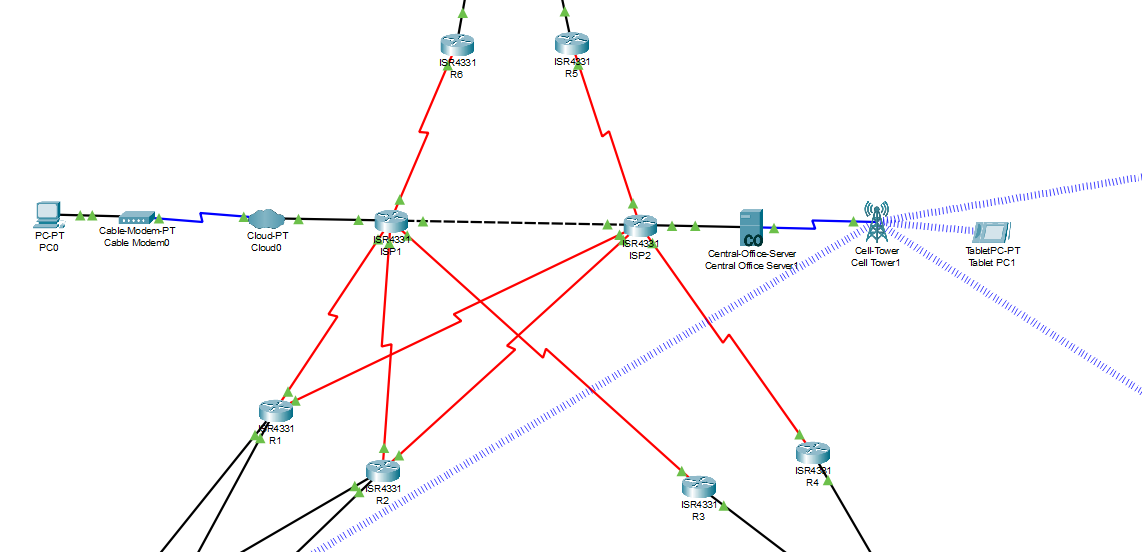
\includegraphics[width=16cm, height=6cm]{img/router.png}
    \caption{Khu vực Router biên và Internet}
    \label{hinh41}
\end{figure}
\textbf{a. Router R1} \\
\hspace*{2cm}\textit{interface G0/0/0\\
\hspace*{2cm}ip address 172.16.0.89 255.255.255.252\\
\hspace*{2cm}ipv6 address 2001:db8:acad:172::1/64\\
\hspace*{2cm}ip nat in\\
\hspace*{2cm}no shutdown\\
\hspace*{2cm}interface G0/0/1\\
\hspace*{2cm}ip address 172.16.0.73 255.255.255.252\\
\hspace*{2cm}ipv6 address 2001:db8:acad:177::1/64\\
\hspace*{2cm}ip nat in\\
\hspace*{2cm}no shutdown\\
\hspace*{2cm}interface S0/1/0\\
\hspace*{2cm}ip address 209.165.100.2 255.255.255.252\\
\hspace*{2cm}ipv6 address 2001:db8:acad:209::2/64\\
\hspace*{2cm}ip nat out\\
\hspace*{2cm}clock rate 2000000 \\
\hspace*{2cm}no shutdown\\
\hspace*{2cm}interface S0/1/1\\
\hspace*{2cm}ip address 209.165.100.25 255.255.255.252\\
\hspace*{2cm}ipv6 address 2001:db8:acad:226::2/64\\
\hspace*{2cm}ip nat out\\
\hspace*{2cm}no shutdown\\
\hspace*{2cm}interface Tunnel 1\\
\hspace*{2cm}ip address 192.168.1.1 255.255.255.252\\
\hspace*{2cm}tunnel mode gre ip\\
\hspace*{2cm}tunnel source S0/1/0\\
\hspace*{2cm}tunnel destination 209.165.100.10\\
\hspace*{2cm}no shutdown\\
\hspace*{2cm}interface Tunnel 2\\
\hspace*{2cm}ip address 192.168.1.5 255.255.255.252\\
\hspace*{2cm}tunnel mode gre ip\\
\hspace*{2cm}tunnel source S0/1/1\\
\hspace*{2cm}tunnel destination 209.165.100.18\\
\hspace*{2cm}no shutdown\\}
\hspace*{1cm}\textbf{b.Router R2} \\
\hspace*{2cm}\textit{interface G0/0/0\\
\hspace*{2cm}ip address 172.16.0.5 255.255.255.252\\
\hspace*{2cm}ipv6 address 2001:db8:acad:173::1/64\\
\hspace*{2cm}ip nat in\\
\hspace*{2cm}no shutdown\\
\hspace*{2cm}interface G0/0/1\\
\hspace*{2cm}ip address 172.16.0.77 255.255.255.252\\
\hspace*{2cm}ipv6 address 2001:db8:acad:178::1/64\\
\hspace*{2cm}ip nat in\\
\hspace*{2cm}no shutdown\\
\hspace*{2cm}interface S0/1/0\\
\hspace*{2cm}ip address 209.165.100.6 255.255.255.252\\
\hspace*{2cm}ipv6 address 2001:db8:acad:211::2/64\\
\hspace*{2cm}ip nat out\\
\hspace*{2cm}clock rate 2000000 \\
\hspace*{2cm}no shutdown\\
\hspace*{2cm}interface S0/1/1\\
\hspace*{2cm}ip address 209.165.100.29 255.255.255.252\\
\hspace*{2cm}ipv6 address 2001:db8:acad:225::2/64\\
\hspace*{2cm}ip nat out\\
\hspace*{2cm}no shutdown\\
\hspace*{2cm}interface Tunnel 1\\
\hspace*{2cm}ip address 192.168.2.1 255.255.255.252\\
\hspace*{2cm}tunnel mode gre ip\\
\hspace*{2cm}tunnel source S0/1/0\\
\hspace*{2cm}tunnel destination 209.165.100.14\\
\hspace*{2cm}no shutdown\\
\hspace*{2cm}interface Tunnel 2\\
\hspace*{2cm}ip address 192.168.2.5 255.255.255.252\\
\hspace*{2cm}tunnel mode gre ip\\
\hspace*{2cm}tunnel source S0/1/1\\
\hspace*{2cm}tunnel destination 209.165.100.22\\
\hspace*{2cm}no shutdown\\}
\hspace*{1cm}\textbf{c.Router R3} \\
\hspace*{2cm}\textit{interface G0/0/0\\
\hspace*{2cm}ip address 172.16.0.33 255.255.255.252\\
\hspace*{2cm}ipv6 address 2001:db8:acad:186::1/64\\
\hspace*{2cm}ip nat in\\
\hspace*{2cm}no shutdown\\
\hspace*{2cm}interface S0/1/0\\
\hspace*{2cm}ip address 209.165.100.10 255.255.255.252\\
\hspace*{2cm}ipv6 address 2001:db8:acad:210::2/64\\
\hspace*{2cm}ip nat out\\
\hspace*{2cm}ip ospf 1 area 0\\
\hspace*{2cm}no shutdown\\
\hspace*{2cm}interface Tunnel 1\\
\hspace*{2cm}ip address 192.168.1.2 255.255.255.252\\
\hspace*{2cm}tunnel mode gre ip\\
\hspace*{2cm}tunnel source S0/1/0\\
\hspace*{2cm}tunnel destination 209.165.100.2\\
\hspace*{2cm}no shutdown\\}
\hspace*{1cm}\textbf{d.Router R4} \\
\hspace*{2cm}\textit{interface G0/0/0\\
\hspace*{2cm}ip address 172.16.0.37 255.255.255.252\\
\hspace*{2cm}ipv6 address 2001:db8:acad:187::1/64\\
\hspace*{2cm}ip nat in\\
\hspace*{2cm}no shutdown\\
\hspace*{2cm}interface S0/1/0\\
\hspace*{2cm}ip address 209.165.100.14 255.255.255.252\\
\hspace*{2cm}ipv6 address 2001:db8:acad:212::2/64\\
\hspace*{2cm}ip nat out\\
\hspace*{2cm}clock rate 2000000\\
\hspace*{2cm}no shutdown\\
\hspace*{2cm}interface Tunnel 1\\
\hspace*{2cm}ip address 192.168.2.2 255.255.255.252\\
\hspace*{2cm}tunnel mode gre ip\\
\hspace*{2cm}tunnel source S0/1/0\\
\hspace*{2cm}tunnel destination 209.165.100.6\\
\hspace*{2cm}no shutdown\\}
\hspace*{1cm}\textbf{e.Router R5} \\
\hspace*{2cm}\textit{interface G0/0/0\\
\hspace*{2cm}ip address 172.16.0.93 255.255.255.252\\
\hspace*{2cm}ipv6 address 2001:db8:acad:217::1/64\\
\hspace*{2cm}ip nat in\\
\hspace*{2cm}no shutdown\\
\hspace*{2cm}interface S0/1/0\\
\hspace*{2cm}ip address 209.165.100.18 255.255.255.252\\
\hspace*{2cm}ipv6 address 2001:db8:acad:213::2/64\\
\hspace*{2cm}ip nat out\\
\hspace*{2cm}ip ospf 2 area 1\\
\hspace*{2cm}no shutdown\\
\hspace*{2cm}interface Tunnel 1\\
\hspace*{2cm}ip address 192.168.1.6 255.255.255.252\\
\hspace*{2cm}tunnel mode gre ip\\
\hspace*{2cm}tunnel source S0/1/0\\
\hspace*{2cm}tunnel destination 209.165.100.25\\
\hspace*{2cm}no shutdown\\}
\hspace*{1cm}\textbf{f.Router R6} \\
\hspace*{2cm}\textit{interface G0/0/0\\
\hspace*{2cm}ip address 172.16.0.97 255.255.255.252\\
\hspace*{2cm}ipv6 address 2001:db8:acad:218::1/64\\
\hspace*{2cm}ip nat in\\
\hspace*{2cm}no shutdown\\
\hspace*{2cm}interface S0/1/0\\
\hspace*{2cm}ip address 209.165.100.22 255.255.255.252\\
\hspace*{2cm}ipv6 address 2001:db8:acad:214::2/64\\
\hspace*{2cm}ip nat out\\
\hspace*{2cm}clock rate 2000000\\
\hspace*{2cm}no shutdown\\
\hspace*{2cm}interface Tunnel 1\\
\hspace*{2cm}ip address 192.168.2.6 255.255.255.252\\
\hspace*{2cm}tunnel mode gre ip\\
\hspace*{2cm}tunnel source S0/1/0\\
\hspace*{2cm}tunnel destination 209.165.100.29\\
\hspace*{2cm}no shutdown\\}
\hspace*{1cm}\textbf{g.Router ISP1} \\
\hspace*{2cm}\textit{interface G0/0/0\\
\hspace*{2cm}ip address 209.100.100.100 255.255.255.0\\
\hspace*{2cm}ipv6 address 2001:db8:acad:227::1/64\\
\hspace*{2cm}no shutdown\\
\hspace*{2cm}interface G0/0/1\\
\hspace*{2cm}ip address 209.165.200.100 255.255.255.0\\
\hspace*{2cm}ipv6 address 2001:db8:acad:228::1/64\\
\hspace*{2cm}ip ospf priority 0\\
\hspace*{2cm}no shutdown\\
\hspace*{2cm}interface S0/1/0\\
\hspace*{2cm}ip address 209.165.100.1 255.255.255.252\\
\hspace*{2cm}ipv6 address 2001:db8:acad:209::1/64\\
\hspace*{2cm}no shutdown\\
\hspace*{2cm}interface S0/1/1\\
\hspace*{2cm}ip address 209.165.100.9 255.255.255.252\\
\hspace*{2cm}ipv6 address 2001:db8:acad:210::1/64\\
\hspace*{2cm}no shutdown\\
\hspace*{2cm}interface S0/2/0\\
\hspace*{2cm}ip address 209.165.100.21 255.255.255.252\\
\hspace*{2cm}ipv6 address 2001:db8:acad:214::1/64\\
\hspace*{2cm}no shutdown\\
\hspace*{2cm}interface S0/2/1\\
\hspace*{2cm}ip address 209.165.100.30 255.255.255.252\\
\hspace*{2cm}ipv6 address 2001:db8:acad:225::1/64\\
\hspace*{2cm}no shutdown\\}
\hspace*{1cm}\textbf{h.Router ISP2} \\
\hspace*{2cm}\textit{interface G0/0/0\\
\hspace*{2cm}ip address 209.100.100.200 255.255.255.0\\
\hspace*{2cm}ipv6 address 2001:db8:acad:227::2/64\\
\hspace*{2cm}no shutdown\\
\hspace*{2cm}interface G0/0/1\\
\hspace*{2cm}ip address 209.100.200.200 255.255.255.0\\
\hspace*{2cm}ipv6 address 2001:db8:acad:229::1/64\\
\hspace*{2cm}no shutdown\\
\hspace*{2cm}interface S0/1/0\\
\hspace*{2cm}ip address 209.165.100.5 255.255.255.252\\
\hspace*{2cm}ipv6 address 2001:db8:acad:211::1/64\\
\hspace*{2cm}no shutdown\\
\hspace*{2cm}interface S0/1/1\\
\hspace*{2cm}ip address 209.165.100.13 255.255.255.252\\
\hspace*{2cm}ipv6 address 2001:db8:acad:212::1/64\\
\hspace*{2cm}no shutdown\\
\hspace*{2cm}interface S0/2/0\\
\hspace*{2cm}ip address 209.165.100.17 255.255.255.252\\
\hspace*{2cm}ipv6 address 2001:db8:acad:213::1/64\\
\hspace*{2cm}no shutdown\\
\hspace*{2cm}interface S0/2/1\\
\hspace*{2cm}ip address 209.165.100.26 255.255.255.252\\
\hspace*{2cm}ipv6 address 2001:db8:acad:226::1/64\\
\hspace*{2cm}no shutdown\\}
\subsubsection{Khu vực TPHCM }
\hspace*{1cm}\textbf{a. Tường lửa ASA1}\\
\hspace*{2cm}\textit{hostname ASA1\\
\hspace*{2cm}interface G1/1\\
\hspace*{2cm}nameif INSIDE1\\
\hspace*{2cm}security-level 100\\
\hspace*{2cm}ip address 172.16.0.9 255.255.255.252\\
\hspace*{2cm}ipv6 address 2001:db8:acad:174::1/64\\
\hspace*{2cm}no shutdown\\
\hspace*{2cm}interface G1/2\\
\hspace*{2cm}nameif INSIDE2\\
\hspace*{2cm}security-level 100\\
\hspace*{2cm}ip address 172.16.0.13 255.255.255.252\\
\hspace*{2cm}ipv6 address 2001:db8:acad:175::1/64\\
\hspace*{2cm}no shutdown\\
\hspace*{2cm}interface G1/3\\
\hspace*{2cm}nameif DMZ\\
\hspace*{2cm}security-level 60\\
\hspace*{2cm}ip address 10.10.10.1 255.255.255.240\\
\hspace*{2cm}ipv6 address 2001:db8:badc:a::1/64\\
\hspace*{2cm}no shutdown\\
\hspace*{2cm}interface G1/4\\
\hspace*{2cm}nameif OUTSIDE1\\
\hspace*{2cm}security-level 20\\
\hspace*{2cm}ip address 172.16.0.90 255.255.255.252\\
\hspace*{2cm}ipv6 address 2001:db8:acad:172::2/64\\
\hspace*{2cm}no shutdown\\
\hspace*{2cm}interface G1/5\\
\hspace*{2cm}nameif OUTSIDE2\\
\hspace*{2cm}security-level 20\\
\hspace*{2cm}ip address 172.16.0.6 255.255.255.252\\
\hspace*{2cm}ipv6 address 2001:db8:acad:173::2/64\\
\hspace*{2cm}no shutdown\\}
\hspace*{1cm}\textbf{b. Tường lửa ASA 2}\\
\hspace*{2cm}\textit{hostname ASA2\\
\hspace*{2cm}interface G1/1\\
\hspace*{2cm}nameif INSIDE1\\
\hspace*{2cm}security-level 100\\
\hspace*{2cm}ip address 172.16.0.81 255.255.255.252\\
\hspace*{2cm}ipv6 address 2001:db8:acad:180::1/64\\
\hspace*{2cm}no shutdown\\
\hspace*{2cm}interface G1/2\\
\hspace*{2cm}nameif INSIDE2\\
\hspace*{2cm}security-level 100\\
\hspace*{2cm}ip address 172.16.0.85 255.255.255.252\\
\hspace*{2cm}ipv6 address 2001:db8:acad:179::1/64\\
\hspace*{2cm}no shutdown\\
\hspace*{2cm}interface G1/3\\
\hspace*{2cm}nameif DMZ\\
\hspace*{2cm}security-level 60\\
\hspace*{2cm}ip address 10.10.10.1 255.255.255.240\\
\hspace*{2cm}ipv6 address 2001:db8:badc:a::1/64\\
\hspace*{2cm}no shutdown\\
\hspace*{2cm}interface G1/4\\
\hspace*{2cm}nameif OUTSIDE1\\
\hspace*{2cm}security-level 20\\
\hspace*{2cm}ip address 172.16.0.74 255.255.255.252\\
\hspace*{2cm}ipv6 address 2001:db8:acad:177::2/64\\
\hspace*{2cm}no shutdown\\
\hspace*{2cm}interface G1/5\\
\hspace*{2cm}nameif OUTSIDE2\\
\hspace*{2cm}security-level 20\\
\hspace*{2cm}ip address 172.16.0.78 255.255.255.252\\
\hspace*{2cm}ipv6 address 2001:db8:acad:178::2/64\\
\hspace*{2cm}no shutdown\\}
\hspace*{1cm}\textbf{c. Switch Core 1}\\
\hspace*{2cm}\textit{interface G1/0/1\\
\hspace*{2cm}no sw\\
\hspace*{2cm}ip address 172.16.0.10 255.255.255.252\\
\hspace*{2cm}ipv6 address 2001:db8:acad:174::2/64\\
\hspace*{2cm}no shutdown\\
\hspace*{2cm}interface G1/0/2\\
\hspace*{2cm}no sw\\
\hspace*{2cm}ip address 172.16.0.86 255.255.255.252\\
\hspace*{2cm}ipv6 address 2001:db8:acad:179::2/64\\
\hspace*{2cm}no shutdown\\}
\hspace*{1cm}\textbf{d. Switch Core 2}\\
\hspace*{2cm}\textit{interface G1/0/1\\
\hspace*{2cm}no sw\\
\hspace*{2cm}ip address 172.16.0.82 255.255.255.252\\
\hspace*{2cm}ipv6 address 2001:db8:acad:180::2/64\\
\hspace*{2cm}no shutdown\\
\hspace*{2cm}interface G1/0/2\\
\hspace*{2cm}no sw\\
\hspace*{2cm}ip address 172.16.0.14 255.255.255.252\\
\hspace*{2cm}ipv6 address 2001:db8:acad:175::2/64\\
\hspace*{2cm}no shutdown\\}
\subsubsection{Khu vực Đà Nẵng}
\hspace*{1cm}\textbf{a. Tường lửa ASA\_DN}\\
\hspace*{2cm}\textit{hostname ASA\_DN\\
\hspace*{2cm}interface G1/1\\
\hspace*{2cm}nameif INSIDE\_DN1\\
\hspace*{2cm}security-level 100\\
\hspace*{2cm}ip address 172.16.0.41 255.255.255.252\\
\hspace*{2cm}ipv6 address 2001:db8:acad:188::1/64\\
\hspace*{2cm}no shutdown\\
\hspace*{2cm}interface G1/2\\
\hspace*{2cm}nameif INSIDE\_DN2\\
\hspace*{2cm}security-level 100\\
\hspace*{2cm}ip address 172.16.0.45 255.255.255.252\\
\hspace*{2cm}ipv6 address 2001:db8:acad:189::1/64\\
\hspace*{2cm}no shutdown\\
\hspace*{2cm}interface G1/3\\
\hspace*{2cm}nameif OUTSIDE\_DN1\\
\hspace*{2cm}security-level 40\\
\hspace*{2cm}ip address 172.16.0.34 255.255.255.252\\
\hspace*{2cm}ipv6 address 2001:db8:acad:186::2/64\\
\hspace*{2cm}no shutdown\\
\hspace*{2cm}interface G1/4\\
\hspace*{2cm}nameif OUTSIDE\_DN2\\
\hspace*{2cm}security-level 40\\
\hspace*{2cm}ip address 172.16.0.38 255.255.255.252\\
\hspace*{2cm}ipv6 address 2001:db8:acad:187::2/64\\
\hspace*{2cm}no shutdown\\
\hspace*{2cm}interface G1/5\\
\hspace*{2cm}nameif DMZ\_DN\\
\hspace*{2cm}security-level 60\\
\hspace*{2cm}ip address 10.10.11.1 255.255.255.240\\
\hspace*{2cm}ipv6 address 2001:db8:badc:b::1/64\\
\hspace*{2cm}no shutdown\\}
\hspace*{1cm}\textbf{b. Switch Core 1}\\
\hspace*{2cm}\textit{hostname CORE1\_DN\\
\hspace*{2cm}interface G1/0/1\\
\hspace*{2cm}no sw\\
\hspace*{2cm}ip address 172.16.0.42 255.255.255.252\\
\hspace*{2cm}ipv6 address 2001:db8:acad:188::2/64\\
\hspace*{2cm}no shutdown\\}
\hspace*{1cm}\textbf{c. Switch Core 2}\\
\hspace*{2cm}\textit{hostname CORE2\_DN\\
\hspace*{2cm}interface G1/0/1\\
\hspace*{2cm}no sw\\
\hspace*{2cm}ip address 172.16.0.46 255.255.255.252\\
\hspace*{2cm}ipv6 address 2001:db8:acad:189::2/64\\
\hspace*{2cm}no shutdown\\}

\subsubsection{Khu vực Hà Nội}
\hspace*{1cm}\textbf{a. Tường lửa ASA\_HN}\\
\hspace*{2cm}\textit{hostname ASA\_HN\\
\hspace*{2cm}interface G1/1\\
\hspace*{2cm}nameif INSIDE\_HN1\\
\hspace*{2cm}security-level 100\\
\hspace*{2cm}ip address 172.16.0.101 255.255.255.252\\
\hspace*{2cm}ipv6 address 2001:db8:acad:215::1/64\\
\hspace*{2cm}no shutdown\\
\hspace*{2cm}interface G1/2\\
\hspace*{2cm}nameif INSIDE\_HN2\\
\hspace*{2cm}security-level 100\\
\hspace*{2cm}ip address 172.16.0.105 255.255.255.252\\
\hspace*{2cm}ipv6 address 2001:db8:acad:216::1/64\\
\hspace*{2cm}no shutdown\\
\hspace*{2cm}interface G1/3\\
\hspace*{2cm}nameif OUTSIDE\_HN1\\
\hspace*{2cm}security-level 40\\
\hspace*{2cm}ip address 172.16.0.94 255.255.255.252\\
\hspace*{2cm}ipv6 address 2001:db8:acad:217::2/64\\
\hspace*{2cm}no shutdown\\
\hspace*{2cm}interface G1/4\\
\hspace*{2cm}nameif OUTSIDE\_HN2\\
\hspace*{2cm}security-level 40\\
\hspace*{2cm}ip address 172.16.0.98 255.255.255.252\\
\hspace*{2cm}ipv6 address 2001:db8:acad:218::2/64\\
\hspace*{2cm}no shutdown\\
\hspace*{2cm}interface G1/5\\
\hspace*{2cm}nameif DMZ\_HN\\
\hspace*{2cm}security-level 60\\
\hspace*{2cm}ip address 10.10.12.1 255.255.255.240\\
\hspace*{2cm}ipv6 address 2001:db8:badc:c::1/64\\
\hspace*{2cm}no shutdown\\}
\hspace*{1cm}\textbf{b. Switch Core 1}\\
\hspace*{2cm}\textit{hostname CORE1\_HN\\
\hspace*{2cm}interface G1/0/1\\
\hspace*{2cm}no sw\\
\hspace*{2cm}ip address 172.16.0.102 255.255.255.252\\
\hspace*{2cm}ipv6 address 2001:db8:acad:215::2/64\\
\hspace*{2cm}no shutdown\\}
\hspace*{1cm}\textbf{c. Switch Core 2}\\
\hspace*{2cm}\textit{hostname CORE2\_HN\\
\hspace*{2cm}interface G1/0/1\\
\hspace*{2cm}no sw\\
\hspace*{2cm}ip address 172.16.0.106 255.255.255.252\\
\hspace*{2cm}ipv6 address 2001:db8:acad:216::2/64\\
\hspace*{2cm}no shutdown\\}

\subsection{Định tuyến động IPv4 và IPv6}
\hspace*{1cm}Để các Router và Switch có thể gửi gói tin cho nhau, nhóm em sẽ sử dụng hai loại định tuyến động là OSPF và EIGRP.\\
\subsubsection{Router biên và Internet}

%\renewcommand{\labelitemi}{$\blacksquare$}
%\renewcommand{\labelitemii}{$\nabla$}
%\renewcommand{\labelitemiii}{$\square$}

\begin{itemize}
      \item \textbf{Định tuyến IPv4}
      \begin{itemize}
        \item Router ISP 1
        \begin{itemize}
          \item \textit{router eigrp 10\\
passive-interface G0/0/1\\
network 209.165.100.0 0.0.0.3\\
network 209.165.100.8 0.0.0.3\\
network 209.165.100.16 0.0.0.3\\
network 209.165.200.0\\
network 209.100.100.0\\}
        
        \end{itemize}
        \item Router ISP 2
        \begin{itemize}
         \item \textit{router eigrp 10\\
passive-interface G0/0/1\\
network 209.165.100.4 0.0.0.3\\
network 209.165.100.12 0.0.0.3\\
network 209.165.100.20 0.0.0.3\\
network 209.100.200.0\\
network 209.100.100.0\\}
         
          \end{itemize}
           \item Router R1
        \begin{itemize}
         \item \textit{ip routing\\
router eigrp 10\\
network 172.16.0.72 0.0.0.3\\
network 172.16.0.88 0.0.0.3\\
network 209.165.100.0 0.0.0.3\\
network 209.165.100.24 0.0.0.3\\
redistribute static metric 1000000 10 255 1 1500\\
exit\\
ip route 192.168.19.0 255.255.255.0 192.168.1.2\\
ip route 192.168.20.0 255.255.255.0 192.168.1.2\\
ip route 192.168.21.0 255.255.255.0 192.168.1.2\\
ip route 192.168.22.0 255.255.255.0 192.168.1.2\\
ip route 200.200.150.0 255.255.255.0 192.168.1.2\\
ip route 10.10.11.0 255.255.255.240 192.168.1.2\\
ip route 172.16.0.32 255.255.255.252 192.168.1.2\\
ip route 172.16.0.40 255.255.255.252 192.168.1.2\\
ip route 172.16.0.44 255.255.255.252 192.168.1.2\\
ip route 172.16.0.48 255.255.255.252 192.168.1.2\\
ip route 172.16.0.52 255.255.255.252 192.168.1.2\\
ip route 172.16.0.56 255.255.255.252 192.168.1.2\\
ip route 172.16.0.60 255.255.255.252 192.168.1.2\\
ip route 192.168.23.0 255.255.255.0 192.168.1.6\\
ip route 192.168.24.0 255.255.255.0 192.168.1.6\\
ip route 192.168.25.0 255.255.255.0 192.168.1.6 \\
ip route 192.168.26.0 255.255.255.0 192.168.1.6 \\
ip route 200.200.200.0 255.255.255.0 192.168.1.6 \\
ip route 10.10.12.0 255.255.255.240 192.168.1.6 \\
ip route 172.16.0.92 255.255.255.252 192.168.1.6 \\
ip route 172.16.0.100 255.255.255.252 192.168.1.6 \\
ip route 172.16.0.104 255.255.255.252 192.168.1.6 \\
ip route 172.16.0.112 255.255.255.252 192.168.1.6 \\
ip route 172.16.0.116 255.255.255.252 192.168.1.6 \\
ip route 172.16.0.120 255.255.255.252 192.168.1.6 \\
ip route 172.16.0.124 255.255.255.252 192.168.1.6\\}
         
          \end{itemize}
             \item Router R2
        \begin{itemize}
         \item \textit{ip routing\\
router eigrp 10\\
network 172.16.0.4 0.0.0.3\\
network 172.16.0.76 0.0.0.3\\
network 209.165.100.4 0.0.0.3\\
network 209.165.100.28 0.0.0.3\\
redistribute static metric 1000000 10 255 1 1500\\
exit\\
ip route 192.168.19.0 255.255.255.0 192.168.2.2\\
ip route 192.168.20.0 255.255.255.0 192.168.2.2\\
ip route 192.168.21.0 255.255.255.0 192.168.2.2\\
ip route 192.168.22.0 255.255.255.0 192.168.2.2\\
ip route 200.200.150.0 255.255.255.0 192.168.2.2\\
ip route 10.10.11.0 255.255.255.240 192.168.2.2\\
ip route 172.16.0.32 255.255.255.252 192.168.2.2\\
ip route 172.16.0.40 255.255.255.252 192.168.2.2\\
ip route 172.16.0.44 255.255.255.252 192.168.2.2\\
ip route 172.16.0.48 255.255.255.252 192.168.2.2\\
ip route 172.16.0.52 255.255.255.252 192.168.2.2\\
ip route 172.16.0.56 255.255.255.252 192.168.2.2\\
ip route 172.16.0.60 255.255.255.252 192.168.2.2\\
ip route 192.168.23.0 255.255.255.0 192.168.2.6\\
ip route 192.168.24.0 255.255.255.0 192.168.2.6\\
ip route 192.168.25.0 255.255.255.0 192.168.2.6 \\
ip route 192.168.26.0 255.255.255.0 192.168.2.6 \\
ip route 200.200.200.0 255.255.255.0 192.168.2.6 \\
ip route 10.10.12.0 255.255.255.240 192.168.2.6\\
ip route 172.16.0.92 255.255.255.252 192.168.2.6 \\
ip route 172.16.0.100 255.255.255.252 192.168.2.6 \\
ip route 172.16.0.104 255.255.255.252 192.168.2.6\\
ip route 172.16.0.112 255.255.255.252 192.168.2.6\\
ip route 172.16.0.116 255.255.255.252 192.168.2.6\\
ip route 172.16.0.120 255.255.255.252 192.168.2.6 \\
ip route 172.16.0.124 255.255.255.252 192.168.2.6\\}
         
          \end{itemize}
             \item Router R3
        \begin{itemize}
         \item \textit{ip routing\\
router eigrp 10\\
network 172.16.0.32 0.0.0.3\\
network 209.165.100.8 0.0.0.3\\
redistribute static metric 1000000 10 255 1 1500\\
exit\\
ip route 192.168.10.0 255.255.255.0 192.168.1.1\\
ip route 192.168.11.0 255.255.255.0 192.168.1.1\\
ip route 192.168.12.0 255.255.255.0 192.168.1.1\\
ip route 192.168.13.0 255.255.255.0 192.168.1.1\\
ip route 192.168.14.0 255.255.255.0 192.168.1.1\\
ip route 192.168.15.0 255.255.255.0 192.168.1.1\\
ip route 192.168.16.0 255.255.255.0 192.168.1.1\\
ip route 192.168.17.0 255.255.255.0 192.168.1.1\\
ip route 192.168.18.0 255.255.255.0 192.168.1.1\\
ip route 200.200.100.0 255.255.255.0 192.168.1.1\\
ip route 10.10.10.0 255.255.255.240 192.168.1.1\\}
         
          \end{itemize}
             \item Router R4
        \begin{itemize}
         \item \textit{ip routing\\
router eigrp 10\\
network 172.16.0.36 0.0.0.3\\
network 209.165.100.12 0.0.0.3\\
redistribute static metric 1000000 10 255 1 1500\\
exit\\
ip route 192.168.10.0 255.255.255.0 192.168.2.1\\
ip route 192.168.11.0 255.255.255.0 192.168.2.1\\
ip route 192.168.12.0 255.255.255.0 192.168.2.1\\
ip route 192.168.13.0 255.255.255.0 192.168.2.1\\
ip route 192.168.14.0 255.255.255.0 192.168.2.1\\
ip route 192.168.15.0 255.255.255.0 192.168.2.1\\
ip route 192.168.16.0 255.255.255.0 192.168.2.1\\
ip route 192.168.17.0 255.255.255.0 192.168.2.1\\
ip route 192.168.18.0 255.255.255.0 192.168.2.1\\
ip route 200.200.100.0 255.255.255.0 192.168.2.1\\
ip route 10.10.10.0 255.255.255.240 192.168.2.1\\}

		\end{itemize}
             \item Router R5
        \begin{itemize}
         \item \textit{ip routing\\
router eigrp 10\\
network 172.16.0.92 0.0.0.3\\
network 209.165.100.16 0.0.0.3\\
redistribute static metric 1000000 10 255 1 1500\\
exit\\
ip route 192.168.10.0 255.255.255.0 192.168.1.5\\
ip route 192.168.11.0 255.255.255.0 192.168.1.5\\
ip route 192.168.12.0 255.255.255.0 192.168.1.5\\
ip route 192.168.13.0 255.255.255.0 192.168.1.5\\
ip route 192.168.14.0 255.255.255.0 192.168.1.5\\
ip route 192.168.15.0 255.255.255.0 192.168.1.5\\
ip route 192.168.16.0 255.255.255.0 192.168.1.5\\
ip route 192.168.17.0 255.255.255.0 192.168.1.5\\
ip route 192.168.18.0 255.255.255.0 192.168.1.5\\
ip route 200.200.100.0 255.255.255.0 192.168.1.5\\
ip route 10.10.10.0 255.255.255.240 192.168.1.5\\}

		\end{itemize}
             \item Router R6
        \begin{itemize}
         \item \textit{ip routing\\
router eigrp 10\\
network 172.16.0.96 0.0.0.3\\
network 209.165.100.20 0.0.0.3\\
redistribute static metric 1000000 10 255 1 1500\\
exit\\
ip route 192.168.10.0 255.255.255.0 192.168.2.5\\
ip route 192.168.11.0 255.255.255.0 192.168.2.5\\
ip route 192.168.12.0 255.255.255.0 192.168.2.5\\
ip route 192.168.13.0 255.255.255.0 192.168.2.5\\
ip route 192.168.14.0 255.255.255.0 192.168.2.5\\
ip route 192.168.15.0 255.255.255.0 192.168.2.5\\
ip route 192.168.16.0 255.255.255.0 192.168.2.5\\
ip route 192.168.17.0 255.255.255.0 192.168.2.5\\
ip route 192.168.18.0 255.255.255.0 192.168.2.5\\
ip route 200.200.100.0 255.255.255.0 192.168.2.5\\
ip route 10.10.10.0 255.255.255.240 192.168.2.5\\}
         
          \end{itemize}
       \end{itemize}
     \hspace*{1cm} Trên Router ISP 1 và 2, chúng em sẽ sử dụng EIGRP để định tuyến Ipv4, sử dụng process-id là 10 và thêm các đường mạng xung quanh nó.\\
       \item \textbf{Định tuyến IPv6}
      \begin{itemize}
        \item Router ISP 1
        \begin{itemize}
          \item \textit{ipv6 unicast-routing\\
ipv6 router ospf 20\\
router-id 2.2.2.1\\
interface G0/0/0\\
ipv6 ospf 20 area 0\\
interface G0/0/1\\
ipv6 ospf 20 area 0\\
interface S0/1/0\\
ipv6 ospf 20 area 0\\
interface S0/1/1\\
ipv6 ospf 20 area 0\\
interface S0/2/0\\
ipv6 ospf 20 area 0\\
interface S0/2/1\\
ipv6 ospf 20 area 0\\}
       
        \end{itemize}
        \item Router ISP 2
        \begin{itemize}
         \item \textit{ipv6 unicast-routing\\
ipv6 router ospf 20\\
router-id 2.2.2.2\\
interface G0/0/0\\
ipv6 ospf 20 area 0\\
interface G0/0/1\\
ipv6 ospf 20 area 0\\
interface S0/1/0\\
ipv6 ospf 20 area 0\\
interface S0/1/1\\
ipv6 ospf 20 area 0\\
interface S0/2/0\\
ipv6 ospf 20 area 0\\
interface S0/2/1\\
ipv6 ospf 20 area 0\\}
        
          \end{itemize}
            \item Router R1
           
        \begin{itemize}
         \item \textit{ipv6 unicast-routing\\
ipv6 router ospf 20\\
router-id 1.1.1.1\\
interface G0/0/0\\
ipv6 ospf 20 area 0\\
interface G0/0/1\\
ipv6 ospf 20 area 0\\
interface S0/1/0\\
ipv6 ospf 20 area 0\\
interface S0/1/1\\
ipv6 ospf 20 area 0\\}
        
          \end{itemize}
             \item Router R2
           
        \begin{itemize}
         \item \textit{ipv6 unicast-routing\\
ipv6 router ospf 20\\
router-id 1.1.1.2\\
interface G0/0/0\\
ipv6 ospf 20 area 0\\
interface G0/0/1\\
ipv6 ospf 20 area 0\\
interface S0/1/0\\
ipv6 ospf 20 area 0\\
interface S0/1/1\\
ipv6 ospf 20 area 0\\}
        
          \end{itemize}
             \item Router R3
           
        \begin{itemize}
         \item \textit{ipv6 unicast-routing\\
ipv6 router ospf 20\\
router-id 1.1.1.3\\
interface G0/0/0\\
ipv6 ospf 20 area 0\\
interface S0/1/0\\
ipv6 ospf 20 area 0\\}
        
          \end{itemize}
             \item Router R4
           
        \begin{itemize}
         \item \textit{ipv6 unicast-routing\\
ipv6 router ospf 20\\
router-id 1.1.1.4\\
interface G0/0/0\\
ipv6 ospf 20 area 0\\
interface S0/1/0\\
ipv6 ospf 20 area 0\\}

		\end{itemize}
             \item Router R5
           
        \begin{itemize}
         \item \textit{ipv6 unicast-routing\\
ipv6 router ospf 20\\
router-id 1.1.1.5\\
interface G0/0/0\\
ipv6 ospf 20 area 0\\
interface S0/1/0\\
ipv6 ospf 20 area 0\\}

		\end{itemize}
             \item Router R6
           
        \begin{itemize}
         \item \textit{ipv6 unicast-routing\\
ipv6 router ospf 20\\
router-id 1.1.1.6\\
interface G0/0/0\\
ipv6 ospf 20 area 0\\
interface S0/1/0\\
ipv6 ospf 20 area 0\\}
        
          \end{itemize}
       \end{itemize}
       \hspace*{0.25cm} Ở Router R1, nhóm em sẽ sử dụng định tuyến EIGRP để định tuyến cho Ipv4 và OSPFv3 cho Ipv6, tương tự, cấu hình ở R2, R3 và R4\\
\end{itemize}
\subsubsection{Khu vực TPHCM}
%\renewcommand{\labelitemi}{$\blacksquare$}
%\renewcommand\labelitemii{$\nabla$}
%\renewcommand\labelitemiii{$\square$}
\begin{itemize}
      \item \textbf{Định tuyến IPv4}
      
      \begin{itemize}
        \item Tường lửa ASA 1
        \begin{itemize}
          \item \textit{router eigrp 10\\
network 172.16.0.4 0.0.0.3 \\
network 172.16.0.8 0.0.0.3 \\
network 172.16.0.12 0.0.0.3 \\
network 172.16.0.88 0.0.0.3\\
network 10.10.10.0 0.0.0.15\\
passive-interface DMZ\\}
        
        \end{itemize}
        \item Tường lửa ASA 2
        \begin{itemize}
         \item \textit{router eigrp 10\\
network 172.16.0.72 0.0.0.3 \\
network 172.16.0.76 0.0.0.3 \\
network 172.16.0.80 0.0.0.3 \\
network 172.16.0.84 0.0.0.3\\
network 10.10.10.0 0.0.0.15\\
passive-interface DMZ\\}
         
          \end{itemize}
           \item Switch Core 1
        \begin{itemize}
         \item \textit{ip routing\\
router eigrp 10\\
network 172.16.0.8 0.0.0.3 \\
network 172.16.0.16 0.0.0.3 \\
network 172.16.0.20 0.0.0.3 \\
network 172.16.0.64 0.0.0.3 \\
network 172.16.0.84 0.0.0.3\\}
         
          \end{itemize}
             \item Switch Core 2
        \begin{itemize}
         \item \textit{ip routing\\
router eigrp 10\\
network 172.16.0.12 0.0.0.3 \\
network 172.16.0.24 0.0.0.3 \\
network 172.16.0.28 0.0.0.3 \\
network 172.16.0.64 0.0.0.3 \\
network 172.16.0.80 0.0.0.3\\}
         
          \end{itemize}
             \item Switch Distribute 1
        \begin{itemize}
         \item \textit{ip routing\\
router eigrp 10\\
network 172.16.0.16 0.0.0.3\\
network 172.16.0.24 0.0.0.3\\
network 192.168.0.0 0.0.255.255\\
network 200.200.200.0 0.0.0.255\\
passive-interface GigabitEthernet1/0/1\\
passive-interface GigabitEthernet1/0/2 \\
passive-interface GigabitEthernet1/0/3 \\
passive-interface GigabitEthernet1/0/4 \\
passive-interface GigabitEthernet1/0/5 \\
passive-interface GigabitEthernet1/0/6 \\
passive-interface GigabitEthernet1/0/7\\}
         
          \end{itemize}
             \item Switch Distribute 2
        \begin{itemize}
         \item \textit{ip routing\\
router eigrp 10\\
network 172.16.0.20 0.0.0.3\\
network 172.16.0.28 0.0.0.3\\
network 192.168.0.0 0.0.255.255\\
network 200.200.200.0 0.0.0.255\\
passive-interface GigabitEthernet1/0/1\\
passive-interface GigabitEthernet1/0/2 \\
passive-interface GigabitEthernet1/0/3 \\
passive-interface GigabitEthernet1/0/4 \\
passive-interface GigabitEthernet1/0/5 \\
passive-interface GigabitEthernet1/0/6 \\
passive-interface GigabitEthernet1/0/7\\}
         
          \end{itemize}
       \end{itemize}
     
       \item \textbf{Định tuyến IPv6}
      \begin{itemize}
        \item Tường lửa ASA 1
        \begin{itemize}
          \item \textit{ipv6 unicast-routing\\
ipv6 router ospf 20\\
passive-interface DMZ\\
interface G1/1\\
ipv6 ospf 20 area 0\\
interface G1/2\\
ipv6 ospf 20 area 0\\
interface G1/3\\
ipv6 ospf 20 area 0\\
interface G1/4\\
ipv6 ospf 20 area 0\\
interface G1/5\\
ipv6 ospf 20 area 0\\}
       
        \end{itemize}
        \item Tường lửa ASA 2
        \begin{itemize}
         \item \textit{ipv6 unicast-routing\\
ipv6 router ospf 20\\
passive-interface DMZ\\
interface G1/1\\
ipv6 ospf 20 area 0\\
interface G1/2\\
ipv6 ospf 20 area 0\\
interface G1/3\\
ipv6 ospf 20 area 0\\
interface G1/4\\
ipv6 ospf 20 area 0\\
interface G1/5\\
ipv6 ospf 20 area 0\\}
        
          \end{itemize}
            \item Switch Core 1
           
        \begin{itemize}
         \item \textit{ipv6 unicast-routing\\
ipv6 router ospf 20\\
router-id 172.16.0.10\\
interface G1/0/1\\
ipv6 ospf 20 area 0\\
interface G1/0/2\\
ipv6 ospf 20 area 0\\
int po 1\\
ipv6 ospf 20 area 0\\
int po 2\\
ipv6 ospf 20 area 0\\
int po 3\\
ipv6 ospf 20 area 0\\}
        
          \end{itemize}
             \item Switch Core 2
           
        \begin{itemize}
         \item \textit{ipv6 unicast-routing\\
ipv6 router ospf 20\\
router-id 172.16.0.82\\
interface G1/0/1\\
ipv6 ospf 20 area 0\\
interface G1/0/2\\
ipv6 ospf 20 area 0\\
int po 1\\
ipv6 ospf 20 area 0\\
int po 2\\
ipv6 ospf 20 area 0\\
int po 3\\
ipv6 ospf 20 area 0\\}
        
          \end{itemize}
             \item Switch Distribute 1
           
        \begin{itemize}
         \item \textit{ipv6 unicast-routing\\
ipv6 router ospf 20\\
router-id 172.16.0.18\\
passive-interface G1/0/1\\
passive-interface G1/0/2\\
passive-interface G1/0/3\\
passive-interface G1/0/4\\
passive-interface G1/0/5\\
passive-interface G1/0/6\\
passive-interface G1/0/7\\
int po 2\\
ipv6 ospf 20 area 0\\
int po 3\\
ipv6 ospf 20 area 0\\
int vlan 10\\
ipv6 ospf 20 area 0\\
int vlan 11\\
ipv6 ospf 20 area 0\\
int vlan 12\\
ipv6 ospf 20 area 0\\
int vlan 13\\
ipv6 ospf 20 area 0\\
int vlan 14\\
ipv6 ospf 20 area 0\\
int vlan 15\\
ipv6 ospf 20 area 0\\
int vlan 16\\
ipv6 ospf 20 area 0 \\
int vlan 17\\
ipv6 ospf 20 area 0\\
int vlan 18\\
int vlan 100\\
ipv6 ospf 20 area 0\\
int vlan 110\\
ipv6 ospf 20 area 0 \\}
\end{itemize}
             \item Switch Distribute 2
        \begin{itemize}
         \item \textit{ipv6 unicast-routing\\
ipv6 router ospf 20\\
router-id 172.16.0.30\\
passive-interface G1/0/1\\
passive-interface G1/0/2\\
passive-interface G1/0/3\\
passive-interface G1/0/4\\
passive-interface G1/0/5\\
passive-interface G1/0/6\\
passive-interface G1/0/7\\
int po 2\\
ipv6 ospf 20 area 0\\
int po 3\\
ipv6 ospf 20 area 0\\
int vlan 10\\
ipv6 ospf 20 area 0\\
int vlan 11\\
ipv6 ospf 20 area 0\\
int vlan 12\\
ipv6 ospf 20 area 0\\
int vlan 13\\
ipv6 ospf 20 area 0\\
int vlan 14\\
ipv6 ospf 20 area 0\\
int vlan 15\\
ipv6 ospf 20 area 0\\
int vlan 16\\
ipv6 ospf 20 area 0 \\
int vlan 17\\
ipv6 ospf 20 area 0\\
int vlan 18\\
int vlan 100\\
ipv6 ospf 20 area 0\\
int vlan 110\\
ipv6 ospf 20 area 0\\}
        
          \end{itemize}
       \end{itemize}
      
\end{itemize}
\subsubsection{Khu vực Đà Nẵng}
%\renewcommand{\labelitemi}{$\blacksquare$}
%\renewcommand\labelitemii{$\nabla$}
%\renewcommand\labelitemiii{$\square$}
\begin{itemize}
      \item \textbf{Định tuyến IPv4}
      
      \begin{itemize}
        \item Tường lửa ASA 
        \begin{itemize}
          \item \textit{router eigrp 10\\
network 172.16.0.32 0.0.0.3 \\
network 172.16.0.36 0.0.0.3 \\
network 172.16.0.40 0.0.0.3 \\
network 172.16.0.44 0.0.0.3\\
network 10.10.11.0 0.0.0.15\\
passive-interface DMZ\_DN\\}
        
        \end{itemize}
      
           \item Switch Core 1
        \begin{itemize}
         \item \textit{ip routing\\
router eigrp 10\\
network 172.16.0.40 0.0.0.3 \\
network 172.16.0.48 0.0.0.3 \\
network 172.16.0.52 0.0.0.3 \\
network 172.16.0.68 0.0.0.3 \\}
         
          \end{itemize}
             \item Switch Core 2
        \begin{itemize}
         \item \textit{ip routing\\
router eigrp 10\\
network 172.16.0.44 0.0.0.3 \\
network 172.16.0.56 0.0.0.3 \\
network 172.16.0.60 0.0.0.3 \\
network 172.16.0.68 0.0.0.3 \\}
         
          \end{itemize}
             \item Switch Distribute 1
        \begin{itemize}
         \item \textit{ip routing\\
router eigrp 10\\
network 172.16.0.48 0.0.0.3\\
network 172.16.0.56 0.0.0.3\\
network 192.168.0.0 0.0.255.255\\
network 200.200.150.0 0.0.0.255\\
passive-interface G1/0/1\\
passive-interface G1/0/2\\
passive-interface G1/0/3\\
passive-interface G1/0/4\\}
         
          \end{itemize}
             \item Switch Distribute 2
        \begin{itemize}
         \item \textit{ip routing\\
router eigrp 10\\
network 172.16.0.52 0.0.0.3\\
network 172.16.0.60 0.0.0.3\\
network 192.168.0.0 0.0.255.255\\
network 200.200.150.0 0.0.0.255\\
passive-interface G1/0/1\\
passive-interface G1/0/2\\
passive-interface G1/0/3\\
passive-interface G1/0/4\\}
         
          \end{itemize}
       \end{itemize}
     
       \item \textbf{Định tuyến IPv6}
      \begin{itemize}
        \item Tường lửa ASA 
        \begin{itemize}
          \item \textit{ipv6 unicast-routing\\
ipv6 router ospf 20\\
passive-interface DMZ\_DN\\
interface G1/1\\
ipv6 ospf 20 area 0\\
interface G1/2\\
ipv6 ospf 20 area 0\\
interface G1/3\\
ipv6 ospf 20 area 0\\
interface G1/4\\
ipv6 ospf 20 area 0\\
interface G1/5\\
ipv6 ospf 20 area 0\\}
       
        \end{itemize}
       
            \item Switch Core 1
           
        \begin{itemize}
         \item \textit{ipv6 unicast-routing\\
ipv6 router ospf 20\\
router-id 172.16.0.42\\
interface G1/0/1\\
ipv6 ospf 20 area 0\\
int po 1\\
ipv6 ospf 20 area 0\\
int po 2\\
ipv6 ospf 20 area 0\\
int po 3\\
ipv6 ospf 20 area 0\\}
        
          \end{itemize}
             \item Switch Core 2
           
        \begin{itemize}
         \item \textit{ipv6 unicast-routing\\
ipv6 router ospf 20\\
router-id 172.16.0.46\\
interface G1/0/1\\
ipv6 ospf 20 area 0\\
int po 1\\
ipv6 ospf 20 area 0\\
int po 2\\
ipv6 ospf 20 area 0\\
int po 3\\
ipv6 ospf 20 area 0\\}
        
          \end{itemize}
             \item Switch Distribute 1
           
        \begin{itemize}
         \item \textit{ipv6 unicast-routing\\
ipv6 router ospf 20\\
router-id 172.16.0.50\\
passive-interface G1/0/1\\
passive-interface G1/0/2\\
passive-interface G1/0/3\\
passive-interface G1/0/4\\
int po 2\\
ipv6 ospf 20 area 0\\
int po 3\\
ipv6 ospf 20 area 0\\
int vlan 19\\
ipv6 ospf 20 area 0\\
int vlan 20\\
ipv6 ospf 20 area 0\\
int vlan 21\\
ipv6 ospf 20 area 0\\
int vlan 22\\
ipv6 ospf 20 area 0\\
int vlan 111\\
ipv6 ospf 20 area 0\\
int vlan 150\\}
        
          \end{itemize}
             \item Switch Distribute 2
           
        \begin{itemize}
         \item \textit{ipv6 unicast-routing\\
ipv6 router ospf 20\\
router-id 172.16.0.62\\
passive-interface G1/0/1\\
passive-interface G1/0/2\\
passive-interface G1/0/3\\
passive-interface G1/0/4\\
int po 2\\
ipv6 ospf 20 area 0\\
int po 3\\
ipv6 ospf 20 area 0\\
int vlan 19\\
ipv6 ospf 20 area 0\\
int vlan 20\\
ipv6 ospf 20 area 0\\
int vlan 21\\
ipv6 ospf 20 area 0\\
int vlan 22\\
ipv6 ospf 20 area 0\\
int vlan 111\\
ipv6 ospf 20 area 0\\
int vlan 150\\
ipv6 ospf 20 area 0\\}
        
          \end{itemize}
       \end{itemize}
      
\end{itemize}

\subsubsection{Khu vực Hà Nội}
%\renewcommand{\labelitemi}{$\blacksquare$}
%\renewcommand\labelitemii{$\nabla$}
%\renewcommand\labelitemiii{$\square$}
\begin{itemize}
      \item \textbf{Định tuyến IPv4}
      
      \begin{itemize}
        \item Tường lửa ASA 
        \begin{itemize}
          \item \textit{router eigrp 10\\
network 172.16.0.92 0.0.0.3 \\
network 172.16.0.96 0.0.0.3 \\
network 172.16.0.100 0.0.0.3 \\
network 172.16.0.104 0.0.0.3\\
network 10.10.12.0 0.0.0.15\\
passive-interface DMZ\_HN\\}
        
        \end{itemize}
      
           \item Switch Core 1
        \begin{itemize}
         \item \textit{ip routing\\
router eigrp 10\\
network 172.16.0.100 0.0.0.3 \\
network 172.16.0.108 0.0.0.3 \\
network 172.16.0.112 0.0.0.3 \\
network 172.16.0.116 0.0.0.3 \\}
         
          \end{itemize}
             \item Switch Core 2
        \begin{itemize}
         \item \textit{ip routing\\
router eigrp 10\\
network 172.16.0.104 0.0.0.3 \\
network 172.16.0.108 0.0.0.3 \\
network 172.16.0.120 0.0.0.3 \\
network 172.16.0.124 0.0.0.3 \\}
         
          \end{itemize}
             \item Switch Distribute 1
        \begin{itemize}
         \item \textit{ip routing\\
router eigrp 10\\
network 172.16.0.112 0.0.0.3\\
network 172.16.0.124 0.0.0.3\\
network 192.168.0.0 0.0.255.255\\
network 200.200.200.0 0.0.0.255\\
passive-interface G1/0/1\\
passive-interface G1/0/2\\
passive-interface G1/0/3\\
passive-interface G1/0/4\\}
         
          \end{itemize}
             \item Switch Distribute 2
        \begin{itemize}
         \item \textit{ip routing\\
router eigrp 10\\
network 172.16.0.116 0.0.0.3\\
network 172.16.0.120 0.0.0.3\\
network 192.168.0.0 0.0.255.255\\
network 200.200.200.0 0.0.0.255\\
passive-interface G1/0/1\\
passive-interface G1/0/2\\
passive-interface G1/0/3\\
passive-interface G1/0/4\\}
         
          \end{itemize}
       \end{itemize}
     
       \item \textbf{Định tuyến IPv6}
      \begin{itemize}
        \item Tường lửa ASA 
        \begin{itemize}
          \item \textit{ipv6 unicast-routing\\
ipv6 router ospf 20\\
passive-interface DMZ\_HN\\
interface G1/1\\
ipv6 ospf 20 area 0\\
interface G1/2\\
ipv6 ospf 20 area 0\\
interface G1/3\\
ipv6 ospf 20 area 0\\
interface G1/4\\
ipv6 ospf 20 area 0\\
interface G1/5\\
ipv6 ospf 20 area 0\\}
       
        \end{itemize}
       
            \item Switch Core 1
           
        \begin{itemize}
         \item \textit{ipv6 unicast-routing\\
ipv6 router ospf 20\\
router-id 172.16.0.102\\
interface G1/0/1\\
ipv6 ospf 20 area 0\\
int po 1\\
ipv6 ospf 20 area 0\\
int po 2\\
ipv6 ospf 20 area 0\\
int po 3\\
ipv6 ospf 20 area 0\\}
        
          \end{itemize}
             \item Switch Core 2
           
        \begin{itemize}
         \item \textit{ipv6 unicast-routing\\
ipv6 router ospf 20\\
router-id 172.16.0.106\\
interface G1/0/1\\
ipv6 ospf 20 area 0\\
int po 1\\
ipv6 ospf 20 area 0\\
int po 2\\
ipv6 ospf 20 area 0\\
int po 3\\
ipv6 ospf 20 area 0\\}
        
          \end{itemize}
             \item Switch Distribute 1
           
        \begin{itemize}
         \item \textit{ipv6 unicast-routing\\
ipv6 router ospf 20\\
router-id 172.16.0.114\\
passive-interface G1/0/1\\
passive-interface G1/0/2\\
passive-interface G1/0/3\\
passive-interface G1/0/4\\
int po 2\\
ipv6 ospf 20 area 0\\
int po 3\\
ipv6 ospf 20 area 0\\
int vlan 23\\
ipv6 ospf 20 area 0\\
int vlan 24\\
ipv6 ospf 20 area 0\\
int vlan 25\\
ipv6 ospf 20 area 0\\
int vlan 26\\
ipv6 ospf 20 area 0\\
int vlan 112\\
ipv6 ospf 20 area 0\\
int vlan 200\\}
        
          \end{itemize}
             \item Switch Distribute 2
           
        \begin{itemize}
         \item \textit{ipv6 unicast-routing\\
ipv6 router ospf 20\\
router-id 172.16.0.122\\
passive-interface G1/0/1\\
passive-interface G1/0/2\\
passive-interface G1/0/3\\
passive-interface G1/0/4\\
int po 2\\
ipv6 ospf 20 area 0\\
int po 3\\
ipv6 ospf 20 area 0\\
int vlan 23\\
ipv6 ospf 20 area 0\\
int vlan 24\\
ipv6 ospf 20 area 0\\
int vlan 25\\
ipv6 ospf 20 area 0\\
int vlan 26\\
ipv6 ospf 20 area 0\\
int vlan 112\\
ipv6 ospf 20 area 0\\
int vlan 200\\
ipv6 ospf 20 area 0\\}
        
          \end{itemize}
       \end{itemize}
      
\end{itemize}

\subsection{Cấu hình khu vực DMZ }
\subsubsection{DNS Server}
\hspace*{0.25cm}Nhóm em sẽ sử dụng Server DNS để đăng ký tên miền cho các trụ sở TPHCM, Đà Nẵng và Hà Nội.\\
\begin{figure}[H]
    \centering
    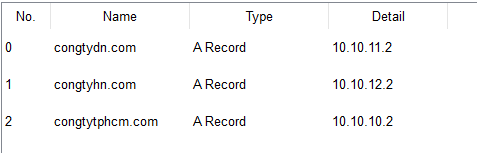
\includegraphics[width=16cm, height=4cm]{img/DNS_Service1.png}
    \caption{Đăng ký 3 tên miền cho các trụ sở}
    \label{hinh441a}
\end{figure}
\begin{figure}[H]
    \centering
    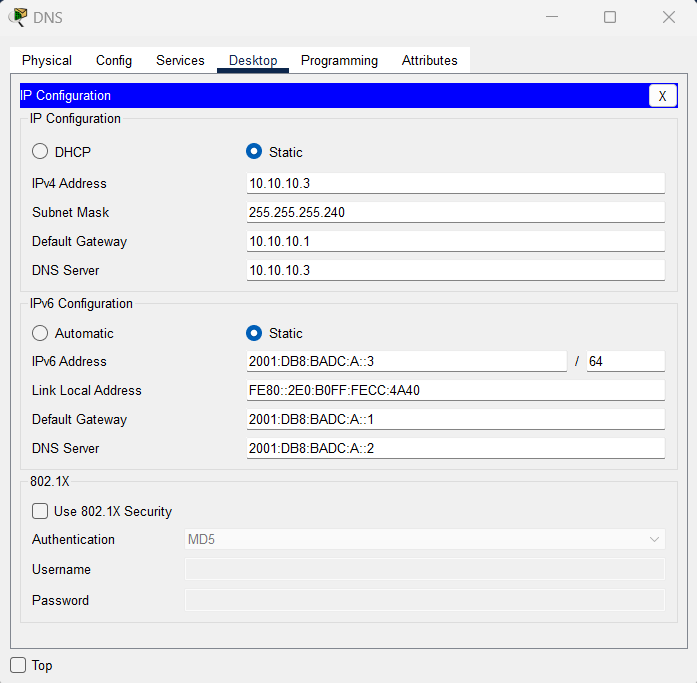
\includegraphics[width=17cm, height=14cm]{img/DNS_Service2.png}
    \caption{Cấu hình địa chỉ Ipv4 và Ipv6 cho DNS Server}
    \label{hinh441b}
\end{figure}
\subsubsection{WEB Server }
\begin{figure}[H]
    \centering
    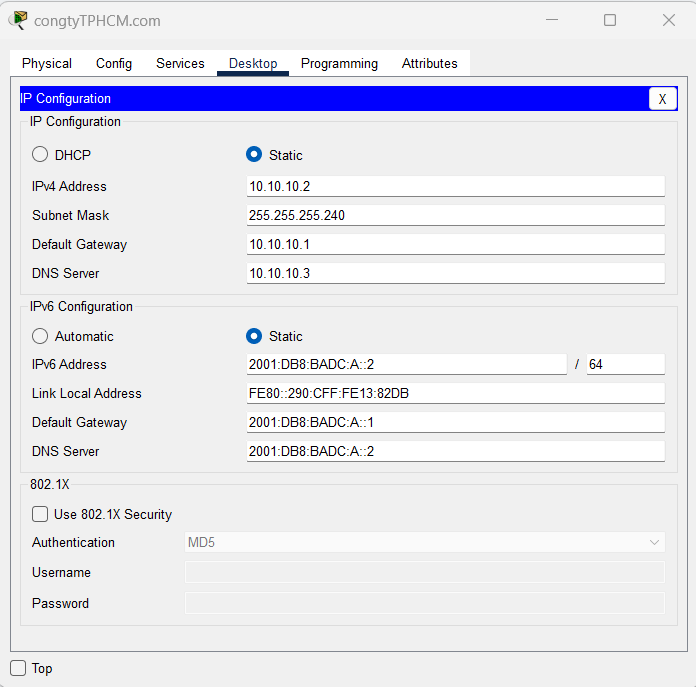
\includegraphics[width=16cm, height=14cm]{img/Web_Server1.png}
    \caption{Cấu hình địa chỉ Ipv4 và Ipv6 cho Web Server trụ sở TPHCM}
    \label{hinh421}
    
\end{figure}


\begin{figure}[H]
    \centering
    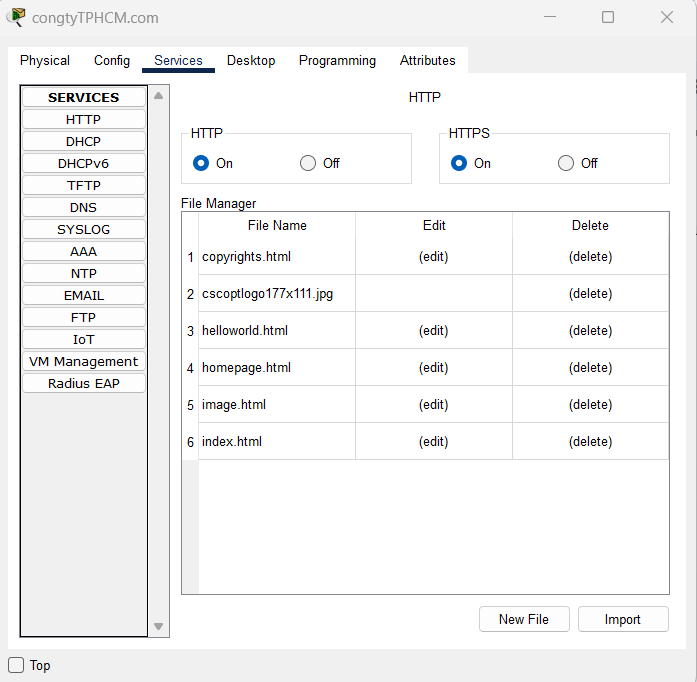
\includegraphics[width=17cm, height=12cm]{img/Web_Server2.png}
    \caption{ Bật dịch vụ HTTP}
    \label{hinh421b}
\end{figure}

\subsubsection{Mail Server}
\begin{figure}[H]
    \centering
    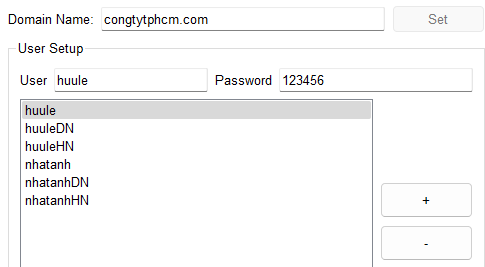
\includegraphics[width=16cm, height=6cm]{img/Mail_Server1.png}
    \caption{Bật dịch vụ Mail Server}
    \label{hinh422a}
\end{figure}
\begin{figure}[H]
    \centering
    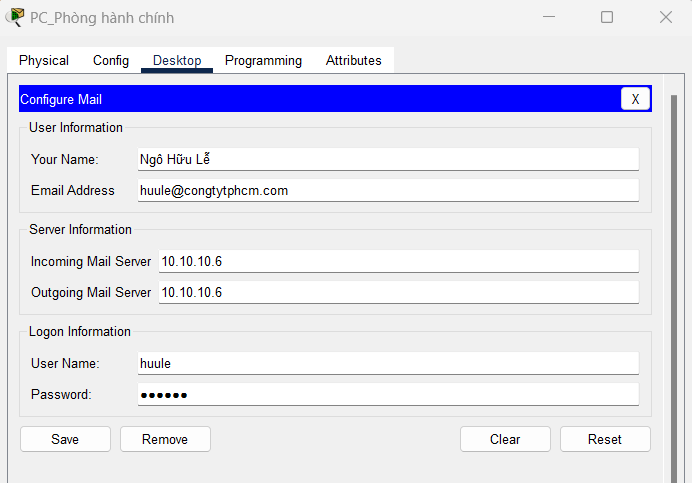
\includegraphics[width=16cm, height=10cm]{img/Mail_Server2.png}
    \caption{Cấu hình email cho máy phòng Hành chính.}
    \label{hinh422b}
\end{figure}
\begin{figure}[H]
    \centering
    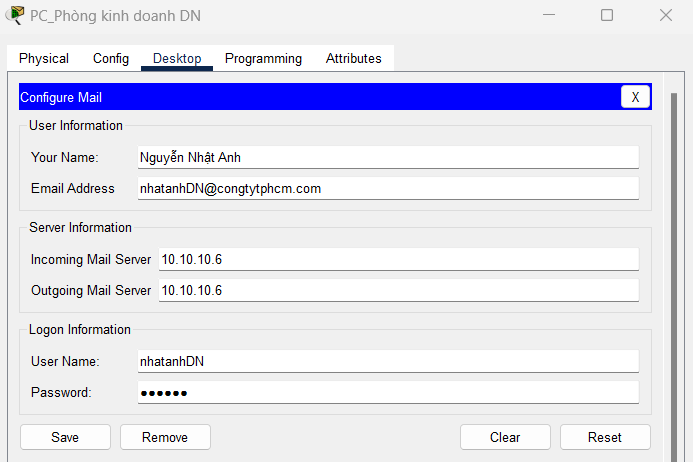
\includegraphics[width=16cm, height=10cm]{img/Mail_Server3.png}
    \caption{Cấu hình email cho máy phòng Kinh doanh chi nhánh Đà Nẵng}
    \label{hinh422c}
\end{figure}



\subsubsection{FTP Server}
\begin{figure}[H]
    \centering
    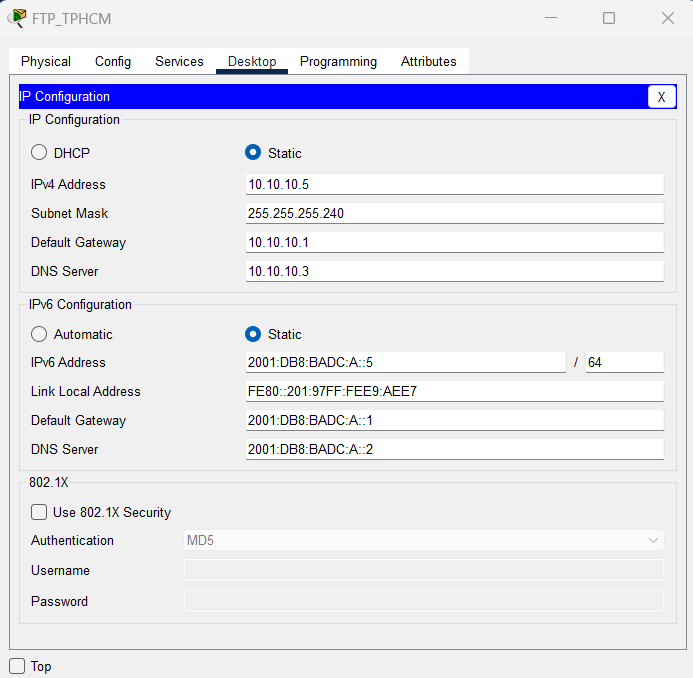
\includegraphics[width=16cm, height=14cm]{img/FTP_Server1.png}
    \caption{Cấu hình Ipv4 và Ipv6 cho FTP Server}
    \label{hinh423a}
\end{figure}

\begin{figure}[H]
    \centering
    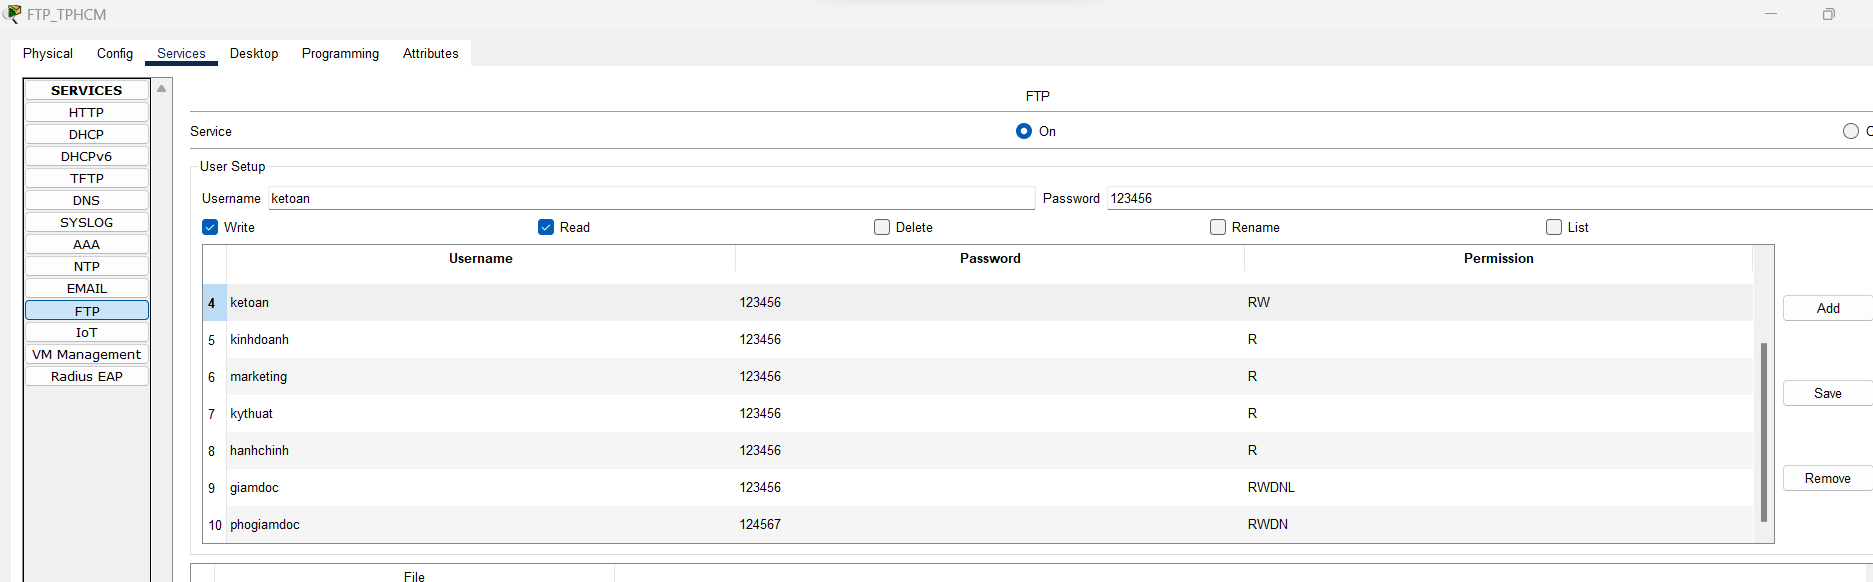
\includegraphics[width=16cm, height=8cm]{img/FTP_Server2.png}
    \caption{ Bật dịch vụ FTP và tạo tài khoản cho các phòng chức năng}
    \label{hinh423b}
\end{figure}
\subsubsection{RADIUS Server}
\begin{figure}[H]
    \centering
    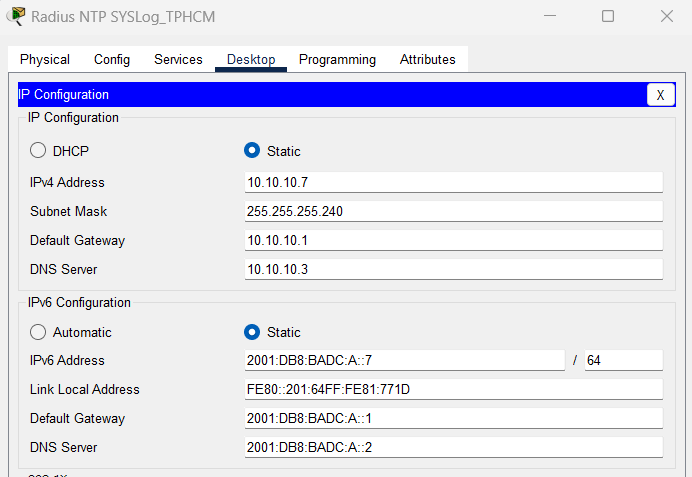
\includegraphics[width=16cm, height=14cm]{img/Radius1.png}
    \caption{Cấu hình Ipv4 và Ipv6 trên Server TPHCM.}
    \label{hinh425a}
\end{figure}

\subsubsection{NTP Server}
\begin{figure}[H]
    \centering
    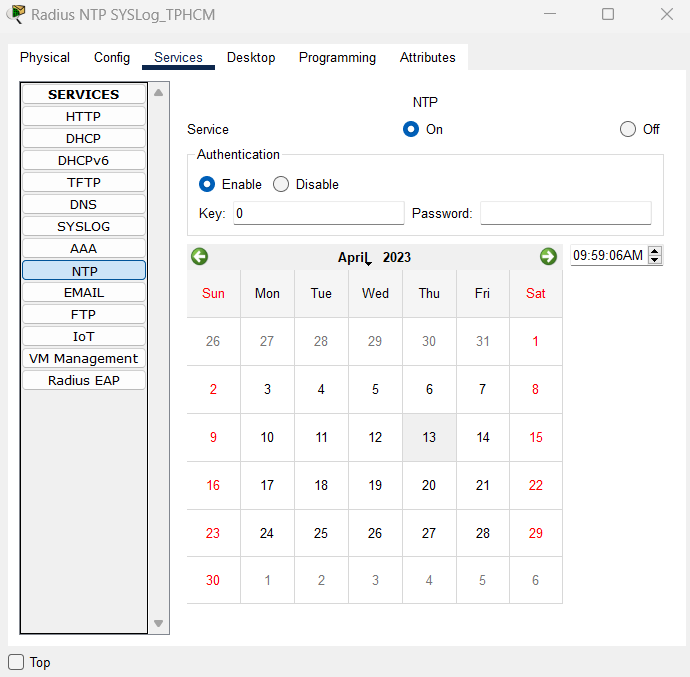
\includegraphics[width=16cm, height=14cm]{img/NTP1.png}
    \caption{ Khởi động và cài đặt dịch vụ NTP.}
    \label{hinh426}
\end{figure}
\subsubsection{Syslog Server }
\begin{figure}[H]
    \centering
    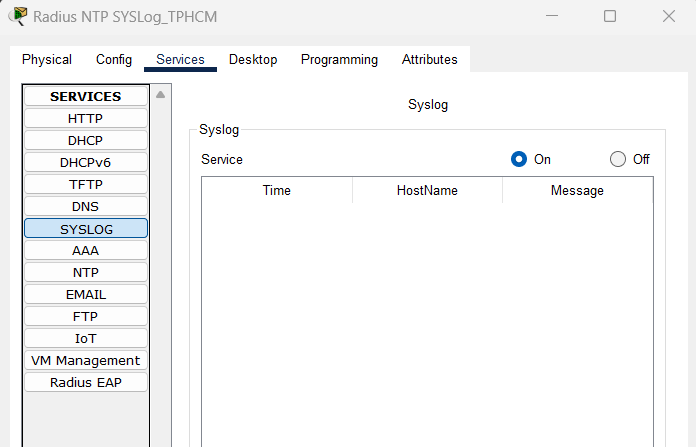
\includegraphics[width=16cm, height=6cm]{img/syslog1.png}
    \caption{ Khởi động dịch vụ Syslog}
    \label{hinh427}
\end{figure}

x\subsection{Cấu hình VLAN VÀ VTP}
\subsubsection{Khu vực TPHCM}
\hspace*{1cm}Chúng ta sẽ cấu hình các VLAN trên các Switch Layer 3, ở trụ sở TPHCM sẽ có tổng cộng 10 VLAN, bao gồm: VLAN 10 cho phòng Tiếp tân, 11 cho phòng Nhân sự, 12 cho phòng Kế toán, 13 cho phòng Kinh doanh, 14 cho phòng Marketing, 15 cho phòng Kỹ thuật, 16 cho phòng Hành chính, 17 cho phòng Giám đốc, 18 cho phòng Phó giám đốc và 100 cho Khách hàng.\\
\hspace*{1cm}Tạo VLAN Database trên Switch Distribute 1 và 2:\\
\hspace*{2cm}\textit{vlan 10\\
\hspace*{2cm}name TIEPTAN\\
\hspace*{2cm}vlan 11\\
\hspace*{2cm}name NHANSU\\
\hspace*{2cm}vlan 12\\
\hspace*{2cm}name KETOAN\\
\hspace*{2cm}vlan 13\\
\hspace*{2cm}name KINHDOANH \\
\hspace*{2cm}vlan 14\\
\hspace*{2cm}name MARKETING\\
\hspace*{2cm}vlan 15\\
\hspace*{2cm}name KYTHUAT\\
\hspace*{2cm}vlan 16\\
\hspace*{2cm}name HANHCHINH \\
\hspace*{2cm}vlan 17\\
\hspace*{2cm}name GIAMDOC\\
\hspace*{2cm}vlan 18\\
\hspace*{2cm}name PHOGIAMDOC \\
\hspace*{2cm}vlan 100\\
\hspace*{2cm}name KHACHHANG\\
\hspace*{2cm}vlan 110\\
\hspace*{2cm}name WLC\_TPHCM\\}
\hspace*{1cm}Sau khi tạo các VLAN Database, ta sẽ cấu hình giao thức VTP cho các Switch, trong đó, Switch Distribute 1 sẽ là mode Server, Distribute 2 ở mode transparent. Switch Distribute 1 ở mode server sẽ dùng để tạo bản tin VTP, lắng nghe bản tin, thêm  xóa sửa VLAN. Switch Distribute 2 sẽ ở mode transparent để backup, dùng để thêm xóa sửa VLAN nhưng chỉ có tác dụng nội bộ trên switch cấu hình Transparent.

%\renewcommand{\labelitemi}{$\blacksquare$}
%\renewcommand\labelitemii{$\nabla$}
%\renewcommand\labelitemiii{$\square$}
\begin{itemize}
  \item \textbf{Switch Distribution}
    \begin{itemize}
    \item Switch Distribute 1
    \begin{itemize}
      \item \textit{vtp domain congtytphcm.com\\
vtp version 2\\
vtp mode server\\
vtp pass congtytphcm}
    \end{itemize}
    \item Switch Distribute 2
     \begin{itemize}
      \item \textit{vtp domain congtytphcm.com\\
vtp version 2\\
vtp mode transparent\\
vtp pass congtytphcm\\}  
    \end{itemize}
    \hspace*{0.25cm} Trunking các đường  Switch Distribute 1 và 2 nối với các Switch Access 
     \item Switch Distribute 1 và 2
     \begin{itemize}
      \item \textit{interface range G1/0/1-7\\
                    switchport mode trunk}   
    \end{itemize}
   \end{itemize}
  \item \textbf{Switch Access}\\
\hspace*{1cm} Ở các Switch Access, nó sẽ ở mode client, có nhiệm vụ tạo và lắng nghe bản tin VTP\\
\hspace*{2cm}\textit{vtp domain congtytphcm.com\\
\hspace*{2cm}vtp version 2\\
\hspace*{2cm}vtp mode client\\
\hspace*{2cm}vtp pass congtytphcm\\} 
\hspace*{1cm}Các Switch Access nối với Switch Distribute 1 và 2 bằng các cổng Gigabit Ethernet 0/1 và 0/2, cho nên ta sẽ trunking các đường này.\\
\hspace*{2cm}\textit{interface range G0/1-2\\
\hspace*{2cm}switchport mode trunk\\}
\hspace*{1cm}Đối với các port nối với các PC, ta sẽ gán port acces cho từng VLAN đã định sẵn.
  \begin{itemize}
    \item \textbf{Switch Access Tiếp Tân}
    \begin{itemize}
      \item \textit{interface Fa0/1\\
switchport mode access\\
switchport access vlan 10 \\
interface Fa0/2\\
switchport mode trunk\\
switchport trunk native vlan 110\\}   
      
    \end{itemize}
    \item \textbf{Switch Access Phòng Nhân Sự}
     \begin{itemize}
      \item \textit{interface Fa0/1\\
switchport mode access\\
switchport access vlan 11\\
interface Fa0/2\\
switchport mode trunk\\
switchport trunk native vlan 110\\}
     
    \end{itemize}
     \item \textbf{Switch Access Phòng Kế Toán}
     \begin{itemize}
      \item \textit{interface Fa0/1\\
switchport mode access\\
switchport access vlan 12\\
interface Fa0/2\\
switchport mode trunk\\
switchport trunk native vlan 110\\}
     
    \end{itemize}
     \item \textbf{Switch Access Phòng Kinh Doanh}
     \begin{itemize}
      \item \textit{interface Fa0/1\\
switchport mode access\\
switchport access vlan 13\\
interface Fa0/2\\
switchport mode trunk\\
switchport trunk native vlan 110\\}
     
    \end{itemize}
     \item \textbf{Switch Access Phòng Marketing}
     \begin{itemize}
      \item \textit{interface Fa0/1\\
switchport mode access\\
switchport access vlan 14\\
interface Fa0/2\\
switchport mode trunk\\
switchport trunk native vlan 110\\}
     
    \end{itemize}
     \item \textbf{Switch Access Phòng Kỹ thuật}
     \begin{itemize}
      \item \textit{interface Fa0/1\\
switchport mode access\\
switchport access vlan 15\\
interface Fa0/2\\
switchport mode trunk\\
switchport trunk native vlan 110\\
interface Fa0/3\\
switchport mode trunk\\
switchport trunk native vlan 110\\
interface Fa0/4\\
switchport mode access\\
switchport access vlan 15\\}
     
    \end{itemize}
     \item \textbf{Switch Access Phòng Ban}
     \begin{itemize}
      \item \textit{interface Fa0/1\\
switchport mode access\\
switchport access vlan 17\\
interface Fa0/2\\
switchport mode access\\
switchport access vlan 18\\
interface Fa0/3\\
switchport mode access\\
switchport access vlan 16\\
interface Fa0/4\\
switchport mode trunk\\
switchport trunk native vlan 110\\}
     
    \end{itemize}
   \end{itemize}
\end{itemize}
\subsubsection{Khu vực Đà Nẵng}
\hspace*{1cm}Chúng ta sẽ cấu hình các VLAN trên các Switch Layer 3, ở chi nhánh Đà Nẵng sẽ có tổng cộng 6 VLAN, bao gồm : VLAN 19 cho phòng Tiếp Tân, 20 cho phòng Hành chính, VLAN 21 cho phòng Kinh doanh, VLAN 22 cho phòng Kỹ thuật, VLAN 111 cho WLC quản lý và 150 cho Khách hàng.\\
\hspace*{1cm}Tạo VLAN Database trên Switch Distribute 1 và 2:\\
\hspace*{2cm}\textit{vlan 19\\
\hspace*{2cm}name TIEPTAN\_DN \\
\hspace*{2cm}vlan 20\\
\hspace*{2cm}name HANHCHINH\_DN\\
\hspace*{2cm}vlan 21\\
\hspace*{2cm}name KINHDOANH\_DN\\
\hspace*{2cm}vlan 22\\
\hspace*{2cm}name KYTHUAT\_DN \\
\hspace*{2cm}vlan 111\\
\hspace*{2cm}name WLC\_DN \\
\hspace*{2cm}vlan 150\\
\hspace*{2cm}name KHACHHANG\_DN\\}
\hspace*{1cm}Sau khi tạo các VLAN Database, ta sẽ cấu hình giao thức VTP cho các Switch, tương tự như khu vực TPHCM.
%\renewcommand{\labelitemi}{$\blacksquare$}
%\renewcommand\labelitemii{$\nabla$}
%\renewcommand\labelitemiii{$\square$}
\begin{itemize}
  \item \textbf{Switch Distribution}
    \begin{itemize}
    \item Switch Distribute 1
    \begin{itemize}
      \item \textit{vtp domain congtydn.com \\
vtp version 2\\
vtp mode server\\
vtp pass congtydn\\}
    \end{itemize}
    \item Switch Distribute 2
     \begin{itemize}
      \item \textit{vtp domain congtydn.com\\
vtp version 2\\
vtp mode transparent\\
vtp pass congtydn\\
}  
    \end{itemize}
    \hspace*{1cm} Trunking các đường  Switch Distribute 1 và 2 nối với các Switch Access  \\
     \item Switch Distribute 1 và 2
     \begin{itemize}
      \item \textit{interface range G1/0/1-4\\
                    switchport mode trunk}   
    \end{itemize}
   \end{itemize}
  \item \textbf{Switch Access}\\
\hspace*{1cm} Ở các Switch Access, nó sẽ ở mode client, có nhiệm vụ tạo và lắng nghe bản tin VTP\\
\hspace*{2cm}\textit{vtp domain congtydn.com \\
\hspace*{2cm}vtp version 2\\
\hspace*{2cm}vtp mode client\\
\hspace*{2cm}vtp pass congtydn\\} 
\hspace*{1cm}Các Switch Access nối với Switch Distribute 1 và 2 bằng các cổng Gigabit Ethernet 0/1 và 0/2, cho nên ta sẽ trunking các đường này.\\
\hspace*{2cm}\textit{interface range G0/1-2\\
\hspace*{2cm}switchport mode trunk\\}
\hspace*{1cm}Đối với các port nối với các PC, ta sẽ gán port acces cho từng VLAN đã định sẵn.
  \begin{itemize}
    \item \textbf{Switch Access Phòng Tiếp Tân}
    \begin{itemize}
      \item \textit{interface Fa0/1\\
switchport mode access\\
switchport access vlan 19 \\
interface Fa0/2\\
switchport mode trunk\\
switchport trunk native vlan 111\\}   
      
    \end{itemize}
   
     \item \textbf{Switch Access Phòng Hành Chính}
     \begin{itemize}
      \item \textit{interface Fa0/1\\
switchport mode access\\
switchport access vlan 20\\
interface Fa0/2\\
switchport mode trunk\\
switchport trunk native vlan 111\\}
     
    \end{itemize}
     \item \textbf{witch Access Phòng Kinh Doanh}
     \begin{itemize}
      \item \textit{interface Fa0/1\\
switchport mode access\\
switchport access vlan 21\\
interface Fa0/2\\
switchport mode trunk\\
switchport trunk native vlan 111\\}
     
    \end{itemize}
     \item \textbf{Switch Access Phòng Kỹ thuật}
     \begin{itemize}
      \item \textit{interface Fa0/1\\
switchport mode access\\
switchport access vlan 22\\
interface Fa0/2\\
switchport mode access\\
switchport access vlan 22\\
interface Fa0/3\\
switchport mode trunk\\
switchport trunk native vlan 111\\
interface Fa0/4\\
switchport mode trunk\\
switchport trunk native vlan 111\\}
     
    \end{itemize}

   \end{itemize}
\end{itemize}
\subsubsection{Khu vực Hà Nội}
\hspace*{1cm}Chúng ta sẽ cấu hình các VLAN trên các Switch Layer 3, ở chi nhánh Hà Nội sẽ có tổng cộng 6 VLAN, bao gồm : VLAN 23 cho phòng Tiếp Tân, 24 cho phòng Hành chính, VLAN 25 cho phòng Kinh doanh, VLAN 26 cho phòng Kỹ thuật, VLAN 112 cho WLC quản lý và 200 cho Khách hàng.\\
\hspace*{1cm}Tạo VLAN Database trên Switch Distribute 1 và 2:\\
\hspace*{2cm}\textit{vlan 23\\
\hspace*{2cm}name TIEPTAN\_HN \\
\hspace*{2cm}vlan 24\\
\hspace*{2cm}name HANHCHINH\_HN\\
\hspace*{2cm}vlan 25\\
\hspace*{2cm}name KINHDOANH\_HN\\
\hspace*{2cm}vlan 26\\
\hspace*{2cm}name KYTHUAT\_HN \\
\hspace*{2cm}vlan 112\\
\hspace*{2cm}name WLC\_HN \\
\hspace*{2cm}vlan 200\\
\hspace*{2cm}name KHACHHANG\_HN\\}
\hspace*{1cm}Sau khi tạo các VLAN Database, ta sẽ cấu hình giao thức VTP cho các Switch, tương tự như khu vực TPHCM.
%\renewcommand{\labelitemi}{$\blacksquare$}
%\renewcommand\labelitemii{$\nabla$}
%\renewcommand\labelitemiii{$\square$}
\begin{itemize}
  \item \textbf{Switch Distribution}
    \begin{itemize}
    \item Switch Distribute 1
    \begin{itemize}
      \item \textit{vtp domain congtyhn.com \\
vtp version 2\\
vtp mode server\\
vtp pass congtyhn\\}
    \end{itemize}
    \item Switch Distribute 2
     \begin{itemize}
      \item \textit{vtp domain congtyhn.com\\
vtp version 2\\
vtp mode transparent\\
vtp pass congtyhn\\}  
    \end{itemize}
    \hspace*{1cm} Trunking các đường  Switch Distribute 1 và 2 nối với các Switch Access  \\
     \item Switch Distribute 1 và 2
     \begin{itemize}
      \item \textit{interface range G1/0/1-4\\
                    switchport mode trunk}   
    \end{itemize}
   \end{itemize}
  \item \textbf{Switch Access}\\
\hspace*{1cm} Ở các Switch Access, nó sẽ ở mode client, có nhiệm vụ tạo và lắng nghe bản tin VTP\\
\hspace*{2cm}\textit{vtp domain congtyhn.com \\
\hspace*{2cm}vtp version 2\\
\hspace*{2cm}vtp mode client\\
\hspace*{2cm}vtp pass congtyhn\\} 
\hspace*{1cm}Các Switch Access nối với Switch Distribute 1 và 2 bằng các cổng Gigabit Ethernet 0/1 và 0/2, cho nên ta sẽ trunking các đường này.\\
\hspace*{2cm}\textit{interface range G0/1-2\\
\hspace*{2cm}switchport mode trunk\\}
\hspace*{1cm}Đối với các port nối với các PC, ta sẽ gán port acces cho từng VLAN đã định sẵn.
  \begin{itemize}
    \item \textbf{Switch Access Phòng Tiếp Tân}
    \begin{itemize}
      \item \textit{interface Fa0/1\\
\hspace*{2cm}switchport mode access\\
\hspace*{2cm}switchport access vlan 23 \\
\hspace*{2cm}interface Fa0/2\\
\hspace*{2cm}switchport mode trunk\\
\hspace*{2cm}switchport trunk native vlan 112\\}   
      
    \end{itemize}
   
     \item \textbf{Switch Access Phòng Hành Chính}
     \begin{itemize}
      \item \textit{interface Fa0/1\\
\hspace*{2cm}switchport mode access\\
\hspace*{2cm}switchport access vlan 24\\
\hspace*{2cm}interface Fa0/2\\
\hspace*{2cm}switchport mode trunk\\
\hspace*{2cm}switchport trunk native vlan 112\\}
     
    \end{itemize}
     \item \textbf{witch Access Phòng Kinh Doanh}
     \begin{itemize}
      \item \textit{interface Fa0/1\\
\hspace*{2cm}switchport mode access\\
\hspace*{2cm}switchport access vlan 25\\
\hspace*{2cm}interface Fa0/2\\
\hspace*{2cm}switchport mode trunk\\
\hspace*{2cm}switchport trunk native vlan 112\\}
     
    \end{itemize}
     \item \textbf{Switch Access Phòng Kỹ thuật}
     \begin{itemize}
      \item \textit{interface Fa0/1\\
\hspace*{2cm}switchport mode access\\
\hspace*{2cm}switchport access vlan 26\\
\hspace*{2cm}interface Fa0/2\\
\hspace*{2cm}switchport mode access\\
\hspace*{2cm}switchport access vlan 26\\
\hspace*{2cm}interface Fa0/3\\
\hspace*{2cm}switchport mode trunk\\
\hspace*{2cm}switchport trunk native vlan 112\\
\hspace*{2cm}interface Fa0/4\\
\hspace*{2cm}switchport mode trunk\\
\hspace*{2cm}switchport trunk native vlan 112\\}
     
    \end{itemize}

   \end{itemize}
\end{itemize}
\subsection{Cấu hình WLC và Light Weight Access Point }
\begin{figure}[H]
    \centering
    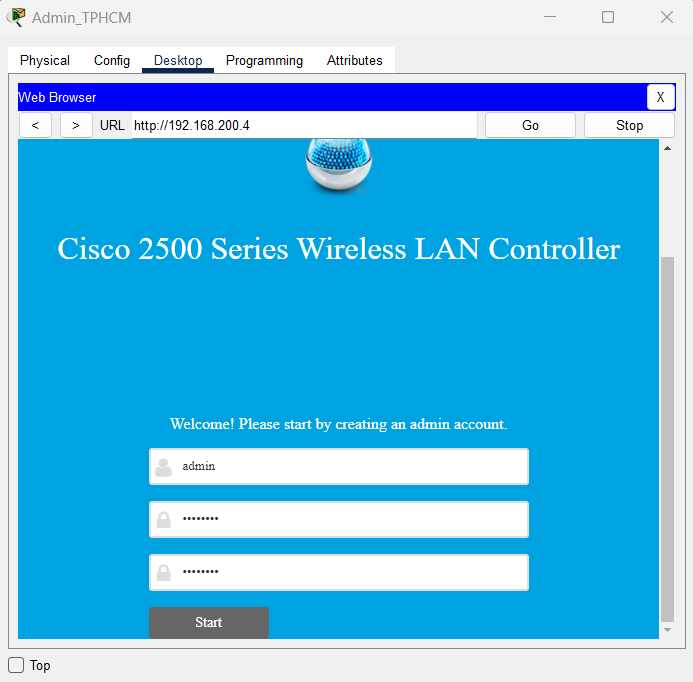
\includegraphics[width=12cm, height=6cm]{img/WLC1.png}
    \caption{Tạo tài khoản }
    \label{hinh46a}
\end{figure}
\hspace*{1cm}Truy cập vào địa chỉ IP đã đặt trên WLC để tạo tài khoản đăng nhập, sau đó tiến hành tạo các Interface và WLAN phù hợp. Sau khi tạo xong, chọn apply để tạo.\\
\begin{figure}[H]
    \centering
    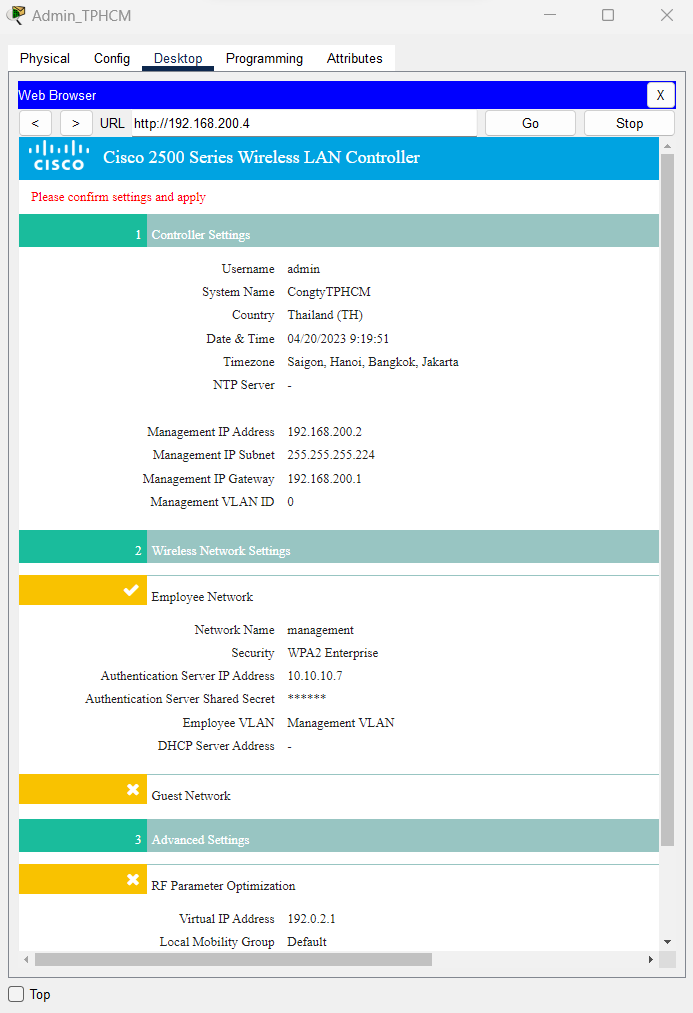
\includegraphics[width=16cm, height=18cm]{img/WLC2.png}
    \caption{Thông tin sau khi tạo}
    \label{hinh45b}
\end{figure}
    
\hspace*{1cm}Sau khi tạo tài khoản, truy cập địa chỉ: https://192.168.200.2 để đăng nhập vào giao diện WLC. Đăng nhập với tài khoản admin và mật khẩu Cisco123. Sau khi hiển thị giao diện WLC, nhóm em sẽ tiến hành tạo các Interface và các WLAN ID.\\
\begin{figure}[H]
    \centering
    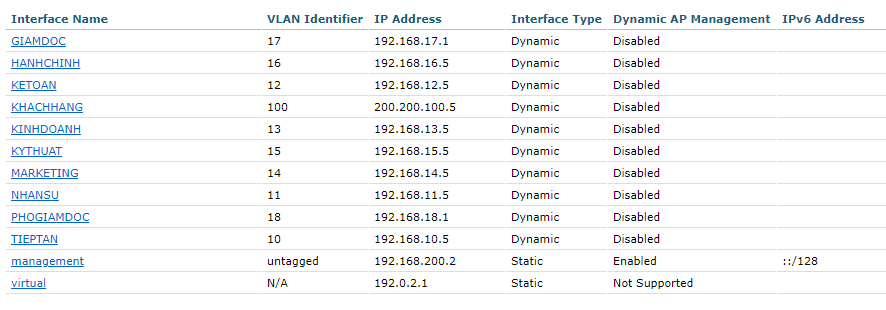
\includegraphics[width=16cm, height=14cm]{img/interfaceWLAN.png}
    \caption{Tạo Interface cho các WLAN}
    \label{hinh46c}
\end{figure}

\begin{figure}[H]
    \centering
    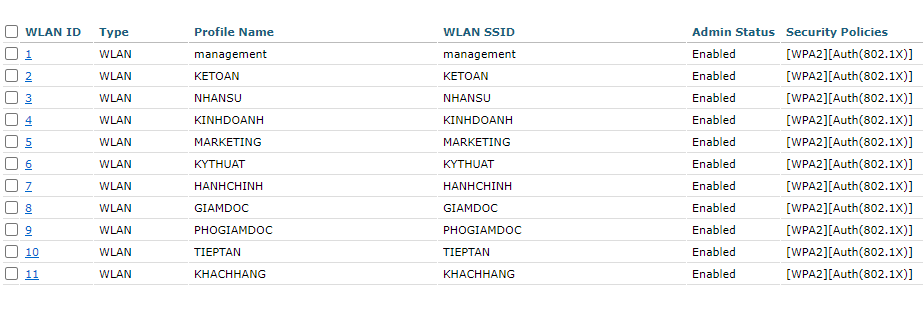
\includegraphics[width=16cm, height=10cm]{img/IDWLAN.png}
    \caption{Tạo WLAN ID }
    \label{hinh46d}
\end{figure}
\hspace*{1cm}Tạo WLAN, ở Layer 2 Security , chọn WPA +WPA2 với thông số mã hóa WPA2 là AES và khóa xác thực là 802.1X. Sau đó, ở phần cấu hình AAA, chọn Server Radius với số port khớp với Server mà chúng ta đã tạo ở hệ thống.\\
\begin{figure}[H]
    \centering
    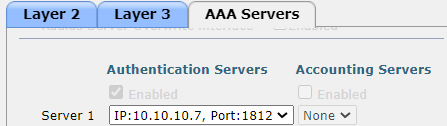
\includegraphics[width=12cm, height=6cm]{img/4.6e.png}
    \caption{Chọn dải IP Radius phù hợp}
    \label{hinh46e}
\end{figure}
\hspace*{1cm}Ở phần Flex Connect, chúng ta sẽ chọn hai thông số là Flex Connect Switching và Local Auth để tạo đường hầm CAPWAP đến WLC, một là để quản lý, còn lại là lưu lượng dữ liệu.\\
\hspace*{1cm}Sau khi đã tạo các WLAN và các Light Access Point đã kết nối được, lúc này chúng ta sẽ chia các Light Access Point ở các tầng để phát cố định các Wifi cần thiết. Ở tầng 1, chúng ta sẽ cho LAP chỉ phát một wifi cho phòng lễ tân, còn ở tầng 2, LAP sẽ phát wifi cho ba phòng hành chính, phó giám đốc và giám đốc, 3 tầng còn lại mỗi LAP sẽ phát wifi cho các phòng chức năng tương ứng.\\
\begin{figure}[H]
    \centering
    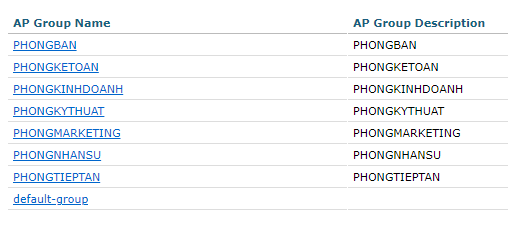
\includegraphics[width=16cm, height=6cm]{img/APGroup.png}
    \caption{Tạo AP Group}
    \label{hinh46f}
\end{figure}
\begin{figure}[H]
    \centering
    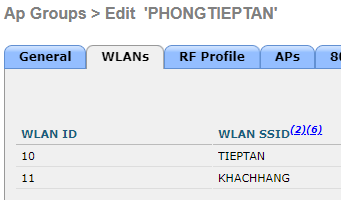
\includegraphics[width=16cm, height=10cm]{img/phongtieptan.png}
    \caption{Cấu hình các LAP phát Wifi cho WLAN}
    \label{hinh46h}
\end{figure}
\hspace*{0.25cm} Sau khi đã cấu hình xong , vào các PC tạo profile để kết nối.
\hspace*{0.25cm}Cấu hình tương tự ở chi nhánh Đà Nẵng và Hà Nội.

\subsection{Cấu hình DHCPv4 và DHCPv6}
\subsubsection{Khu vực TPHCM}
\hspace*{0.25cm}Tạo các pool DHCP cho các VLAN, bao gồm ipv4 và ipv6. Cấu hình của chức năng này sẽ được cấu hình trên DHCP server, cấp phát các IP động xuống cho các VLAN.\\
\begin{figure}[H]
    \centering
    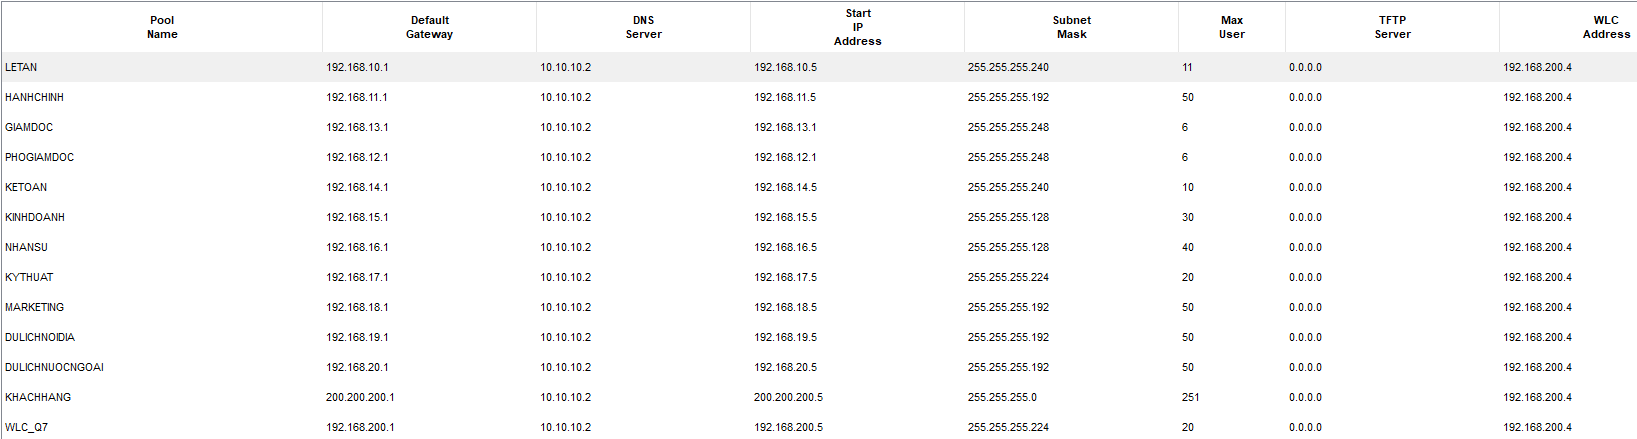
\includegraphics[width=16cm, height=8cm]{img/471.png}
    \caption{Tạo các Pool DHCP trên Server}
    \label{hinh471}
\end{figure}
\hspace*{0.25cm}Sau khi tạo pool trên Server, cấu hình inter-vlan trên hai switch Distribution như sau\\
\hspace*{1cm}\textbf{Switch Distribution 1}\\
\hspace*{2cm}\textit{int vlan 10\\
\hspace*{2cm}ip add 192.168.10.3 255.255.255.240\\
\hspace*{2cm}ipv6 add 2001:db8:acad:a::3/64\\
\hspace*{2cm}ip help 10.10.10.4\\
\hspace*{2cm}int vlan 11\\
\hspace*{2cm}ip add 192.168.11.3 255.255.255.128\\
\hspace*{2cm}ipv6 add 2001:db8:acad:b::3/64\\
\hspace*{2cm}ip help 10.10.10.4\\
\hspace*{2cm}int vlan 12\\
\hspace*{2cm}ip add 192.168.12.3 255.255.255.240\\
\hspace*{2cm}ipv6 add 2001:db8:acad:c::3/64\\
\hspace*{2cm}ip help 10.10.10.4\\
\hspace*{2cm}int vlan 13\\
\hspace*{2cm}ip add 192.168.13.3 255.255.255.192\\
\hspace*{2cm}ipv6 add 2001:db8:acad:d::3/64\\
\hspace*{2cm}ip help 10.10.10.4\\
\hspace*{2cm}int vlan 14\\
\hspace*{2cm}ip add 192.168.14.3 255.255.255.192\\
\hspace*{2cm}ipv6 add 2001:db8:acad:e::3/64\\
\hspace*{2cm}ip help 10.10.10.4\\
\hspace*{2cm}int vlan 15\\
\hspace*{2cm}ip add 192.168.15.3 255.255.255.224\\
\hspace*{2cm}ipv6 add 2001:db8:acad:f::3/64\\
\hspace*{2cm}ip help 10.10.10.4\\
\hspace*{2cm}int vlan 16\\
\hspace*{2cm}ip add 192.168.16.3 255.255.255.192\\
\hspace*{2cm}ipv6 add 2001:db8:acad:16::3/64 \\
\hspace*{2cm}ip help 10.10.10.4\\
\hspace*{2cm}int vlan 17\\
\hspace*{2cm}ip add 192.168.17.3 255.255.255.240\\
\hspace*{2cm}ipv6 add 2001:db8:acad:17::3/64 \\
\hspace*{2cm}ip help 10.10.10.4\\
\hspace*{2cm}int vlan 18\\
\hspace*{2cm}ip add 192.168.18.3 255.255.255.240\\
\hspace*{2cm}ipv6 add 2001:db8:acad:18::3/64 \\
\hspace*{2cm}ip help 10.10.10.4\\
\hspace*{2cm}int vlan 100\\
\hspace*{2cm}ip add 200.200.100.3 255.255.255.0 \\
\hspace*{2cm}ipv6 add 2001:db8:acad:100::3/64 \\
\hspace*{2cm}ip help 10.10.10.4\\
\hspace*{2cm}int vlan 110\\
\hspace*{2cm}ip add 192.168.200.3 255.255.255.224 \\
\hspace*{2cm}ipv6 add 2001:db8:acad:110::3/64 \\
\hspace*{2cm}ip help 10.10.10.4\\
}

\hspace*{1cm}\textbf{Switch Distribution 2}\\
\hspace*{2cm}\textit{int vlan 10\\
\hspace*{2cm}ip add 192.168.10.2 255.255.255.240\\
\hspace*{2cm}ipv6 add 2001:db8:acad:a::2/64\\
\hspace*{2cm}ip help 10.10.10.4\\
\hspace*{2cm}int vlan 11\\
\hspace*{2cm}ip add 192.168.11.2 255.255.255.128\\
\hspace*{2cm}ipv6 add 2001:db8:acad:b::2/64\\
\hspace*{2cm}ip help 10.10.10.4\\
\hspace*{2cm}int vlan 12\\
\hspace*{2cm}ip add 192.168.12.2 255.255.255.240\\
\hspace*{2cm}ipv6 add 2001:db8:acad:c::2/64\\
\hspace*{2cm}ip help 10.10.10.4\\
\hspace*{2cm}int vlan 13\\
\hspace*{2cm}ip add 192.168.13.2 255.255.255.192\\
\hspace*{2cm}ipv6 add 2001:db8:acad:d::2/64\\
\hspace*{2cm}ip help 10.10.10.4\\
\hspace*{2cm}int vlan 14\\
\hspace*{2cm}ip add 192.168.14.2 255.255.255.192\\
\hspace*{2cm}ipv6 add 2001:db8:acad:e::2/64\\
\hspace*{2cm}ip help 10.10.10.4\\
\hspace*{2cm}int vlan 15\\
\hspace*{2cm}ip add 192.168.15.2 255.255.255.224\\
\hspace*{2cm}ipv6 add 2001:db8:acad:f::2/64\\
\hspace*{2cm}ip help 10.10.10.4\\
\hspace*{2cm}int vlan 16\\
\hspace*{2cm}ip add 192.168.16.2 255.255.255.192\\
\hspace*{2cm}ipv6 add 2001:db8:acad:16::2/64 \\
\hspace*{2cm}ip help 10.10.10.4\\
\hspace*{2cm}int vlan 17\\
\hspace*{2cm}ip add 192.168.17.2 255.255.255.240\\
\hspace*{2cm}ipv6 add 2001:db8:acad:17::2/64 \\
\hspace*{2cm}ip help 10.10.10.4\\
\hspace*{2cm}int vlan 18\\
\hspace*{2cm}ip add 192.168.18.2 255.255.255.240\\
\hspace*{2cm}ipv6 add 2001:db8:acad:18::2/64 \\
\hspace*{2cm}ip help 10.10.10.4\\
\hspace*{2cm}int vlan 100\\
\hspace*{2cm}ip add 200.200.100.2 255.255.255.0 \\
\hspace*{2cm}ipv6 add 2001:db8:acad:100::2/64 \\
\hspace*{2cm}ip help 10.10.10.4\\
\hspace*{2cm}int vlan 110\\
\hspace*{2cm}ip add 192.168.200.2 255.255.255.224 \\
\hspace*{2cm}ipv6 add 2001:db8:acad:110::2/64 \\
\hspace*{2cm}ip help 10.10.10.4\\}
\subsubsection{Khu vực Đà Nẵng}
\hspace*{0.25cm}Tạo các pool DHCP cho các VLAN tương tự khu vực TPHCM\\
\begin{figure}[H]
    \centering
    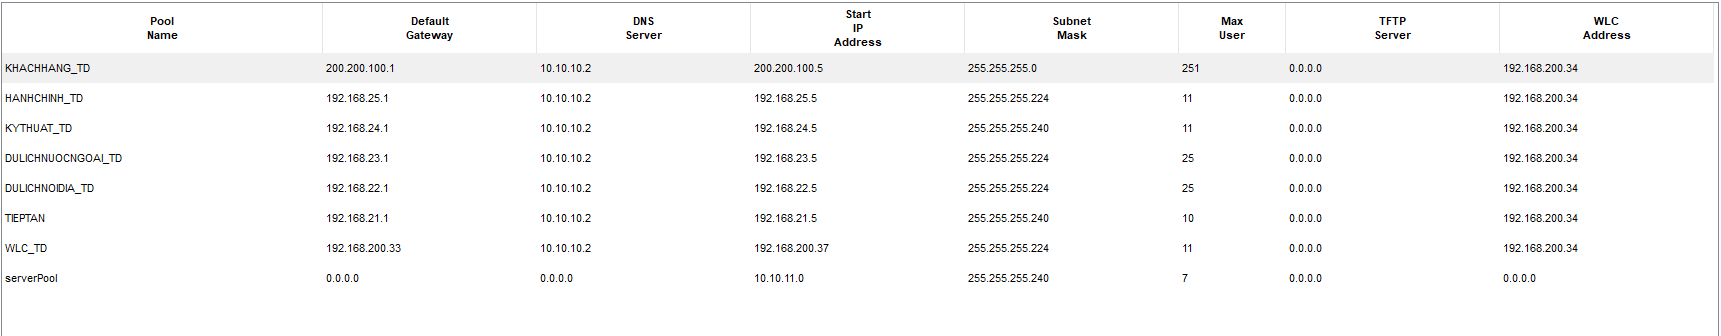
\includegraphics[width=16cm, height=8cm]{img/472.png}
    \caption{Tạo các Pool DHCP trên Server}
    \label{hinh472}
\end{figure}
\hspace*{0.25cm}Sau khi tạo pool trên Server, cấu hình inter-vlan trên hai switch Distribution như sau\\
\hspace*{1cm}\textbf{Switch Distribution 1}\\
\hspace*{2cm}\textit{int vlan 19\\
\hspace*{2cm}ip add 192.168.19.3 255.255.255.240\\
\hspace*{2cm}ipv6 add 2001:db8:acad:19::3/64\\
\hspace*{2cm}ip help 10.10.11.3\\
\hspace*{2cm}int vlan 20\\
\hspace*{2cm}ip add 192.168.20.3 255.255.255.224\\
\hspace*{2cm}ipv6 add 2001:db8:acad:20::3/64\\
\hspace*{2cm}ip help 10.10.11.3\\
\hspace*{2cm}int vlan 21\\
\hspace*{2cm}ip add 192.168.21.3 255.255.255.192\\
\hspace*{2cm}ipv6 add 2001:db8:acad:21::3/64\\
\hspace*{2cm}ip help 10.10.11.3\\
\hspace*{2cm}int vlan 22\\
\hspace*{2cm}ip add 192.168.22.3 255.255.255.240\\
\hspace*{2cm}ipv6 add 2001:db8:acad:22::3/64\\
\hspace*{2cm}ip help 10.10.11.3\\
\hspace*{2cm}int vlan 150\\
\hspace*{2cm}ip add 200.200.150.3 255.255.255.0\\
\hspace*{2cm}ipv6 add 2001:db8:acad:150::3/64\\
\hspace*{2cm}ip help 10.10.11.3\\
\hspace*{2cm}int vlan 111\\
\hspace*{2cm}ip add 192.168.200.36 255.255.255.224 \\
\hspace*{2cm}ipv6 add 2001:db8:acad:111::3/64\\
\hspace*{2cm}ip help 10.10.11.3\\}
\hspace*{1cm}\textbf{Switch Distribution 2}\\
\hspace*{2cm}\textit{int vlan 19\\
\hspace*{2cm}ip add 192.168.19.2 255.255.255.240\\
\hspace*{2cm}ipv6 add 2001:db8:acad:19::2/64\\
\hspace*{2cm}ip help 10.10.11.3\\
\hspace*{2cm}int vlan 20\\
\hspace*{2cm}ip add 192.168.20.2 255.255.255.224\\
\hspace*{2cm}ipv6 add 2001:db8:acad:20::2/64\\
\hspace*{2cm}ip help 10.10.11.3\\
\hspace*{2cm}int vlan 21\\
\hspace*{2cm}ip add 192.168.21.2 255.255.255.192\\
\hspace*{2cm}ipv6 add 2001:db8:acad:21::2/64\\
\hspace*{2cm}ip help 10.10.11.3\\
\hspace*{2cm}int vlan 22\\
\hspace*{2cm}ip add 192.168.22.2 255.255.255.240\\
\hspace*{2cm}ipv6 add 2001:db8:acad:22::2/64\\
\hspace*{2cm}ip help 10.10.11.3\\
\hspace*{2cm}int vlan 150\\
\hspace*{2cm}ip add 200.200.150.2 255.255.255.0\\
\hspace*{2cm}ipv6 add 2001:db8:acad:150::2/64\\
\hspace*{2cm}ip help 10.10.11.3\\
\hspace*{2cm}int vlan 111\\
\hspace*{2cm}ip add 192.168.200.35 255.255.255.224 \\
\hspace*{2cm}ipv6 add 2001:db8:acad:111::2/64\\
\hspace*{2cm}ip help 10.10.11.3\\}

\subsubsection{Khu vực Hà Nội}
\hspace*{0.25cm}Tạo các pool DHCP cho các VLAN tương tự khu vực TPHCM\\
\begin{figure}[H]
    \centering
    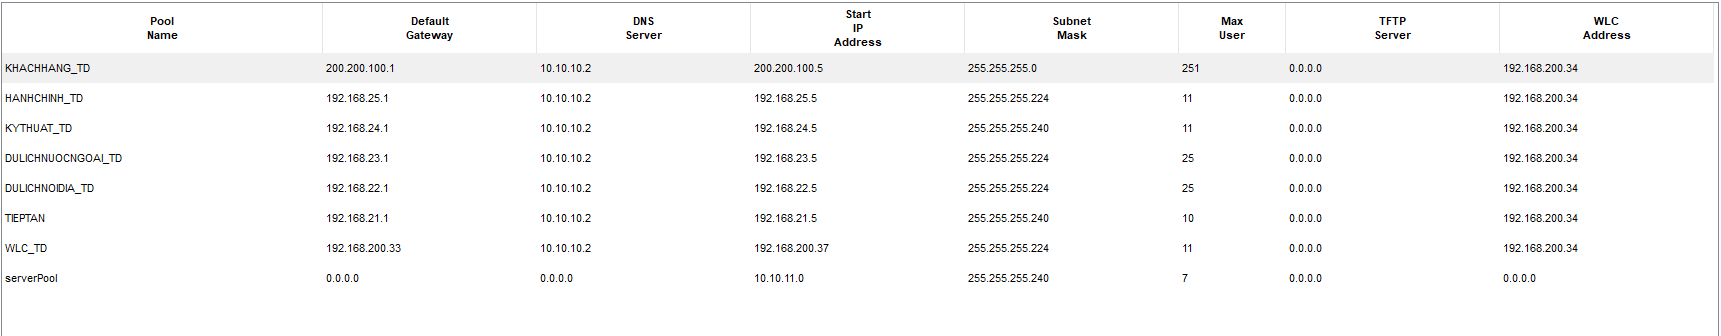
\includegraphics[width=16cm, height=8cm]{img/472.png}
    \caption{Tạo các Pool DHCP trên Server}
    \label{hinh472}
\end{figure}
\hspace*{0.25cm}Sau khi tạo pool trên Server, cấu hình inter-vlan trên hai switch Distribution như sau\\
\hspace*{1cm}\textbf{Switch Distribution 1}\\
\hspace*{2cm}\textit{int vlan 23\\
\hspace*{2cm}ip add 192.168.23.3 255.255.255.240\\
\hspace*{2cm}ipv6 add 2001:db8:acad:23::3/64\\
\hspace*{2cm}ip help 10.10.12.3\\
\hspace*{2cm}int vlan 24\\
\hspace*{2cm}ip add 192.168.24.3 255.255.255.224\\
\hspace*{2cm}ipv6 add 2001:db8:acad:24::3/64\\
\hspace*{2cm}ip help 10.10.12.3\\
\hspace*{2cm}int vlan 25\\
\hspace*{2cm}ip add 192.168.25.3 255.255.255.192\\
\hspace*{2cm}ipv6 add 2001:db8:acad:25::3/64\\
\hspace*{2cm}ip help 10.10.12.3\\
\hspace*{2cm}int vlan 26\\
\hspace*{2cm}ip add 192.168.26.3 255.255.255.240\\
\hspace*{2cm}ipv6 add 2001:db8:acad:26::3/64\\
\hspace*{2cm}ip help 10.10.12.3\\
\hspace*{2cm}int vlan 200\\
\hspace*{2cm}ip add 200.200.200.3 255.255.255.0\\
\hspace*{2cm}ipv6 add 2001:db8:acad:200::3/64\\
\hspace*{2cm}ip help 10.10.12.3\\
\hspace*{2cm}int vlan 112\\
\hspace*{2cm}ip add 192.168.200.68 255.255.255.224 \\
\hspace*{2cm}ipv6 add 2001:db8:acad:112::3/64\\
\hspace*{2cm}ip help 10.10.12.3\\}
\hspace*{1cm}\textbf{Switch Distribution 2}\\
\hspace*{2cm}\textit{int vlan 23\\
\hspace*{2cm}ip add 192.168.23.2 255.255.255.240\\
\hspace*{2cm}ipv6 add 2001:db8:acad:23::2/64\\
\hspace*{2cm}ip help 10.10.12.3\\
\hspace*{2cm}int vlan 24\\
\hspace*{2cm}ip add 192.168.24.2 255.255.255.224\\
\hspace*{2cm}ipv6 add 2001:db8:acad:24::2/64\\
\hspace*{2cm}ip help 10.10.12.3\\
\hspace*{2cm}int vlan 25\\
\hspace*{2cm}ip add 192.168.25.2 255.255.255.192\\
\hspace*{2cm}ipv6 add 2001:db8:acad:25::2/64\\
\hspace*{2cm}ip help 10.10.12.3\\
\hspace*{2cm}int vlan 26\\
\hspace*{2cm}ip add 192.168.26.2 255.255.255.240\\
\hspace*{2cm}ipv6 add 2001:db8:acad:26::2/64\\
\hspace*{2cm}ip help 10.10.12.3\\
\hspace*{2cm}int vlan 200\\
\hspace*{2cm}ip add 200.200.200.2 255.255.255.0\\
\hspace*{2cm}ipv6 add 2001:db8:acad:200::2/64\\
\hspace*{2cm}ip help 10.10.12.3\\
\hspace*{2cm}int vlan 112\\
\hspace*{2cm}ip add 192.168.200.67 255.255.255.224 \\
\hspace*{2cm}ipv6 add 2001:db8:acad:112::2/64\\
\hspace*{2cm}ip help 10.10.12.3\\}

\subsection{Cấu hình DHCP Snooping}
\subsubsection{Khu vực Quận 7}
\hspace*{0.25cm}Để chống giả mạo DHCP Server, ngăn chặn những cuộc tấn công của tin tặc vào hệ thống mạng và đánh cắp các thông tin quan trọng của doanh nghiệp, chúng ta sẽ sử dụng DHCP Snooping, khi đó máy tính sẽ được bảo vệ và ngăn chặn khỏi các cuộc tấn công này.\\
\hspace*{1cm}\textbf{Switch Access Lễ Tân}\\
\hspace*{2cm}\textit{no ip dhcp snooping information option\\
\hspace*{2cm}ip dhcp snooping vlan 10\\
\hspace*{2cm}ip dhcp snooping vlan 11\\
\hspace*{2cm}ip dhcp snooping vlan 12\\
\hspace*{2cm}ip dhcp snooping vlan 13\\
\hspace*{2cm}ip dhcp snooping vlan 14\\
\hspace*{2cm}ip dhcp snooping vlan 15\\
\hspace*{2cm}ip dhcp snooping vlan 16\\
\hspace*{2cm}ip dhcp snooping vlan 17\\
\hspace*{2cm}ip dhcp snooping vlan 18\\
\hspace*{2cm}ip dhcp snooping vlan 19\\
\hspace*{2cm}ip dhcp snooping vlan 20\\
\hspace*{2cm}ip dhcp snooping vlan 110\\
\hspace*{2cm}ip dhcp snooping vlan 200\\
\hspace*{2cm}inter range g0/1-2\\
\hspace*{2cm}ip dhcp snooping trust\\
\hspace*{2cm}ex\\
\hspace*{2cm}inter range f0/1-3\\
\hspace*{2cm}ip dhcp snooping limit rate 30\\}
\hspace*{1cm}\textbf{Switch Access Tầng 2}\\
\hspace*{2cm}\textit{no ip dhcp snooping information option\\
\hspace*{2cm}ip dhcp snooping vlan 10\\
\hspace*{2cm}ip dhcp snooping vlan 11\\
\hspace*{2cm}ip dhcp snooping vlan 12\\
\hspace*{2cm}ip dhcp snooping vlan 13\\
\hspace*{2cm}ip dhcp snooping vlan 14\\
\hspace*{2cm}ip dhcp snooping vlan 15\\
\hspace*{2cm}ip dhcp snooping vlan 16\\
\hspace*{2cm}ip dhcp snooping vlan 17\\
\hspace*{2cm}ip dhcp snooping vlan 18\\
\hspace*{2cm}ip dhcp snooping vlan 19\\
\hspace*{2cm}ip dhcp snooping vlan 20\\
\hspace*{2cm}ip dhcp snooping vlan 110\\
\hspace*{2cm}ip dhcp snooping vlan 200\\
\hspace*{2cm}inter range g0/1-2\\
\hspace*{2cm}ip dhcp snooping trust\\
\hspace*{2cm}ex\\
\hspace*{2cm}inter range f0/1-4\\
\hspace*{2cm}ip dhcp snooping limit rate 30\\}
\hspace*{1cm}\textbf{Switch Access Kế toán}\\
\hspace*{2cm}\textit{no ip dhcp snooping information option\\
\hspace*{2cm}ip dhcp snooping vlan 10\\
\hspace*{2cm}ip dhcp snooping vlan 11\\
\hspace*{2cm}ip dhcp snooping vlan 12\\
\hspace*{2cm}ip dhcp snooping vlan 13\\
\hspace*{2cm}ip dhcp snooping vlan 14\\
\hspace*{2cm}ip dhcp snooping vlan 15\\
\hspace*{2cm}ip dhcp snooping vlan 16\\
\hspace*{2cm}ip dhcp snooping vlan 17\\
\hspace*{2cm}ip dhcp snooping vlan 18\\
\hspace*{2cm}ip dhcp snooping vlan 19\\
\hspace*{2cm}ip dhcp snooping vlan 20\\
\hspace*{2cm}ip dhcp snooping vlan 110\\
\hspace*{2cm}ip dhcp snooping vlan 200\\
\hspace*{2cm}inter range g0/1-2\\
\hspace*{2cm}ip dhcp snooping trust\\
\hspace*{2cm}ex\\
\hspace*{2cm}inter range f0/1-2\\
\hspace*{2cm}ip dhcp snooping limit rate 30\\}
\hspace*{1cm}\textbf{Switch Access Kinh Doanh}\\
\hspace*{2cm}\textit{no ip dhcp snooping information option\\
\hspace*{2cm}ip dhcp snooping vlan 10\\
\hspace*{2cm}ip dhcp snooping vlan 11\\
\hspace*{2cm}ip dhcp snooping vlan 12\\
\hspace*{2cm}ip dhcp snooping vlan 13\\
\hspace*{2cm}ip dhcp snooping vlan 14\\
\hspace*{2cm}ip dhcp snooping vlan 15\\
\hspace*{2cm}ip dhcp snooping vlan 16\\
\hspace*{2cm}ip dhcp snooping vlan 17\\
\hspace*{2cm}ip dhcp snooping vlan 18\\
\hspace*{2cm}ip dhcp snooping vlan 19\\
\hspace*{2cm}ip dhcp snooping vlan 20\\
\hspace*{2cm}ip dhcp snooping vlan 110\\
\hspace*{2cm}ip dhcp snooping vlan 200\\
\hspace*{2cm}inter range g0/1-2\\
\hspace*{2cm}ip dhcp snooping trust\\
\hspace*{2cm}ex\\
\hspace*{2cm}inter range f0/1-2\\
\hspace*{2cm}ip dhcp snooping limit rate 30\\}
\hspace*{1cm}\textbf{Switch Access Nhân sự}\\
\hspace*{2cm}\textit{no ip dhcp snooping information option\\
\hspace*{2cm}ip dhcp snooping vlan 10\\
\hspace*{2cm}ip dhcp snooping vlan 11\\
\hspace*{2cm}ip dhcp snooping vlan 12\\
\hspace*{2cm}ip dhcp snooping vlan 13\\
\hspace*{2cm}ip dhcp snooping vlan 14\\
\hspace*{2cm}ip dhcp snooping vlan 15\\
\hspace*{2cm}ip dhcp snooping vlan 16\\
\hspace*{2cm}ip dhcp snooping vlan 17\\
\hspace*{2cm}ip dhcp snooping vlan 18\\
\hspace*{2cm}ip dhcp snooping vlan 19\\
\hspace*{2cm}ip dhcp snooping vlan 20\\
\hspace*{2cm}ip dhcp snooping vlan 110\\
\hspace*{2cm}ip dhcp snooping vlan 200\\
\hspace*{2cm}inter range g0/1-2\\
\hspace*{2cm}ip dhcp snooping trust\\
\hspace*{2cm}ex\\
\hspace*{2cm}inter range f0/1-2\\
\hspace*{2cm}ip dhcp snooping limit rate 30\\}
\hspace*{1cm}\textbf{Switch Access Kỹ Thuật}\\
\hspace*{2cm}\textit{no ip dhcp snooping information option\\
\hspace*{2cm}ip dhcp snooping vlan 10\\
\hspace*{2cm}ip dhcp snooping vlan 11\\
\hspace*{2cm}ip dhcp snooping vlan 12\\
\hspace*{2cm}ip dhcp snooping vlan 13\\
\hspace*{2cm}ip dhcp snooping vlan 14\\
\hspace*{2cm}ip dhcp snooping vlan 15\\
\hspace*{2cm}ip dhcp snooping vlan 16\\
\hspace*{2cm}ip dhcp snooping vlan 17\\
\hspace*{2cm}ip dhcp snooping vlan 18\\
\hspace*{2cm}ip dhcp snooping vlan 19\\
\hspace*{2cm}ip dhcp snooping vlan 20\\
\hspace*{2cm}ip dhcp snooping vlan 110\\
\hspace*{2cm}ip dhcp snooping vlan 200\\
\hspace*{2cm}inter range g0/1-2\\
\hspace*{2cm}ip dhcp snooping trust\\
\hspace*{2cm}ex\\
\hspace*{2cm}inter range f0/1-4\\
\hspace*{2cm}ip dhcp snooping limit rate 30\\}
\hspace*{1cm}\textbf{Switch Access Marketing}\\
\hspace*{2cm}\textit{no ip dhcp snooping information option\\
\hspace*{2cm}ip dhcp snooping vlan 10\\
\hspace*{2cm}ip dhcp snooping vlan 11\\
\hspace*{2cm}ip dhcp snooping vlan 12\\
\hspace*{2cm}ip dhcp snooping vlan 13\\
\hspace*{2cm}ip dhcp snooping vlan 14\\
\hspace*{2cm}ip dhcp snooping vlan 15\\
\hspace*{2cm}ip dhcp snooping vlan 16\\
\hspace*{2cm}ip dhcp snooping vlan 17\\
\hspace*{2cm}ip dhcp snooping vlan 18\\
\hspace*{2cm}ip dhcp snooping vlan 19\\
\hspace*{2cm}ip dhcp snooping vlan 20\\
\hspace*{2cm}ip dhcp snooping vlan 110\\
\hspace*{2cm}ip dhcp snooping vlan 200\\
\hspace*{2cm}inter range g0/1-2\\
\hspace*{2cm}ip dhcp snooping trust\\
\hspace*{2cm}ex\\
\hspace*{2cm}inter range f0/1-2\\
\hspace*{2cm}ip dhcp snooping limit rate 30\\}
\hspace*{1cm}\textbf{Switch Access Du lịch nội địa}\\
\hspace*{2cm}\textit{no ip dhcp snooping information option\\
\hspace*{2cm}ip dhcp snooping vlan 10\\
\hspace*{2cm}ip dhcp snooping vlan 11\\
\hspace*{2cm}ip dhcp snooping vlan 12\\
\hspace*{2cm}ip dhcp snooping vlan 13\\
\hspace*{2cm}ip dhcp snooping vlan 14\\
\hspace*{2cm}ip dhcp snooping vlan 15\\
\hspace*{2cm}ip dhcp snooping vlan 16\\
\hspace*{2cm}ip dhcp snooping vlan 17\\
\hspace*{2cm}ip dhcp snooping vlan 18\\
\hspace*{2cm}ip dhcp snooping vlan 19\\
\hspace*{2cm}ip dhcp snooping vlan 20\\
\hspace*{2cm}ip dhcp snooping vlan 110\\
\hspace*{2cm}ip dhcp snooping vlan 200\\
\hspace*{2cm}inter range g0/1-2\\
\hspace*{2cm}ip dhcp snooping trust\\
\hspace*{2cm}ex\\
\hspace*{2cm}inter range f0/1-2\\
\hspace*{2cm}ip dhcp snooping limit rate 30\\}
\hspace*{1cm}\textbf{Switch Access Du lịch nước ngoài}\\
\hspace*{2cm}\textit{no ip dhcp snooping information option\\
\hspace*{2cm}ip dhcp snooping vlan 10\\
\hspace*{2cm}ip dhcp snooping vlan 11\\
\hspace*{2cm}ip dhcp snooping vlan 12\\
\hspace*{2cm}ip dhcp snooping vlan 13\\
\hspace*{2cm}ip dhcp snooping vlan 14\\
\hspace*{2cm}ip dhcp snooping vlan 15\\
\hspace*{2cm}ip dhcp snooping vlan 16\\
\hspace*{2cm}ip dhcp snooping vlan 17\\
\hspace*{2cm}ip dhcp snooping vlan 18\\
\hspace*{2cm}ip dhcp snooping vlan 19\\
\hspace*{2cm}ip dhcp snooping vlan 20\\
\hspace*{2cm}ip dhcp snooping vlan 110\\
\hspace*{2cm}ip dhcp snooping vlan 200\\
\hspace*{2cm}inter range g0/1-2\\
\hspace*{2cm}ip dhcp snooping trust\\
\hspace*{2cm}ex\\
\hspace*{2cm}inter range f0/1,f0/3\\
\hspace*{2cm}ip dhcp snooping limit rate 30\\}
\subsubsection{Khu vực Thủ Đức}
\hspace*{1cm}\textbf{Switch Access Tiếp Tân}\\
\hspace*{2cm}\textit{no ip dhcp snooping information option\\
\hspace*{2cm}ip dhcp snooping vlan 21\\
\hspace*{2cm}ip dhcp snooping vlan 22\\
\hspace*{2cm}ip dhcp snooping vlan 23\\
\hspace*{2cm}ip dhcp snooping vlan 24\\
\hspace*{2cm}ip dhcp snooping vlan 25\\
\hspace*{2cm}ip dhcp snooping vlan 111\\
\hspace*{2cm}ip dhcp snooping vlan 100\\
\hspace*{2cm}inter range g0/1-2\\
\hspace*{2cm}ip dhcp snooping trust\\
\hspace*{2cm}ex\\
\hspace*{2cm}inter range f0/1-2\\
\hspace*{2cm}ip dhcp snooping limit rate 10\\}

\hspace*{1cm}\textbf{Switch Access Du lịch nội địa}\\
\hspace*{2cm}\textit{no ip dhcp snooping information option\\
\hspace*{2cm}ip dhcp snooping vlan 21\\
\hspace*{2cm}ip dhcp snooping vlan 22\\
\hspace*{2cm}ip dhcp snooping vlan 23\\
\hspace*{2cm}ip dhcp snooping vlan 24\\
\hspace*{2cm}ip dhcp snooping vlan 25\\
\hspace*{2cm}ip dhcp snooping vlan 111\\
\hspace*{2cm}ip dhcp snooping vlan 100\\
\hspace*{2cm}inter range g0/1-2\\
\hspace*{2cm}ip dhcp snooping trust\\
\hspace*{2cm}ex\\
\hspace*{2cm}inter range f0/1-2\\
\hspace*{2cm}ip dhcp snooping limit rate 10\\}
\hspace*{1cm}\textbf{Switch Access Du lịch nước ngoài}\\
\hspace*{2cm}\textit{no ip dhcp snooping information option\\
\hspace*{2cm}ip dhcp snooping vlan 21\\
\hspace*{2cm}ip dhcp snooping vlan 22\\
\hspace*{2cm}ip dhcp snooping vlan 23\\
\hspace*{2cm}ip dhcp snooping vlan 24\\
\hspace*{2cm}ip dhcp snooping vlan 25\\
\hspace*{2cm}ip dhcp snooping vlan 111\\
\hspace*{2cm}ip dhcp snooping vlan 100\\
\hspace*{2cm}inter range g0/1-2\\
\hspace*{2cm}ip dhcp snooping trust\\
\hspace*{2cm}ex\\
\hspace*{2cm}inter range f0/1-2\\
\hspace*{2cm}ip dhcp snooping limit rate 10\\}
\hspace*{1cm}\textbf{Switch Access Kỹ Thuật}\\
\hspace*{2cm}\textit{no ip dhcp snooping information option\\
\hspace*{2cm}ip dhcp snooping vlan 21\\
\hspace*{2cm}ip dhcp snooping vlan 22\\
\hspace*{2cm}ip dhcp snooping vlan 23\\
\hspace*{2cm}ip dhcp snooping vlan 24\\
\hspace*{2cm}ip dhcp snooping vlan 25\\
\hspace*{2cm}ip dhcp snooping vlan 111\\
\hspace*{2cm}ip dhcp snooping vlan 100\\
\hspace*{2cm}inter range g0/1-2\\
\hspace*{2cm}ip dhcp snooping trust\\
\hspace*{2cm}ex\\
\hspace*{2cm}inter range f0/1-4\\
\hspace*{2cm}ip dhcp snooping limit rate 10\\}
\hspace*{1cm}\textbf{Switch Access Hành chính}\\
\hspace*{2cm}\textit{no ip dhcp snooping information option\\
\hspace*{2cm}ip dhcp snooping vlan 21\\
\hspace*{2cm}ip dhcp snooping vlan 22\\
\hspace*{2cm}ip dhcp snooping vlan 23\\
\hspace*{2cm}ip dhcp snooping vlan 24\\
\hspace*{2cm}ip dhcp snooping vlan 25\\
\hspace*{2cm}ip dhcp snooping vlan 111\\
\hspace*{2cm}ip dhcp snooping vlan 100\\
\hspace*{2cm}inter range g0/1-2\\
\hspace*{2cm}ip dhcp snooping trust\\
\hspace*{2cm}ex\\
\hspace*{2cm}inter range f0/1-2\\
\hspace*{2cm}ip dhcp snooping limit rate 10\\}
\subsection{Cấu hình Ethernet-Channel}
\hspace*{1cm}EtherChannel là một kỹ thuật nhóm hai hay nhiều đường kết nối truyền tải dữ liệu vật lý thành một đường ảo duy nhất có Port ảo thậm chí cả MAC ảo nhằm mục đích tăng tốc độ truyền dữ liệu và tăng khả năng dự phòng cho hệ thống. Nếu một trong các link thuộc EtherChannel bị down thì traffic sẽ tự động được chuyển sang link khác trong channel chỉ trong vòng vài miliseconds. Khi link up trở lại thì traffic được phân bố lại như cũ.\\
\subsubsection{Khu vực TPHCM}
\hspace*{1cm}\textbf{a. Switch Core 1}\\
\hspace*{2cm}\textit{interface range g1/0/19-20\\
\hspace*{2cm}no sw\\
\hspace*{2cm}no shutdown\\
\hspace*{2cm}channel-group 1 mode on \\
\hspace*{2cm}interface port-channel 1\\
\hspace*{2cm}ip address 172.16.0.65 255.255.255.252\\
\hspace*{2cm}ipv6 add 2001:db8:acad:185::1/64\\
\hspace*{2cm}no shutdown\\
\hspace*{2cm}interface range g1/0/21-22\\
\hspace*{2cm}no sw\\
\hspace*{2cm}no shutdown\\
\hspace*{2cm}channel-group 3 mode on \\
\hspace*{2cm}interface port-channel 3\\
\hspace*{2cm}ip address 172.16.0.21 255.255.255.252\\
\hspace*{2cm}ipv6 add 2001:db8:acad:182::1/64\\
\hspace*{2cm}no shutdown\\
\hspace*{2cm}interface range g1/0/23-24\\
\hspace*{2cm}no sw\\
\hspace*{2cm}no shutdown\\
\hspace*{2cm}channel-group 2 mode on \\
\hspace*{2cm}interface port-channel 2\\
\hspace*{2cm}ip address 172.16.0.17 255.255.255.252\\
\hspace*{2cm}ipv6 add 2001:db8:acad:181::1/64\\
\hspace*{2cm}no shutdown\\}
\hspace*{1cm}\textbf{b. Switch Core 2}\\
\hspace*{2cm}\textit{interface range g1/0/19-20\\
\hspace*{2cm}no sw\\
\hspace*{2cm}no shutdown\\
\hspace*{2cm}channel-group 1 mode on \\
\hspace*{2cm}interface port-channel 1\\
\hspace*{2cm}ip address 172.16.0.66 255.255.255.252\\
\hspace*{2cm}ipv6 add 2001:db8:acad:185::2/64\\
\hspace*{2cm}no shutdown\\
\hspace*{2cm}interface range g1/0/21-22\\
\hspace*{2cm}no sw\\
\hspace*{2cm}no shutdown\\
\hspace*{2cm}channel-group 3 mode on \\
\hspace*{2cm}interface port-channel 3\\
\hspace*{2cm}ip address 172.16.0.25 255.255.255.252\\
\hspace*{2cm}ipv6 add 2001:db8:acad:183::1/64\\
\hspace*{2cm}no shutdown\\
\hspace*{2cm}interface range g1/0/23-24\\
\hspace*{2cm}no sw\\
\hspace*{2cm}no shutdown\\
\hspace*{2cm}channel-group 2 mode on \\
\hspace*{2cm}interface port-channel 2\\
\hspace*{2cm}ip address 172.16.0.29 255.255.255.252\\
\hspace*{2cm}ipv6 add 2001:db8:acad:184::1/64\\
\hspace*{2cm}no shutdown\\}
\hspace*{1cm}\textbf{c. Switch Distribution 1}\\
\hspace*{2cm}\textit{interface range g1/0/21-22\\
\hspace*{2cm}no sw\\
\hspace*{2cm}no shutdown\\
\hspace*{2cm}channel-group 3 mode on \\
\hspace*{2cm}interface port-channel 3\\
\hspace*{2cm}ip address 172.16.0.26 255.255.255.252\\
\hspace*{2cm}ipv6 add 2001:db8:acad:183::2/64\\
\hspace*{2cm}no shutdown\\
\hspace*{2cm}interface range g1/0/23-24\\
\hspace*{2cm}no sw\\
\hspace*{2cm}no shutdown\\
\hspace*{2cm}channel-group 2 mode on \\
\hspace*{2cm}interface port-channel 2\\
\hspace*{2cm}ip address 172.16.0.18 255.255.255.252\\
\hspace*{2cm}ipv6 add 2001:db8:acad:181::2/64\\
\hspace*{2cm}no shutdown\\}
\hspace*{1cm}\textbf{d. Switch Distribution 2}\\
\hspace*{2cm}\textit{interface range g1/0/21-22\\
\hspace*{2cm}no sw\\
\hspace*{2cm}no shutdown\\
\hspace*{2cm}channel-group 3 mode on \\
\hspace*{2cm}interface port-channel 3\\
\hspace*{2cm}ip address 172.16.0.22 255.255.255.252\\
\hspace*{2cm}ipv6 add 2001:db8:acad:182::2/64\\
\hspace*{2cm}no shutdown\\
\hspace*{2cm}interface range g1/0/23-24\\
\hspace*{2cm}no sw\\
\hspace*{2cm}no shutdown\\
\hspace*{2cm}channel-group 2 mode on \\
\hspace*{2cm}interface port-channel 2\\
\hspace*{2cm}ip address 172.16.0.30 255.255.255.252\\
\hspace*{2cm}ipv6 add 2001:db8:acad:184::2/64\\
\hspace*{2cm}no shutdown\\}
\subsubsection{Khu vực Đà Nẵng}
\hspace*{1cm}\textbf{a. Switch Core 1}\\
\hspace*{2cm}\textit{interface range g1/0/19-20\\
\hspace*{2cm}no sw\\
\hspace*{2cm}no shutdown\\
\hspace*{2cm}channel-group 1 mode on \\
\hspace*{2cm}interface port-channel 1\\
\hspace*{2cm}ip address 172.16.0.69 255.255.255.252\\
\hspace*{2cm}ipv6 add 2001:db8:acad:194::1/64\\
\hspace*{2cm}no shutdown\\
\hspace*{2cm}interface range g1/0/21-22\\
\hspace*{2cm}no sw\\
\hspace*{2cm}no shutdown\\
\hspace*{2cm}channel-group 3 mode on \\
\hspace*{2cm}interface port-channel 3\\
\hspace*{2cm}ip address 172.16.0.53 255.255.255.252\\
\hspace*{2cm}ipv6 add 2001:db8:acad:191::1/64\\
\hspace*{2cm}no shutdown\\
\hspace*{2cm}interface range g1/0/23-24\\
\hspace*{2cm}no sw\\
\hspace*{2cm}no shutdown\\
\hspace*{2cm}channel-group 2 mode on \\
\hspace*{2cm}interface port-channel 2\\
\hspace*{2cm}ip address 172.16.0.49 255.255.255.252\\
\hspace*{2cm}ipv6 add 2001:db8:acad:190::1/64\\
\hspace*{2cm}no shutdown\\}
\hspace*{1cm}\textbf{b. Switch Core 2}\\
\hspace*{2cm}\textit{interface range g1/0/19-20\\
\hspace*{2cm}no sw\\
\hspace*{2cm}no shutdown\\
\hspace*{2cm}channel-group 1 mode on \\
\hspace*{2cm}interface port-channel 1\\
\hspace*{2cm}ip address 172.16.0.70 255.255.255.252\\
\hspace*{2cm}ipv6 add 2001:db8:acad:194::2/64\\
\hspace*{2cm}no shutdown\\
\hspace*{2cm}interface range g1/0/21-22\\
\hspace*{2cm}no sw\\
\hspace*{2cm}no shutdown\\
\hspace*{2cm}channel-group 3 mode on \\
\hspace*{2cm}interface port-channel 3\\
\hspace*{2cm}ip address 172.16.0.57 255.255.255.252\\
\hspace*{2cm}ipv6 add 2001:db8:acad:192::1/64\\
\hspace*{2cm}no shutdown\\
\hspace*{2cm}interface range g1/0/23-24\\
\hspace*{2cm}no sw\\
\hspace*{2cm}no shutdown\\
\hspace*{2cm}channel-group 2 mode on \\
\hspace*{2cm}interface port-channel 2\\
\hspace*{2cm}ip address 172.16.0.61 255.255.255.252\\
\hspace*{2cm}ipv6 add 2001:db8:acad:193::1/64\\
\hspace*{2cm}no shutdown\\}
\hspace*{1cm}\textbf{c. Switch Distribution 1}\\
\hspace*{2cm}\textit{interface range g1/0/21-22\\
\hspace*{2cm}no sw\\
\hspace*{2cm}no shutdown\\
\hspace*{2cm}channel-group 3 mode on \\
\hspace*{2cm}interface port-channel 3\\
\hspace*{2cm}ip address 172.16.0.58 255.255.255.252\\
\hspace*{2cm}ipv6 add 2001:db8:acad:192::2/64\\
\hspace*{2cm}no shutdown\\
\hspace*{2cm}interface range g1/0/23-24\\
\hspace*{2cm}no sw\\
\hspace*{2cm}no shutdown\\
\hspace*{2cm}channel-group 2 mode on \\
\hspace*{2cm}interface port-channel 2\\
\hspace*{2cm}ip address 172.16.0.50 255.255.255.252\\
\hspace*{2cm}ipv6 add 2001:db8:acad:190::2/64\\
\hspace*{2cm}no shutdown\\}
\hspace*{1cm}\textbf{d. Switch Distribution 2}\\
\hspace*{2cm}\textit{interface range g1/0/21-22\\
\hspace*{2cm}no sw\\
\hspace*{2cm}no shutdown\\
\hspace*{2cm}channel-group 3 mode on \\
\hspace*{2cm}interface port-channel 3\\
\hspace*{2cm}ip address 172.16.0.54 255.255.255.252\\
\hspace*{2cm}ipv6 add 2001:db8:acad:191::2/64\\
\hspace*{2cm}no shutdown\\
\hspace*{2cm}interface range g1/0/23-24\\
\hspace*{2cm}no sw\\
\hspace*{2cm}no shutdown\\
\hspace*{2cm}channel-group 2 mode on \\
\hspace*{2cm}interface port-channel 2\\
\hspace*{2cm}ip address 172.16.0.62 255.255.255.252\\
\hspace*{2cm}ipv6 add 2001:db8:acad:193::2/64\\
\hspace*{2cm}no shutdown\\}
\subsubsection{Khu vực Hà Nội}
\hspace*{1cm}\textbf{a. Switch Core 1}\\
\hspace*{2cm}\textit{interface range g1/0/19-20\\
\hspace*{2cm}no sw\\
\hspace*{2cm}no shutdown\\
\hspace*{2cm}channel-group 1 mode on \\
\hspace*{2cm}interface port-channel 1\\
\hspace*{2cm}ip address 172.16.0.109 255.255.255.252\\
\hspace*{2cm}ipv6 add 2001:db8:acad:219::1/64\\
\hspace*{2cm}no shutdown\\
\hspace*{2cm}interface range g1/0/21-22\\
\hspace*{2cm}no sw\\
\hspace*{2cm}no shutdown\\
\hspace*{2cm}channel-group 3 mode on \\
\hspace*{2cm}interface port-channel 3\\
\hspace*{2cm}ip address 172.16.0.117 255.255.255.252\\
\hspace*{2cm}ipv6 add 2001:db8:acad:221::1/64\\
\hspace*{2cm}no shutdown\\
\hspace*{2cm}interface range g1/0/23-24\\
\hspace*{2cm}no sw\\
\hspace*{2cm}no shutdown\\
\hspace*{2cm}channel-group 2 mode on \\
\hspace*{2cm}interface port-channel 2\\
\hspace*{2cm}ip address 172.16.0.113 255.255.255.252\\
\hspace*{2cm}ipv6 add 2001:db8:acad:220::1/64\\
\hspace*{2cm}no shutdown\\}
\hspace*{1cm}\textbf{b. Switch Core 2}\\
\hspace*{2cm}\textit{interface range g1/0/19-20\\
\hspace*{2cm}no sw\\
\hspace*{2cm}no shutdown\\
\hspace*{2cm}channel-group 1 mode on \\
\hspace*{2cm}interface port-channel 1\\
\hspace*{2cm}ip address 172.16.0.110 255.255.255.252\\
\hspace*{2cm}ipv6 add 2001:db8:acad:219::2/64\\
\hspace*{2cm}no shutdown\\
\hspace*{2cm}interface range g1/0/21-22\\
\hspace*{2cm}no sw\\
\hspace*{2cm}no shutdown\\
\hspace*{2cm}channel-group 3 mode on \\
\hspace*{2cm}interface port-channel 3\\
\hspace*{2cm}ip address 172.16.0.125 255.255.255.252\\
\hspace*{2cm}ipv6 add 2001:db8:acad:224::1/64\\
\hspace*{2cm}no shutdown\\
\hspace*{2cm}interface range g1/0/23-24\\
\hspace*{2cm}no sw\\
\hspace*{2cm}no shutdown\\
\hspace*{2cm}channel-group 2 mode on \\
\hspace*{2cm}interface port-channel 2\\
\hspace*{2cm}ip address 172.16.0.121 255.255.255.252\\
\hspace*{2cm}ipv6 add 2001:db8:acad:223::1/64\\
\hspace*{2cm}no shutdown\\}
\hspace*{1cm}\textbf{c. Switch Distribution 1}\\
\hspace*{2cm}\textit{interface range g1/0/21-22\\
\hspace*{2cm}no sw\\
\hspace*{2cm}no shutdown\\
\hspace*{2cm}channel-group 3 mode on \\
\hspace*{2cm}interface port-channel 3\\
\hspace*{2cm}ip address 172.16.0.126 255.255.255.252\\
\hspace*{2cm}ipv6 add 2001:db8:acad:224::2/64\\
\hspace*{2cm}no shutdown\\
\hspace*{2cm}interface range g1/0/23-24\\
\hspace*{2cm}no sw\\
\hspace*{2cm}no shutdown\\
\hspace*{2cm}channel-group 2 mode on \\
\hspace*{2cm}interface port-channel 2\\
\hspace*{2cm}ip address 172.16.0.114 255.255.255.252\\
\hspace*{2cm}ipv6 add 2001:db8:acad:220::2/64\\
\hspace*{2cm}no shutdown\\}
\hspace*{1cm}\textbf{d. Switch Distribution 2}\\
\hspace*{2cm}\textit{interface range g1/0/21-22\\
\hspace*{2cm}no sw\\
\hspace*{2cm}no shutdown\\
\hspace*{2cm}channel-group 3 mode on \\
\hspace*{2cm}interface port-channel 3\\
\hspace*{2cm}ip address 172.16.0.118 255.255.255.252\\
\hspace*{2cm}ipv6 add 2001:db8:acad:221::2/64\\
\hspace*{2cm}no shutdown\\
\hspace*{2cm}interface range g1/0/23-24\\
\hspace*{2cm}no sw\\
\hspace*{2cm}no shutdown\\
\hspace*{2cm}channel-group 2 mode on \\
\hspace*{2cm}interface port-channel 2\\
\hspace*{2cm}ip address 172.16.0.122 255.255.255.252\\
\hspace*{2cm}ipv6 add 2001:db8:acad:223::2/64\\
\hspace*{2cm}no shutdown\\}
\subsection{Cấu hình Spanning Tree }
\subsubsection{Khu vực TPHCM}
\hspace*{1cm}Cấu hình Spanning tree của các vlan trên switch Distribution 1 là primary và Distribution 2 là secondary\\
\hspace*{1cm}\textbf{Distribution 1}\\
\hspace*{2cm}\textit{spanning-tree mode rapid-pvst\\
\hspace*{2cm}spanning-tree vlan 10 root primary\\
\hspace*{2cm}spanning-tree vlan 11 root primary\\
\hspace*{2cm}spanning-tree vlan 12 root primary\\
\hspace*{2cm}spanning-tree vlan 13 root primary\\
\hspace*{2cm}spanning-tree vlan 14 root primary\\
\hspace*{2cm}spanning-tree vlan 15 root primary\\
\hspace*{2cm}spanning-tree vlan 16 root primary\\
\hspace*{2cm}spanning-tree vlan 17 root primary\\
\hspace*{2cm}spanning-tree vlan 18 root primary\\
\hspace*{2cm}spanning-tree vlan 100 root primary\\
\hspace*{2cm}spanning-tree vlan 110 root primary\\}
\hspace*{1cm}\textbf{Distribution 2}\\
\hspace*{2cm}\textit{spanning-tree mode rapid-pvst\\
\hspace*{2cm}spanning-tree vlan 10 root secondary\\
\hspace*{2cm}spanning-tree vlan 11 root secondary\\
\hspace*{2cm}spanning-tree vlan 12 root secondary\\
\hspace*{2cm}spanning-tree vlan 13 root secondary\\
\hspace*{2cm}spanning-tree vlan 14 root secondary\\
\hspace*{2cm}spanning-tree vlan 15 root secondary\\
\hspace*{2cm}spanning-tree vlan 16 root secondary\\
\hspace*{2cm}spanning-tree vlan 17 root secondary\\
\hspace*{2cm}spanning-tree vlan 18 root secondary\\
\hspace*{2cm}spanning-tree vlan 100 root secondary \\
\hspace*{2cm}spanning-tree vlan 110 root secondary \\}
\hspace*{2cm}\textbf{Các Switch Access}\\
\hspace*{2cm}\textit{spanning-tree mode rapid-pvst\\
\hspace*{2cm}int range G0/1-2\\
\hspace*{2cm}sw mode trunk\\}
\subsubsection{Khu vực Đà Nẵng}
\hspace*{1cm}Cấu hình tương tự như khu vực TPHCM\\
\hspace*{1cm}\textbf{Distribution 1}\\
\hspace*{2cm}\textit{spanning-tree mode rapid-pvst\\
\hspace*{2cm}panning-tree vlan 19 root primary\\
\hspace*{2cm}spanning-tree vlan 20 root primary\\
\hspace*{2cm}spanning-tree vlan 21 root primary\\
\hspace*{2cm}spanning-tree vlan 22 root primary\\
\hspace*{2cm}spanning-tree vlan 150 root primary\\
\hspace*{2cm}spanning-tree vlan 111 root primary\\}
\hspace*{1cm}\textbf{Distribution 2}\\
\hspace*{2cm}\textit{spanning-tree mode rapid-pvst\\
\hspace*{2cm}spanning-tree vlan 19 root secondary\\
\hspace*{2cm}spanning-tree vlan 20 root secondary\\
\hspace*{2cm}spanning-tree vlan 21 root secondary\\
\hspace*{2cm}spanning-tree vlan 22 root secondary\\
\hspace*{2cm}spanning-tree vlan 150 root secondary\\
\hspace*{2cm}spanning-tree vlan 111 root secondary\\}
\hspace*{1cm}\textbf{Các Switch Access}\\
\hspace*{2cm}\textit{spanning-tree mode rapid-pvst\\
\hspace*{2cm}int range g0/1-2\\
\hspace*{2cm}sw mode trunk\\}

\subsubsection{Khu vực Hà Nội}
\hspace*{1cm}Cấu hình tương tự như khu vực TPHCM\\
\hspace*{1cm}\textbf{Distribution 1}\\
\hspace*{2cm}\textit{spanning-tree mode rapid-pvst\\
\hspace*{2cm}spanning-tree vlan 23 root primary\\
\hspace*{2cm}spanning-tree vlan 24 root primary\\
\hspace*{2cm}spanning-tree vlan 25 root primary\\
\hspace*{2cm}spanning-tree vlan 26 root primary\\
\hspace*{2cm}spanning-tree vlan 200 root primary \\
\hspace*{2cm}spanning-tree vlan 112 root primary\\}
\hspace*{1cm}\textbf{Distribution 2}\\
\hspace*{2cm}\textit{spanning-tree mode rapid-pvst\\
\hspace*{2cm}spanning-tree vlan 23 root secondary\\
\hspace*{2cm}spanning-tree vlan 24 root secondary\\
\hspace*{2cm}spanning-tree vlan 25 root secondary\\
\hspace*{2cm}spanning-tree vlan 26 root secondary\\
\hspace*{2cm}spanning-tree vlan 200 root secondary\\
\hspace*{2cm}spanning-tree vlan 112 root secondary\\}
\hspace*{1cm}\textbf{Các Switch Access}\\
\hspace*{2cm}\textit{spanning-tree mode rapid-pvst\\
\hspace*{2cm}int range g0/1-2\\
\hspace*{2cm}sw mode trunk\\}

\subsection{Cấu hình Firewall ASA}
\subsubsection{Khu vực TPHCM}
\hspace*{1cm}Sau khi cấu hình interface cho thiết bị ASA, chúng ta sẽ tiến hành đặt tên các zone phù hợp với các interface của Firewall ASA, interface g1/4 và g1/5 nối với 2 Router biên, sẽ tương ứng với hai vùng OUTSIDE, interface g1/3 nối với khu vực Server, ta sẽ đặt tên zone là DMZ. Và hai interface còn lại là g1/1 và g1/2 nối với hai Switch Core, sẽ là vùng INSIDE.\\
\hspace*{1cm}\textbf{ASA 1 và 2}\\
\hspace*{2cm}\textit{interface G1/4\\
\hspace*{2cm}nameif  OUTSIDE1\\
\hspace*{2cm}security-level 20\\
\hspace*{2cm}interface G1/5\\
\hspace*{2cm}nameif OUTSIDE2\\
\hspace*{2cm}security-level 20\\
\hspace*{2cm}interface G1/3 \\
\hspace*{2cm}nameif DMZ \\
\hspace*{2cm}security-level 60\\
\hspace*{2cm}interface G1/1 \\
\hspace*{2cm}nameif INSIDE1\\
\hspace*{2cm}security-level 100 \\
\hspace*{2cm}interface G1/2 \\
\hspace*{2cm}nameif INSIDE2\\
\hspace*{2cm}security-level 100\\}
\hspace*{1cm}Do ASA là một tường lửa vật lý, nên ta cần phải đặt các rule access list để lọc các traffic vào ra phù hợp với chính sách bảo mật của công ty. \\
\hspace*{1cm}\textbf{ASA 1 và 2}\\
\hspace*{1cm}\textit{object network DMZ\\
\hspace*{1cm}subnet 10.10.10.0 255.255.255.240\\
\hspace*{1cm}description SERVER NETWORK\\
\hspace*{1cm}access-list OUT-IN extended permit udp any host 10.10.10.2 eq domain \\
\hspace*{1cm}access-list OUT-IN extended permit tcp any host 10.10.10.2 eq www \\
\hspace*{1cm}access-list OUT-IN extended permit ip 192.168.0.0 255.255.0.0 any\\
\hspace*{1cm}access-list OUT-IN extended permit ip 10.10.11.0 255.255.255.240 any\\
\hspace*{1cm}access-list OUT-IN extended permit ip 10.10.12.0 255.255.255.240 any \\
\hspace*{1cm}access-list OUT-IN extended permit icmp any any echo-reply\\
\hspace*{1cm}access-list OUT-IN extended permit icmp6 any any\\
\hspace*{1cm}access-list OUT-IN extended permit ip host 172.16.0.34 192.168.15.0 255.255.255.224\\
\hspace*{1cm}access-list OUT-IN extended permit ip host 172.16.0.38 192.168.15.0 255.255.255.224\\
\hspace*{1cm}access-list OUT-IN extended permit ip host 172.16.0.42 192.168.15.0 255.255.255.224\\
\hspace*{1cm}access-list OUT-IN extended permit ip host 172.16.0.46 192.168.15.0 255.255.255.224\\
\hspace*{1cm}access-list OUT-IN extended permit ip host 172.16.0.50 192.168.15.0 255.255.255.224\\
\hspace*{1cm}access-list OUT-IN extended permit ip host 172.16.0.54 192.168.15.0 255.255.255.224\\
\hspace*{1cm}access-list OUT-IN extended permit ip host 172.16.0.58 192.168.15.0 255.255.255.224\\
\hspace*{1cm}access-list OUT-IN extended permit ip host 172.16.0.62 192.168.15.0 255.255.255.224\\
\hspace*{1cm}access-list OUT-IN extended permit ip host 172.16.0.33 192.168.15.0 255.255.255.224\\
\hspace*{1cm}access-list OUT-IN extended permit ip host 172.16.0.37 192.168.15.0 255.255.255.224\\
\hspace*{1cm}access-list OUT-IN extended permit udp any host 10.10.10.7\\
\hspace*{1cm}access-list OUT-IN extended permit ip host 172.16.0.89 192.168.15.0 255.255.255.224\\
\hspace*{1cm}access-list OUT-IN extended permit ip host 172.16.0.77 192.168.15.0 255.255.255.224\\
\hspace*{1cm}access-list OUT-IN extended permit ip host 172.16.0.94 192.168.15.0 255.255.255.224\\
\hspace*{1cm}access-list OUT-IN extended permit ip host 172.16.0.98 192.168.15.0 255.255.255.224\\
\hspace*{1cm}access-list OUT-IN extended permit ip host 172.16.0.102 192.168.15.0 255.255.255.224\\
\hspace*{1cm}access-list OUT-IN extended permit ip host 172.16.0.106 192.168.15.0 255.255.255.224\\
\hspace*{1cm}access-list OUT-IN extended permit ip host 172.16.0.114 192.168.15.0 255.255.255.224\\
\hspace*{1cm}access-list OUT-IN extended permit ip host 172.16.0.118 192.168.15.0 255.255.255.224\\
\hspace*{1cm}access-list OUT-IN extended permit ip host 172.16.0.126 192.168.15.0 255.255.255.224\\
\hspace*{1cm}access-list OUT-IN extended permit ip host 172.16.0.122 192.168.15.0 255.255.255.224\\
\hspace*{1cm}access-list OUT-IN extended permit ip host 172.16.0.93 192.168.15.0 255.255.255.224\\
\hspace*{1cm}access-list OUT-IN extended permit ip host 172.16.0.97 192.168.15.0 255.255.255.224\\
\hspace*{1cm}access-list OUT-IN extended permit tcp any host 10.10.10.2 eq domain\\
\hspace*{1cm}access-list OUT-IN extended permit udp any host 10.10.10.3 eq domain \\
\hspace*{1cm}access-list DMZ-ANY extended permit ip object DMZ any\\
\hspace*{1cm}access-list DMZ-ANY extended permit icmp6 any any \\
\hspace*{1cm}access-list IN-OUT extended permit ip any object DMZ\\
\hspace*{1cm}access-list IN-OUT extended permit ip any 192.168.0.0 255.255.0.0 \\
\hspace*{1cm}access-list IN-OUT extended permit ip any 10.10.11.0 255.255.255.240 \\
\hspace*{1cm}access-list IN-OUT extended permit tcp any any eq www\\
\hspace*{1cm}access-list IN-OUT extended permit tcp any any eq domain \\
\hspace*{1cm}access-list IN-OUT extended permit udp any any eq domain \\
\hspace*{1cm}access-list IN-OUT extended permit icmp any any\\
\hspace*{1cm}access-list IN-OUT extended permit icmp6 any any\\
\hspace*{1cm}access-list IN-OUT extended permit ip 192.168.15.0 255.255.255.224 host 172.16.0.33\\
\hspace*{1cm}access-list IN-OUT extended permit ip 192.168.15.0 255.255.255.224 host 172.16.0.37\\
\hspace*{1cm}access-list IN-OUT extended permit ip 192.168.15.0 255.255.255.224 host 172.16.0.34\\
\hspace*{1cm}access-list IN-OUT extended permit ip 192.168.15.0 255.255.255.224 host 172.16.0.38\\
\hspace*{1cm}access-list IN-OUT extended permit ip 192.168.15.0 255.255.255.224 host 172.16.0.42\\
\hspace*{1cm}access-list IN-OUT extended permit ip 192.168.15.0 255.255.255.224 host 172.16.0.46\\
\hspace*{1cm}access-list IN-OUT extended permit ip 192.168.15.0 255.255.255.224 host 172.16.0.50\\
\hspace*{1cm}access-list IN-OUT extended permit ip 192.168.15.0 255.255.255.224 host 172.16.0.58\\
\hspace*{1cm}access-list IN-OUT extended permit ip 192.168.15.0 255.255.255.224 host 172.16.0.62\\
\hspace*{1cm}access-list IN-OUT extended permit ip 192.168.15.0 255.255.255.224 host 172.16.0.54\\
\hspace*{1cm}access-list IN-OUT extended permit ip 192.168.15.0 255.255.255.224 host 172.16.0.89\\
\hspace*{1cm}access-list IN-OUT extended permit ip 192.168.15.0 255.255.255.224 host 172.16.0.77\\
\hspace*{1cm}access-list IN-OUT extended permit ip 192.168.15.0 255.255.255.224 host 172.16.0.94\\
\hspace*{1cm}access-list IN-OUT extended permit ip 192.168.15.0 255.255.255.224 host 172.16.0.98\\
\hspace*{1cm}access-list IN-OUT extended permit ip 192.168.15.0 255.255.255.224 host 172.16.0.102\\
\hspace*{1cm}access-list IN-OUT extended permit ip 192.168.15.0 255.255.255.224 host 172.16.0.106\\
\hspace*{1cm}access-list IN-OUT extended permit ip 192.168.15.0 255.255.255.224 host 172.16.0.114\\
\hspace*{1cm}access-list IN-OUT extended permit ip 192.168.15.0 255.255.255.224 host 172.16.0.118\\
\hspace*{1cm}access-list IN-OUT extended permit ip 192.168.15.0 255.255.255.224 host 172.16.0.126\\
\hspace*{1cm}access-list IN-OUT extended permit ip 192.168.15.0 255.255.255.224 host 172.16.0.122\\
\hspace*{1cm}access-list IN-OUT extended permit ip 192.168.15.0 255.255.255.224 host 172.16.0.93\\
\hspace*{1cm}access-list IN-OUT extended permit ip 192.168.15.0 255.255.255.224 host 172.16.0.97\\
\hspace*{1cm}access-group OUT-IN in interface OUTSIDE1\\
\hspace*{1cm}access-group OUT-IN in interface OUTSIDE2 \\
\hspace*{1cm}access-group DMZ-ANY in interface DMZ \\
\hspace*{1cm}access-group IN-OUT in interface INSIDE1\\
\hspace*{1cm}access-group IN-OUT in interface INSIDE2\\}
\hspace*{1cm}IN-DMZ là ACL extended được dùng để cho phép tất cả các gói ip của khu vực DMZ. OUT-DMZ là ACL extended cho phép các đường mạng outside chỉ được sử dụng dịch vụ duyệt web. Sau khi tạo ACL, chúng ta sẽ áp nó vào các zone đã tạo trước đó.\\
\subsubsection{Khu vực Đà Nẵng}
\hspace*{0.25cm}Cấu hình tương tự khu vực TPHCM\\
\hspace*{2cm}\textit{interface G1/3\\
\hspace*{2cm}nameif  OUTSIDE\_DN1\\
\hspace*{2cm}security-level 20\\
\hspace*{2cm}interface G1/4\\
\hspace*{2cm}nameif OUTSIDE\_DN2\\
\hspace*{2cm}security-level 20\\
\hspace*{2cm}interface G1/5 \\
\hspace*{2cm}nameif DMZ\_DN\\
\hspace*{2cm}security-level 60\\
\hspace*{2cm}interface G1/1 \\
\hspace*{2cm}nameif INSIDE\_DN1\\
\hspace*{2cm}security-level 100 \\
\hspace*{2cm}interface G1/2 \\
\hspace*{2cm}nameif INSIDE\_DN2\\
\hspace*{2cm}security-level 100\\}
\hspace*{1cm}Áp dụng ACL vào ASA\\
\hspace*{1cm}\textit{object network DMZ\_DN\\
\hspace*{1cm}subnet 10.10.11.0 255.255.255.240\\
\hspace*{1cm}description SERVER NETWORK\\
\hspace*{1cm}access-list OUT-IN extended permit udp any host 10.10.10.2 eq domain \\
\hspace*{1cm}access-list OUT-IN extended permit tcp any host 10.10.11.2 eq www \\
\hspace*{1cm}access-list OUT-IN extended permit ip 192.168.0.0 255.255.0.0 any \\
\hspace*{1cm}access-list OUT-IN extended permit ip 10.10.10.0 255.255.255.240 any \\
\hspace*{1cm}access-list OUT-IN extended permit ip 10.10.11.0 255.255.255.240 any \\
\hspace*{1cm}access-list OUT-IN extended permit icmp6 any any\\
\hspace*{1cm}access-list OUT-IN extended permit icmp any any echo-reply\\
\hspace*{1cm}access-list OUT-IN extended permit ip 192.168.22.0 255.255.255.224 host 172.16.0.42\\
\hspace*{1cm}access-list OUT-IN extended permit ip 192.168.22.0 255.255.255.224 host 172.16.0.46\\
\hspace*{1cm}access-list OUT-IN extended permit ip 192.168.22.0 255.255.255.224 host 172.16.0.50\\
\hspace*{1cm}access-list OUT-IN extended permit ip 192.168.22.0 255.255.255.224 host 172.16.0.54\\
\hspace*{1cm}access-list OUT-IN extended permit ip 192.168.22.0 255.255.255.224 host 172.16.0.58\\
\hspace*{1cm}access-list OUT-IN extended permit ip 192.168.22.0 255.255.255.224 host 172.16.0.62\\
\hspace*{1cm}access-list OUT-IN extended permit ip host 172.16.0.33 192.168.22.0 255.255.255.240\\
\hspace*{1cm}access-list OUT-IN extended permit ip host 172.16.0.37 192.168.22.0 255.255.255.240\\
\hspace*{1cm}access-list DMZ-ANY extended permit ip object DMZ\_DN any\\
\hspace*{1cm}access-list DMZ-ANY extended permit icmp6 any any \\
\hspace*{1cm}access-list IN-OUT extended permit ip any object DMZ\_DN\\
\hspace*{1cm}access-list IN-OUT extended permit ip any 192.168.0.0 255.255.0.0 \\
\hspace*{1cm}access-list IN-OUT extended permit ip any 10.10.10.0 255.255.255.240\\
\hspace*{1cm}access-list IN-OUT extended permit ip any 10.10.11.0 255.255.255.240 \\
\hspace*{1cm}access-list IN-OUT extended permit tcp any any eq www\\
\hspace*{1cm}access-list IN-OUT extended permit tcp any any eq domain \\
\hspace*{1cm}access-list IN-OUT extended permit udp any any eq domain \\
\hspace*{1cm}access-list IN-OUT extended permit icmp any any\\
\hspace*{1cm}access-list IN-OUT extended permit icmp6 any any\\
\hspace*{1cm}access-list IN-OUT extended permit ip host 172.16.0.42 192.168.22.0 255.255.255.224\\
\hspace*{1cm}access-list IN-OUT extended permit ip host 172.16.0.46 192.168.22.0 255.255.255.224\\
\hspace*{1cm}access-list IN-OUT extended permit ip host 172.16.0.50 192.168.22.0 255.255.255.224\\
\hspace*{1cm}access-list IN-OUT extended permit ip host 172.16.0.54 192.168.22.0 255.255.255.224\\
\hspace*{1cm}access-list IN-OUT extended permit ip host 172.16.0.58 192.168.22.0 255.255.255.224\\
\hspace*{1cm}access-list IN-OUT extended permit ip host 172.16.0.62 192.168.22.0 255.255.255.224\\
\hspace*{1cm}access-list IN-OUT extended permit ip 192.168.22.0 255.255.255.240 host 172.16.0.33\\
\hspace*{1cm}access-list IN-OUT extended permit ip 192.168.22.0 255.255.255.240 host 172.16.0.37\\
\hspace*{1cm}access-group OUT-IN in interface OUTSIDE\_DN1\\
\hspace*{1cm}access-group OUT-IN in interface OUTSIDE\_DN2\\
\hspace*{1cm}access-group DMZ-ANY in interface DMZ\_DN \\
\hspace*{1cm}access-group IN-OUT in interface INSIDE\_DN1 \\
\hspace*{1cm}access-group IN-OUT in interface INSIDE\_DN2\\}

\subsubsection{Khu vực Hà Nội}
\hspace*{0.25cm}Cấu hình tương tự khu vực TPHCM\\
\hspace*{2cm}\textit{interface G1/3\\
\hspace*{2cm}nameif  OUTSIDE\_HN1\\
\hspace*{2cm}security-level 20\\
\hspace*{2cm}interface G1/4\\
\hspace*{2cm}nameif OUTSIDE\_HN2\\
\hspace*{2cm}security-level 20\\
\hspace*{2cm}interface G1/5 \\
\hspace*{2cm}nameif DMZ\_HN\\
\hspace*{2cm}security-level 60\\
\hspace*{2cm}interface G1/1 \\
\hspace*{2cm}nameif INSIDE\_HN1\\
\hspace*{2cm}security-level 100 \\
\hspace*{2cm}interface G1/2 \\
\hspace*{2cm}nameif INSIDE\_HN2\\
\hspace*{2cm}security-level 100\\}
\hspace*{1cm}Áp dụng ACL vào ASA\\
\hspace*{1cm}\textit{object network DMZ\_HN\\
\hspace*{1cm}subnet 10.10.12.0 255.255.255.240\\
\hspace*{1cm}description SERVER NETWORK\\
\hspace*{1cm}access-list OUT-IN extended permit udp any host 10.10.12.2 eq domain \\
\hspace*{1cm}access-list OUT-IN extended permit tcp any host 10.10.12.2 eq www \\
\hspace*{1cm}access-list OUT-IN extended permit ip 192.168.0.0 255.255.0.0 any \\
\hspace*{1cm}access-list OUT-IN extended permit ip 10.10.10.0 255.255.255.240 any \\
\hspace*{1cm}access-list OUT-IN extended permit ip 10.10.12.0 255.255.255.240 any \\
\hspace*{1cm}access-list OUT-IN extended permit icmp6 any any\\
\hspace*{1cm}access-list OUT-IN extended permit icmp any any echo-reply\\
\hspace*{1cm}access-list OUT-IN extended permit ip 192.168.26.0 255.255.255.224 host 172.16.0.102\\
\hspace*{1cm}access-list OUT-IN extended permit ip 192.168.26.0 255.255.255.224 host 172.16.0.106\\
\hspace*{1cm}access-list OUT-IN extended permit ip 192.168.26.0 255.255.255.224 host 172.16.0.114\\
\hspace*{1cm}access-list OUT-IN extended permit ip 192.168.26.0 255.255.255.224 host 172.16.0.118\\
\hspace*{1cm}access-list OUT-IN extended permit ip 192.168.26.0 255.255.255.224 host 172.16.0.126\\
\hspace*{1cm}access-list OUT-IN extended permit ip 192.168.26.0 255.255.255.224 host 172.16.0.122\\
\hspace*{1cm}access-list OUT-IN extended permit ip host 172.16.0.93 192.168.26.0 255.255.255.240\\
\hspace*{1cm}access-list OUT-IN extended permit ip host 172.16.0.97 192.168.26.0 255.255.255.240\\
\hspace*{1cm}access-list DMZ-ANY extended permit ip object DMZ\_HN any\\
\hspace*{1cm}access-list DMZ-ANY extended permit icmp6 any any \\
\hspace*{1cm}access-list IN-OUT extended permit ip any object DMZ\_HN\\
\hspace*{1cm}access-list IN-OUT extended permit ip any 192.168.0.0 255.255.0.0 \\
\hspace*{1cm}access-list IN-OUT extended permit ip any 10.10.10.0 255.255.255.240\\
\hspace*{1cm}access-list IN-OUT extended permit ip any 10.10.12.0 255.255.255.240 \\
\hspace*{1cm}access-list IN-OUT extended permit tcp any any eq www\\
\hspace*{1cm}access-list IN-OUT extended permit tcp any any eq domain \\
\hspace*{1cm}access-list IN-OUT extended permit udp any any eq domain \\
\hspace*{1cm}access-list IN-OUT extended permit icmp any any\\
\hspace*{1cm}access-list IN-OUT extended permit icmp6 any any\\
\hspace*{1cm}access-list IN-OUT extended permit ip host 172.16.0.102 192.168.26.0 255.255.255.224\\
\hspace*{1cm}access-list IN-OUT extended permit ip host 172.16.0.106 192.168.26.0 255.255.255.224\\
\hspace*{1cm}access-list IN-OUT extended permit ip host 172.16.0.114 192.168.26.0 255.255.255.224\\
\hspace*{1cm}access-list IN-OUT extended permit ip host 172.16.0.118 192.168.26.0 255.255.255.224\\
\hspace*{1cm}access-list IN-OUT extended permit ip host 172.16.0.126 192.168.26.0 255.255.255.224\\
\hspace*{1cm}access-list IN-OUT extended permit ip host 172.16.0.122 192.168.26.0 255.255.255.224\\
\hspace*{1cm}access-list IN-OUT extended permit ip 192.168.26.0 255.255.255.240 host 172.16.0.93\\
\hspace*{1cm}access-list IN-OUT extended permit ip 192.168.26.0 255.255.255.240 host 172.16.0.97\\
\hspace*{1cm}access-group OUT-IN in interface OUTSIDE\_HN1\\
\hspace*{1cm}access-group OUT-IN in interface OUTSIDE\_HN2\\
\hspace*{1cm}access-group DMZ-ANY in interface DMZ\_HN \\
\hspace*{1cm}access-group IN-OUT in interface INSIDE\_HN1 \\
\hspace*{1cm}access-group IN-OUT in interface INSIDE\_HN2\\}

\subsection{Chương trình demo  }
\subsubsection{Kiểm tra DHCP}

\begin{figure}[H]
    \centering
    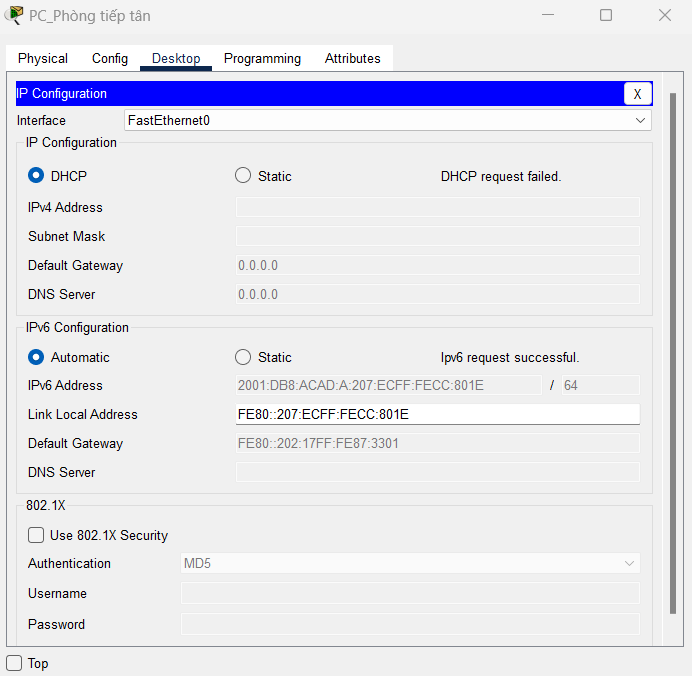
\includegraphics[width=16cm, height=14cm]{img/getDHCP.png}
    \caption{Các PC lấy DHCPv4 và DHCPv6 thành công}
    \label{hinh4131a}
\end{figure}
\cleardoublepage

\section*{CHƯƠNG 5 - KẾT LUẬN}
\addcontentsline{toc}{section}{\numberline{}CHƯƠNG 5 - KẾT LUẬN}
\hspace*{0.25cm}Bộ phận hệ thống đã được thiết kế và cấu hình trên Cisco Packet Tracer. Mô hình đáp ứng được các yêu cầu cơ bản vể địa chỉ đưa ra như các máy có thể ping được với nhau. Ngoài ra, các phòng chức năng cũng được cấu hình mạng không dây với cấu hình bảo mật WPA2- Enterprise\\
\hspace*{1cm}Để mô hình hệ thống mạng được hoàn thiện hơn trong tương lai thì chúng ta cần phải nâng cấp tính bảo mật của mô hình. Thêm một số tính năng cần thiết như mở rộng thêm nhiều điểm truy cập, mở rộng mô hình thêm nhiều thiết bị hơn
\cleardoublepage

\section*{TÀI LIỆU THAM KHẢO}
\addcontentsline{toc}{section}{\numberline{}TÀI LIỆU THAM KHẢO}
\hspace*{0.25cm}[1] 11.7.5 Packet Tracer – Subnetting Scenario.https://itexamanswers.net/11-7-5-packet-tracer-subnetting-scenario-instruction-answers.html\\
\cleardoublepage

\section*{PHỤ LỤC}
\addcontentsline{toc}{section}{\numberline{}PHỤ LỤC}
\hspace*{1cm}[1] \textbf{Password truy cập vào WLC } :\\
\hspace*{2cm} WLC\_TPHCM : https://192.168.200.2, user: admin , password: Cisco123\\
\cleardoublepage
\end{document}
